% !TEX program = pdflatex
\documentclass[13pt,a4paper,twoside]{report}

% ============================================================================
% PACKAGES
% ============================================================================
\usepackage[utf8]{vntex}                % Tiếng Việt
\usepackage{amsmath,amssymb,amsfonts}   % Toán học
\usepackage{graphicx}                   % Hình ảnh
\usepackage{float}                      % [H] cho hình ảnh
\usepackage[top=25mm,bottom=25mm,left=30mm,right=25mm]{geometry}
\usepackage{setspace}                   % Giãn dòng
\usepackage{indentfirst}                % Thụt dòng đầu tiên
\usepackage{titlesec}                   % Tùy chỉnh heading
\usepackage{tocloft}                    % Tùy chỉnh mục lục
\usepackage{hyperref}                   % Siêu liên kết
\usepackage{cite}                       % Trích dẫn
\usepackage{enumitem}                   % Danh sách
\usepackage{tabularx}                   % Bảng
\usepackage{booktabs}                   % Bảng đẹp
\usepackage{longtable}                  % Bảng dài
\usepackage{multirow}                   % Merge row trong bảng
\usepackage{array}                      % Tùy chỉnh cột bảng
\usepackage{caption}                    % Chú thích
\usepackage{fancyhdr}                   % Header/footer
\usepackage[nottoc]{tocbibind}          % TOC với references
\usepackage{makecell}                   % Ô trong bảng
\usepackage{xcolor}                     % Màu sắc
\usepackage{tikz}                       % Vẽ sơ đồ
\usepackage{listings}                   % Code listing
\usepackage{appendix}                   % Phụ lục

% ============================================================================
% LISTINGS CONFIG
% ============================================================================
\lstset{
  basicstyle=\ttfamily\small,
  breaklines=true,
  frame=single,
  numbers=left,
  numberstyle=\tiny,
  showstringspaces=false,
  tabsize=2
}

% ============================================================================
% SPACING
% ============================================================================
\onehalfspacing

% ============================================================================
% HEADER / FOOTER
% ============================================================================
\pagestyle{fancy}
\fancyhf{}
\fancyhead[LE,RO]{\thepage}
\fancyhead[RE]{\leftmark}
\fancyhead[LO]{\rightmark}
\renewcommand{\headrulewidth}{0.4pt}

% ============================================================================
% HYPERREF SETUP
% ============================================================================
\hypersetup{
  colorlinks=true,
  linkcolor=black,
  citecolor=black,
  urlcolor=blue
}

% ============================================================================
% TOC SETTINGS
% ============================================================================
\setcounter{secnumdepth}{3}
\setcounter{tocdepth}{2}

% ============================================================================
% TITLE FORMAT (Heading giống template HUST)
% ============================================================================
\titleformat{\chapter}[display]
  {\normalfont\bfseries\fontsize{16}{20}\selectfont}
  {\centering\MakeUppercase{\chaptername}\ \thechapter}
  {12pt}
  {\centering\fontsize{16}{20}\selectfont}
\titlespacing*{\chapter}{0pt}{0pt}{20pt}

\titleformat{\section}
  {\normalfont\bfseries\fontsize{14}{18}\selectfont}
  {\thesection}
  {6pt}
  {}
\titlespacing*{\section}{0pt}{12pt}{6pt}

\titleformat{\subsection}
  {\normalfont\bfseries\fontsize{13}{16}\selectfont}
  {\thesubsection}
  {6pt}
  {}
\titlespacing*{\subsection}{0pt}{12pt}{6pt}

\titleformat{\subsubsection}
  {\normalfont\bfseries\fontsize{13}{16}\selectfont}
  {\thesubsubsection}
  {6pt}
  {}
\titlespacing*{\subsubsection}{0pt}{12pt}{6pt}

% ============================================================================
% BEGIN DOCUMENT
% ============================================================================
\begin{document}

% ============================================================================
% COVER PAGE (TRANG BÌA)
% ============================================================================
\thispagestyle{empty}
\begin{center}
  \vspace*{1cm}
  {\fontsize{13}{16}\selectfont TRƯỜNG ĐẠI HỌC BÁCH KHOA HÀ NỘI}\\[4pt]
  {\fontsize{13}{16}\selectfont VIỆN CÔNG NGHỆ THÔNG TIN VÀ TRUYỀN THÔNG}\\[4pt]
  \rule{\textwidth}{1pt}\\[4pt]
  {\fontsize{13}{16}\selectfont ──────── * ────────}

  \vspace{3cm}

  {\fontsize{18}{22}\bfseries BÁO CÁO}\\[8pt]
  {\fontsize{14}{18}\bfseries MÔN: Project III}

  \vspace{2cm}

  {\fontsize{16}{20}\bfseries\MakeUppercase{Thiết kế và xây dựng nền tảng đặt phòng}\\}
  {\fontsize{16}{20}\bfseries\MakeUppercase{khách sạn trực tuyến TravelNest}}

  \vspace{2.5cm}

  \begin{tabbing}
    \hspace{4cm}\= \kill
    \textbf{Sinh viên thực hiện:} \> Lê Đức Phương -- 20225380 \\[6pt]
    \textbf{Lớp:} \> Kỹ thuật máy tính 01 -- K67 \\[6pt]
    \textbf{Giảng viên hướng dẫn:} \> TS. Trần Hải Anh
  \end{tabbing}

  \vspace{3cm}

  {\fontsize{13}{16}\selectfont HÀ NỘI, 07/2026}
\end{center}

\newpage

% ============================================================================
% TRANG BÌA PHỤ (SUB-COVER)
% ============================================================================
\thispagestyle{empty}
\begin{center}
  \vspace*{1cm}
  {\fontsize{13}{16}\selectfont TRƯỜNG ĐẠI HỌC BÁCH KHOA HÀ NỘI}\\[4pt]
  {\fontsize{13}{16}\selectfont VIỆN CÔNG NGHỆ THÔNG TIN VÀ TRUYỀN THÔNG}\\[4pt]
  \rule{\textwidth}{1pt}\\[4pt]
  {\fontsize{13}{16}\selectfont ──────── * ────────}

  \vspace{3cm}

  {\fontsize{18}{22}\bfseries BÁO CÁO}\\[8pt]
  {\fontsize{14}{18}\bfseries MÔN: Project III}

  \vspace{2cm}

  {\fontsize{16}{20}\bfseries\MakeUppercase{Thiết kế và xây dựng nền tảng đặt phòng}\\}
  {\fontsize{16}{20}\bfseries\MakeUppercase{khách sạn trực tuyến TravelNest}}

  \vspace{2.5cm}

  \begin{tabbing}
    \hspace{4cm}\= \kill
    \textbf{Sinh viên thực hiện:} \> Lê Đức Phương -- 20225380 \\[6pt]
    \textbf{Lớp:} \> Kỹ thuật máy tính 01 -- K67 \\[6pt]
    \textbf{Giảng viên hướng dẫn:} \> TS. Trần Hải Anh \\[6pt]
    \textbf{Chữ ký GVHD:} \> \hspace{3cm} \\[6pt]
    \textbf{Khoa:} \> Kỹ thuật máy tính \\[6pt]
    \textbf{Trường:} \> Công nghệ Thông tin và Truyền thông
  \end{tabbing}

  \vspace{3cm}

  {\fontsize{13}{16}\selectfont HÀ NỘI, 07/2026}
\end{center}

\newpage
\thispagestyle{empty}
\null
\newpage

% ============================================================================
% LỜI CAM ĐOAN
% ============================================================================
\chapter*{LỜI CAM ĐOAN}
\addcontentsline{toc}{chapter}{LỜI CAM ĐOAN}

Em xin cam đoan đồ án tốt nghiệp với đề tài "Xây dựng hệ thống đặt phòng khách sạn TravelNest" là công trình nghiên cứu và phát triển do em thực hiện, dưới sự hướng dẫn của TS. Trần Hải Anh. Các nội dung trình bày trong báo cáo là trung thực, không sao chép từ bất kỳ công trình nào khác. Những tài liệu, công nghệ và mã nguồn mở tham khảo trong quá trình thực hiện đề tài đều được trích dẫn và ghi rõ nguồn trong phần Tài liệu tham khảo.

Em xin hoàn toàn chịu trách nhiệm về nội dung của báo cáo này.

\vspace{1cm}
\begin{flushright}
  \begin{minipage}{5cm}
    \centering
    \hrule
    \textbf{Lê Đức Phương}
  \end{minipage}
\end{flushright}

\newpage

% ============================================================================
% LỜI CẢM ƠN
% ============================================================================
\chapter*{LỜI CẢM ƠN}
\addcontentsline{toc}{chapter}{LỜI CẢM ƠN}

Lời đầu tiên, em xin gửi lời cảm ơn chân thành và sâu sắc nhất đến TS. Trần Hải Anh, giảng viên hướng dẫn của em trong quá trình thực hiện đề tài này. Thầy đã tận tình chỉ bảo, định hướng và đưa ra những lời khuyên quý báu, giúp em có được những kiến thức và kinh nghiệm thực tiễn trong suốt quá trình nghiên cứu và phát triển sản phẩm.

Em cũng xin gửi lời cảm ơn đến các thầy cô trong Viện Công nghệ Thông tin và Truyền thông, Trường Đại học Bách khoa Hà Nội, những người đã trang bị cho em nền tảng kiến thức vững chắc trong suốt những năm học vừa qua. Những kiến thức về công nghệ phần mềm, cơ sở dữ liệu, mạng máy tính và các môn học chuyên ngành khác là hành trang không thể thiếu để em hoàn thành được dự án này.

Cuối cùng, em xin cảm ơn gia đình, bạn bè và những người thân yêu đã luôn ở bên, động viên và hỗ trợ em trong suốt quá trình học tập và thực hiện dự án.

\vspace{1cm}
\begin{flushright}
  \begin{minipage}{5cm}
    \centering
    \hrule
    \textbf{Lê Đức Phương}
  \end{minipage}
\end{flushright}

\newpage

% ============================================================================
% TÓM TẮT NỘI DUNG BÁO CÁO
% ============================================================================
\chapter*{TÓM TẮT NỘI DUNG BÁO CÁO}
\addcontentsline{toc}{chapter}{TÓM TẮT NỘI DUNG BÁO CÁO}

Trong bối cảnh ngành du lịch trực tuyến đang phát triển bùng nổ trên toàn cầu, các nền tảng đặt phòng khách sạn như Booking.com, Agoda hay Traveloka đã trở thành công cụ quen thuộc của hàng triệu người dùng. Tuy nhiên, các nền tảng này thường được phát triển bởi các tập đoàn lớn với kiến trúc phức tạp, chi phí vận hành cao, và ít có cơ hội để sinh viên hay các nhà phát triển độc lập tiếp cận và học hỏi cách xây dựng một hệ thống hoàn chỉnh từ đầu. Bên cạnh đó, các giải pháp mã nguồn mở hiện có thường thiếu tính toàn diện, không bao gồm đầy đủ các tính năng thực tế như thanh toán trực tuyến, phân tích dữ liệu, xử lý ảnh, hay triển khai trên môi trường production.

Trước thực trạng đó, hướng tiếp cận của đồ án này là xây dựng một hệ thống đặt phòng khách sạn hoàn chỉnh mang tên TravelNest, áp dụng kiến trúc hybrid kết hợp giữa mô hình monolithic cho khối nghiệp vụ lõi và các microservice được viết bằng Go cho các dịch vụ phụ trợ như phân tích dữ liệu (analytics), xử lý ảnh (media), và gửi thông báo (notification). Hệ thống sử dụng NATS JetStream làm bus sự kiện trung tâm để giao tiếp bất đồng bộ giữa các dịch vụ, đồng thời áp dụng mô hình GitOps với Kubernetes và Argo CD để tự động hóa quy trình triển khai.

Giải pháp TravelNest bao gồm hai giao diện người dùng: một ứng dụng web cho khách hàng (Vue 3) để tìm kiếm và đặt phòng, và một bảng điều khiển quản trị (Nuxt 4) cho chủ khách sạn để quản lý danh sách phòng, đơn đặt, và theo dõi doanh thu. Hệ thống backend được xây dựng trên Node.js/Express với Sequelize ORM kết nối MySQL, tích hợp Elasticsearch cho tìm kiếm toàn văn và gợi ý địa điểm, Redis cho caching và hàng đợi công việc, cùng các cơ sở dữ liệu chuyên biệt như MongoDB và ClickHouse cho phân tích dữ liệu.

Kết quả đạt được là hệ thống TravelNest mã nguồn mở với đầy đủ các tính năng cần thiết của một nền tảng đặt phòng thực tế: tìm kiếm theo thời gian thực, đặt phòng với cơ chế giữ chỗ tạm thời, thanh toán qua Stripe, đánh giá và phản hồi, phân tích xu hướng, xử lý ảnh tự động, và thông báo đa kênh. Hệ thống đã được triển khai thành công trên môi trường Kubernetes và có thể truy cập công khai tại \url{https://deployserver.work}.

\vspace{1cm}
\begin{flushright}
  \begin{minipage}{5cm}
    \centering
    \hrule
    \textbf{Sinh viên thực hiện}\\[4pt]
    \textit{(Ký và ghi rõ họ tên)}
  \end{minipage}
\end{flushright}

\newpage

% ============================================================================
% ABSTRACT (English)
% ============================================================================
\chapter*{ABSTRACT}
\addcontentsline{toc}{chapter}{ABSTRACT}

In the context of the rapidly growing online travel industry, hotel booking platforms such as Booking.com, Agoda, and Traveloka have become essential tools for millions of users worldwide. However, these platforms are typically developed by large corporations with complex architectures and high operational costs, offering limited opportunities for students and independent developers to learn how to build a complete system from the ground up. Furthermore, existing open-source solutions often lack comprehensiveness, missing critical real-world features such as online payments, data analytics, image processing, and production-grade deployment.

To address this gap, this project adopts an approach of building a complete hotel booking system named TravelNest, employing a hybrid architecture that combines a monolithic core for business logic with Go-based microservices for auxiliary functions including analytics, media processing, and notifications. The system leverages NATS JetStream as a central event bus for asynchronous inter-service communication and adopts GitOps practices with Kubernetes and Argo CD for automated deployment.

The TravelNest solution consists of two user interfaces: a Vue 3 web application for guests to search and book hotels, and a Nuxt 4 admin dashboard for property owners to manage listings, bookings, and track revenue. The backend is built on Node.js/Express with Sequelize ORM connecting to MySQL, integrating Elasticsearch for full-text search and location suggestions, Redis for caching and job queues, along with specialized databases such as MongoDB and ClickHouse for data analytics.

As a result, TravelNest delivers an open-source, feature-complete hotel booking system with real-time search, temporary hold-based reservations, Stripe payment integration, review and feedback management, trend analytics, automated image processing, and multi-channel notifications. The system has been successfully deployed on a Kubernetes environment and is publicly accessible at \url{https://deployserver.work}.

\newpage

% ============================================================================
% TABLE OF CONTENTS
% ============================================================================
\renewcommand{\contentsname}{MỤC LỤC}
\tableofcontents
\newpage

% ============================================================================
% LIST OF FIGURES
% ============================================================================
\renewcommand{\listfigurename}{DANH MỤC HÌNH VẼ}
\listoffigures
\newpage

% ============================================================================
% LIST OF TABLES
% ============================================================================
\renewcommand{\listtablename}{DANH MỤC BẢNG BIỂU}
\listoftables
\newpage

% ============================================================================
% DANH MỤC THUẬT NGỮ VÀ TỪ VIẾT TẮT
% ============================================================================
\chapter*{DANH MỤC THUẬT NGỮ VÀ TỪ VIẾT TẮT}
\addcontentsline{toc}{chapter}{DANH MỤC THUẬT NGỮ VÀ TỪ VIẾT TẮT}

\begin{longtable}{p{4cm} p{11cm}}
  \textbf{Thuật ngữ} & \textbf{Ý nghĩa} \\
  \hline
  API & Giao diện lập trình ứng dụng (Application Programming Interface) \\
  BullMQ & Thư viện hàng đợi công việc dựa trên Redis cho Node.js \\
  CI/CD & Tích hợp liên tục / Triển khai liên tục (Continuous Integration / Continuous Deployment) \\
  CSS & Ngôn ngữ định kiểu (Cascading Style Sheets) \\
  ERD & Biểu đồ thực thể - liên kết (Entity-Relationship Diagram) \\
  GitOps & Phương pháp triển khai dựa trên Git làm nguồn sự thật duy nhất \\
  HTML & Ngôn ngữ đánh dấu siêu văn bản (HyperText Markup Language) \\
  IDE & Môi trường phát triển tích hợp (Integrated Development Environment) \\
  JSON & Định dạng trao đổi dữ liệu (JavaScript Object Notation) \\
  K8s & Kubernetes -- Hệ thống điều phối container \\
  MVC & Mô hình - Khung nhìn - Điều khiển (Model-View-Controller) \\
  NATS & Hệ thống nhắn tin phân tán hiệu năng cao (Neural Autonomic Transport System) \\
  NoSQL & Cơ sở dữ liệu phi quan hệ (Not Only SQL) \\
  ORM & Ánh xạ đối tượng - quan hệ (Object-Relational Mapping) \\
  REST & Kiến trúc truyền tải trạng thái biểu diễn (Representational State Transfer) \\
  SPA & Ứng dụng web đơn trang (Single Page Application) \\
  SQL & Ngôn ngữ truy vấn có cấu trúc (Structured Query Language) \\
  SSR & Server-Side Rendering -- Kết xuất giao diện phía máy chủ \\
  UML & Ngôn ngữ mô hình hóa thống nhất (Unified Modeling Language) \\
\end{longtable}

\newpage

% ============================================================================
% CHƯƠNG 1: GIỚI THIỆU ĐỀ TÀI
% ============================================================================
\chapter{GIỚI THIỆU ĐỀ TÀI}

Ngành du lịch toàn cầu đã chứng kiến sự chuyển đổi mạnh mẽ trong hai thập kỷ qua, với sự bùng nổ của các nền tảng đặt phòng trực tuyến. Theo báo cáo của Statista, doanh thu thị trường đặt phòng khách sạn trực tuyến toàn cầu dự kiến đạt hơn 700 tỷ USD vào năm 2025 \cite{booking2025statista}. Tại Việt Nam, xu hướng này cũng không ngoại lệ khi ngày càng nhiều người dùng chuyển từ hình thức đặt phòng truyền thống sang các nền tảng trực tuyến để tìm kiếm, so sánh giá cả và đặt phòng một cách nhanh chóng.

Bên cạnh nhu cầu của khách du lịch, các chủ khách sạn và cơ sở lưu trú cũng đang đối mặt với bài toán quản lý hiệu quả: từ quản lý danh sách phòng, giá cả theo mùa, tình trạng phòng trống theo thời gian thực, đến theo dõi doanh thu và tương tác với khách hàng. Một hệ thống quản lý toàn diện có thể giúp các chủ khách sạn tối ưu hóa hoạt động kinh doanh và nâng cao trải nghiệm khách hàng.

\section{Đặt vấn đề}

Trên thị trường hiện nay, các nền tảng đặt phòng khách sạn lớn như Booking.com, Agoda, Expedia và Traveloka đã xây dựng được vị thế vững chắc với hàng triệu người dùng trên toàn cầu. Các nền tảng này sở hữu lượng dữ liệu khổng lồ, thuật toán tìm kiếm và gợi ý tinh vi, cùng hệ thống thanh toán và chăm sóc khách hàng chuyên nghiệp. Tuy nhiên, các hệ thống này được phát triển và vận hành bởi các tập đoàn công nghệ lớn với đội ngũ kỹ sư đông đảo, ngân sách khổng lồ, và kiến trúc hệ thống cực kỳ phức tạp. Đối với sinh viên công nghệ thông tin, việc tiếp cận mã nguồn và kiến trúc bên trong của các hệ thống này là điều không thể, gây khó khăn cho việc học tập và nghiên cứu về cách xây dựng một hệ thống thương mại điện tử hoàn chỉnh trong thực tế.

Bên cạnh đó, các giải pháp mã nguồn mở hiện có cho lĩnh vực đặt phòng khách sạn thường có phạm vi hạn chế. Chúng thường chỉ tập trung vào một khía cạnh cụ thể như giao diện tìm kiếm đơn giản hoặc quản lý đặt phòng cơ bản, thiếu đi các tính năng quan trọng trong thực tế như: tìm kiếm toàn văn với Elasticsearch, thanh toán trực tuyến qua cổng thanh toán thực tế (Stripe), phân tích dữ liệu và xu hướng, xử lý ảnh tự động, gửi thông báo đa kênh (email, SMS, thời gian thực), hay khả năng triển khai trên môi trường production với Kubernetes. Ngoài ra, hầu hết các dự án mã nguồn mở không áp dụng kiến trúc microservice hoặc các mô hình kiến trúc hiện đại, khiến người học khó có cơ hội tiếp cận với các xu hướng phát triển phần mềm mới nhất.

Từ những hạn chế trên, có thể thấy rằng việc xây dựng một hệ thống đặt phòng khách sạn mã nguồn mở, hoàn chỉnh về mặt tính năng, hiện đại về mặt kiến trúc, và có khả năng triển khai thực tế là một nhu cầu cấp thiết cho cả mục đích học tập lẫn ứng dụng thực tiễn. Nếu được giải quyết, hệ thống này không chỉ là một công cụ học tập quý giá cho sinh viên và các nhà phát triển phần mềm, mà còn có thể được sử dụng như một nền tảng khởi đầu cho các doanh nghiệp vừa và nhỏ trong lĩnh vực du lịch và khách sạn.

\section{Mục tiêu và phạm vi đề tài}

Trên cơ sở phân tích thực trạng và các hạn chế của các hệ thống hiện có, đề tài này hướng tới mục tiêu xây dựng một nền tảng đặt phòng khách sạn trực tuyến hoàn chỉnh mang tên TravelNest, với các mục tiêu cụ thể như sau:

\begin{enumerate}
  \item \textbf{Đối với khách du lịch:} Xây dựng một ứng dụng web cho phép người dùng tìm kiếm khách sạn theo nhiều tiêu chí (vị trí địa lý, ngày nhận/phòng, mức giá, tiện nghi, đánh giá), xem thông tin chi tiết về phòng và giá cả theo thời gian thực, thực hiện đặt phòng với cơ chế giữ chỗ tạm thời, thanh toán trực tuyến qua Stripe, quản lý đơn đặt, và viết đánh giá sau khi lưu trú.
  \item \textbf{Đối với chủ khách sạn:} Phát triển một bảng điều khiển quản trị cho phép chủ khách sạn quản lý danh sách khách sạn, phòng, giá cả, tình trạng phòng trống, chính sách hủy phòng, xem và quản lý đơn đặt phòng, phản hồi đánh giá của khách hàng, theo dõi doanh thu và các chỉ số phân tích.
  \item \textbf{Về mặt kiến trúc:} Áp dụng kiến trúc hybrid kết hợp monolithic (Node.js/Express) cho khối nghiệp vụ lõi và các microservice (Go) cho các dịch vụ phụ trợ, sử dụng NATS JetStream làm bus sự kiện và triển khai trên Kubernetes với GitOps thông qua Argo CD.
\end{enumerate}

Phạm vi của đề tài tập trung vào việc xây dựng một hệ thống hoàn chỉnh có thể hoạt động trong môi trường thực tế, với đầy đủ các chức năng từ tìm kiếm, đặt phòng, thanh toán, đến phân tích dữ liệu và thông báo. Tuy nhiên, đề tài không bao gồm các khía cạnh như ứng dụng di động native, hệ thống khuyến nghị dựa trên trí tuệ nhân tạo, hay tích hợp với các kênh phân phối bên thứ ba (channel manager). Các tính năng này được đề xuất như hướng phát triển trong tương lai.

\section{Định hướng giải pháp}

Để giải quyết các vấn đề đã nêu, đề tài lựa chọn định hướng xây dựng một hệ thống web full-stack theo kiến trúc hybrid microservice. Hướng tiếp cận này được lựa chọn vì các lý do sau:

Thứ nhất, kiến trúc monolithic cho khối nghiệp vụ lõi (đặt phòng, thanh toán, quản lý khách sạn) giúp đơn giản hóa việc phát triển ban đầu, đảm bảo tính nhất quán của dữ liệu giao dịch thông qua các transaction ACID của MySQL. Điều này đặc biệt quan trọng đối với các nghiệp vụ nhạy cảm như đặt phòng và thanh toán, nơi mà tính toàn vẹn dữ liệu là yêu cầu bắt buộc.

Thứ hai, việc tách các dịch vụ phụ trợ (phân tích, xử lý ảnh, thông báo) thành các microservice viết bằng Go cho phép tận dụng hiệu năng cao của Go trong các tác vụ xử lý nặng, đồng thời giảm tải cho khối monolithic. Giao tiếp giữa các dịch vụ thông qua NATS JetStream đảm bảo tính bất đồng bộ, khả năng phục hồi và mở rộng của hệ thống.

Thứ ba, việc sử dụng đa dạng các cơ sở dữ liệu chuyên biệt --- MySQL cho dữ liệu giao dịch, Elasticsearch cho tìm kiếm toàn văn, Redis cho caching và hàng đợi, MongoDB và ClickHouse cho phân tích --- cho phép mỗi loại dữ liệu được lưu trữ và truy vấn theo cách tối ưu nhất, thay vì cố gắng dùng một cơ sở dữ liệu duy nhất cho mọi nhu cầu.

Thứ tư, việc triển khai trên Kubernetes với GitOps thông qua Argo CD đảm bảo hệ thống có thể được triển khai một cách nhất quán, tự động và có khả năng mở rộng linh hoạt, đáp ứng các yêu cầu của môi trường production thực tế.

Đóng góp chính của đề tài là một hệ thống đặt phòng khách sạn mã nguồn mở, hoàn chỉnh và sẵn sàng cho production, có thể được sử dụng làm tài liệu tham khảo học thuật hoặc nền tảng khởi đầu cho các dự án thương mại. Hệ thống đã được triển khai thành công và có thể truy cập công khai tại địa chỉ \url{https://deployserver.work}.

\section{Bố cục báo cáo}

Phần còn lại của báo cáo được tổ chức như sau.

Trong Chương 2, em trình bày quá trình khảo sát hiện trạng các hệ thống đặt phòng khách sạn hiện có, từ đó phân tích và đặc tả yêu cầu chức năng và phi chức năng cho hệ thống TravelNest. Các biểu đồ use case tổng quát và phân rã được sử dụng để mô hình hóa các tác nhân và chức năng của hệ thống.

Trong Chương 3, em trình bày các nền tảng lý thuyết và công nghệ được sử dụng trong quá trình phát triển hệ thống. Với mỗi công nghệ, em phân tích lý do lựa chọn và so sánh với các giải pháp thay thế. Các công nghệ bao gồm: nền tảng frontend (Vue 3, Nuxt 4), backend (Node.js/Express, Go), cơ sở dữ liệu (MySQL, Redis, Elasticsearch, MongoDB), cơ chế giao tiếp bất đồng bộ (NATS JetStream), và các công cụ triển khai (Docker, Kubernetes, Argo CD).

Trong Chương 4, em tập trung vào quá trình phân tích thiết kế và triển khai hệ thống. Chương này bao gồm các nội dung: lựa chọn kiến trúc phần mềm, thiết kế tổng quan với biểu đồ gói UML, thiết kế chi tiết các module, thiết kế cơ sở dữ liệu với 47 bảng, xây dựng ứng dụng với 15 nhóm API, kiểm thử, và triển khai hệ thống trên Kubernetes với Argo CD.

Trong Chương 5, em trình bày các giải pháp và đóng góp nổi bật của đề tài, bao gồm: chiến lược di chuyển từ monolithic sang microservice theo mô hình Strangler Fig, kiến trúc giao tiếp bất đồng bộ với NATS JetStream, hệ thống tìm kiếm khách sạn với Elasticsearch, và cơ chế thanh toán an toàn với sổ cái kép (double-entry ledger).

Trong Chương 6, em tổng kết các kết quả đạt được, so sánh với các hệ thống tương tự, rút ra bài học kinh nghiệm, và đề xuất các hướng phát triển trong tương lai cho hệ thống TravelNest.

% ============================================================================
% CHƯƠNG 2: KHẢO SÁT VÀ PHÂN TÍCH YÊU CẦU
% ============================================================================
\chapter{KHẢO SÁT VÀ PHÂN TÍCH YÊU CẦU}

Chương 1 đã giới thiệu tổng quan về đề tài, đặt vấn đề và định hướng giải pháp cho hệ thống TravelNest. Trong chương này, em đi sâu vào quá trình khảo sát hiện trạng các hệ thống đặt phòng khách sạn hiện có trên thị trường, phân tích yêu cầu chức năng và phi chức năng của hệ thống, từ đó làm cơ sở cho quá trình thiết kế và phát triển trong các chương tiếp theo.

\section{Khảo sát hiện trạng}

Để xây dựng một hệ thống đặt phòng khách sạn có tính cạnh tranh và đáp ứng nhu cầu thực tế của người dùng, việc khảo sát và phân tích các hệ thống hiện có trên thị trường là bước không thể thiếu. Phần này sẽ phân tích ba khía cạnh chính: các nền tảng thương mại hàng đầu, các giải pháp mã nguồn mở hiện có, và nhu cầu của người dùng.

\subsection{Các nền tảng đặt phòng thương mại}

Ba nền tảng đặt phòng khách sạn trực tuyến lớn nhất hiện nay là Booking.com, Agoda và Traveloka. Bảng \ref{tab:competitors} dưới đây tóm tắt so sánh các tính năng chính của ba nền tảng này.

\begin{table}[H]
\centering
\caption{So sánh các nền tảng đặt phòng khách sạn hàng đầu}
\label{tab:competitors}
\begin{tabularx}{\textwidth}{p{2.8cm} X X X}
\toprule
\textbf{Tính năng} & \textbf{Booking.com} & \textbf{Agoda} & \textbf{Traveloka} \\
\midrule
Tìm kiếm theo vị trí & Có & Có & Có \\
Tìm kiếm theo ngày & Có & Có & Có \\
Lọc theo giá, đánh giá & Có & Có & Có \\
Bản đồ tương tác & Có & Có & Có \\
Đa ngôn ngữ & 43+ ngôn ngữ & 38+ ngôn ngữ & 6+ ngôn ngữ \\
Thanh toán trực tuyến & Có & Có & Có \\
Đánh giá và phản hồi & Có & Có & Có \\
Quản lý khách sạn & Có (Extranet) & Có (YCS) & Có \\
Phân tích doanh thu & Có & Có & Hạn chế \\
Ứng dụng di động & Có & Có & Có \\
API mở & Không & Có (hạn chế) & Không \\
\bottomrule
\end{tabularx}
\end{table}

Qua phân tích, có thể nhận thấy các điểm mạnh và hạn chế sau của các nền tảng thương mại:

\textbf{Điểm mạnh:}
\begin{itemize}
  \item Lượng dữ liệu khổng lồ về khách sạn và người dùng, cho phép xây dựng các thuật toán gợi ý và cá nhân hóa mạnh mẽ.
  \item Hệ thống tìm kiếm nhanh và chính xác với khả năng xử lý truy vấn phức tạp, hỗ trợ đa ngôn ngữ.
  \item Tích hợp thanh toán đa dạng, hỗ trợ nhiều loại tiền tệ và phương thức thanh toán toàn cầu.
  \item Đội ngũ phát triển và vận hành chuyên nghiệp, đảm bảo hệ thống hoạt động ổn định 24/7.
\end{itemize}

\textbf{Hạn chế:}
\begin{itemize}
  \item Mã nguồn đóng, không cho phép người học và nhà phát triển độc lập nghiên cứu và tùy chỉnh.
  \item Chi phí hoa hồng cao cho chủ khách sạn (thường từ 15\% đến 25\%).
  \item Kiến trúc phức tạp, không phù hợp để học tập hoặc làm nền tảng cho các dự án vừa và nhỏ.
\end{itemize}

\subsection{Các giải pháp mã nguồn mở}

Bên cạnh các nền tảng thương mại, một số giải pháp mã nguồn mở cho lĩnh vực đặt phòng khách sạn cũng đã được phát triển. Tuy nhiên, qua khảo sát, hầu hết các giải pháp này có những hạn chế đáng kể:

\begin{itemize}
  \item \textbf{Phạm vi hạn chế:} Hầu hết chỉ tập trung vào một khía cạnh duy nhất như website giới thiệu khách sạn hoặc form đặt phòng đơn giản, thiếu các tính năng thực tế như tìm kiếm nâng cao, thanh toán trực tuyến, hay phân tích dữ liệu.
  \item \textbf{Kiến trúc đơn giản:} Đa số sử dụng kiến trúc monolithic thuần túy với LAMP stack (Linux, Apache, MySQL, PHP), không áp dụng các mô hình kiến trúc hiện đại như microservice hay event-driven.
  \item \textbf{Thiếu khả năng mở rộng:} Không có cơ chế caching, tìm kiếm toàn văn, hay xử lý bất đồng bộ, khiến hệ thống khó đáp ứng khi lượng truy cập tăng cao.
  \item \textbf{Thiếu tài liệu và hướng dẫn:} Nhiều dự án không có tài liệu đầy đủ hoặc đã ngừng phát triển từ lâu.
\end{itemize}

Chính vì những hạn chế này, việc xây dựng TravelNest --- một hệ thống mã nguồn mở hoàn chỉnh với kiến trúc hiện đại --- là cần thiết và có giá trị cho cộng đồng phát triển phần mềm.

\subsection{Nhu cầu người dùng}

Hệ thống TravelNest hướng đến hai nhóm người dùng chính với các nhu cầu khác nhau:

\textbf{Nhóm khách du lịch (Guests):}
\begin{itemize}
  \item Tìm kiếm khách sạn nhanh chóng theo vị trí, ngày nhận phòng và trả phòng.
  \item Xem thông tin chi tiết về khách sạn: hình ảnh, tiện nghi, chính sách, đánh giá từ người dùng khác.
  \item So sánh giá phòng theo thời gian thực.
  \item Đặt phòng an toàn với cơ chế giữ chỗ tạm thời và thanh toán trực tuyến.
  \item Quản lý đơn đặt phòng: xem lịch sử, hủy đặt, yêu cầu hoàn tiền.
  \item Viết đánh giá và tải ảnh lên sau khi lưu trú.
  \item Nhận thông báo qua email về tình trạng đặt phòng.
\end{itemize}

\textbf{Nhóm chủ khách sạn (Property Owners/Admins):}
\begin{itemize}
  \item Quản lý danh sách khách sạn: thêm, sửa, xóa thông tin khách sạn và phòng.
  \item Quản lý giá phòng theo mùa, tình trạng phòng trống.
  \item Quản lý đơn đặt phòng: xác nhận, từ chối, theo dõi trạng thái.
  \item Phản hồi đánh giá của khách hàng.
  \item Theo dõi doanh thu và các chỉ số phân tích (số lượt đặt, tỷ lệ hủy, đánh giá trung bình).
  \item Nhận thông báo về đơn đặt mới, đánh giá mới.
\end{itemize}

\section{Tổng quan chức năng}

Dựa trên kết quả khảo sát hiện trạng và nhu cầu người dùng, phần này trình bày tổng quan các chức năng của hệ thống TravelNest thông qua các biểu đồ use case và mô tả quy trình nghiệp vụ chính.

\subsection{Biểu đồ use case tổng quát}

Hệ thống TravelNest có ba tác nhân chính:

\begin{itemize}
  \item \textbf{Khách (Guest):} Người dùng chưa đăng nhập hoặc đã đăng nhập, có thể tìm kiếm khách sạn, xem thông tin, và thực hiện đặt phòng.
  \item \textbf{Người dùng đã xác thực (Authenticated User):} Khách đã đăng nhập, có thêm quyền quản lý đơn đặt, viết đánh giá, và quản lý thông tin cá nhân.
  \item \textbf{Quản trị viên khách sạn (Hotel Admin):} Chủ khách sạn hoặc nhân viên quản lý, có quyền quản lý khách sạn, phòng, đơn đặt, đánh giá, và theo dõi doanh thu.
  \item \textbf{Quản trị viên hệ thống (System Admin):} Người quản lý toàn bộ hệ thống, có quyền quản lý người dùng, phân quyền, và cấu hình hệ thống.
\end{itemize}

\begin{figure}[H]
  \centering
  % PLACEHOLDER: Biểu đồ use case tổng quát
  % \includegraphics[width=0.95\textwidth]{images/use_case_overview.png}
  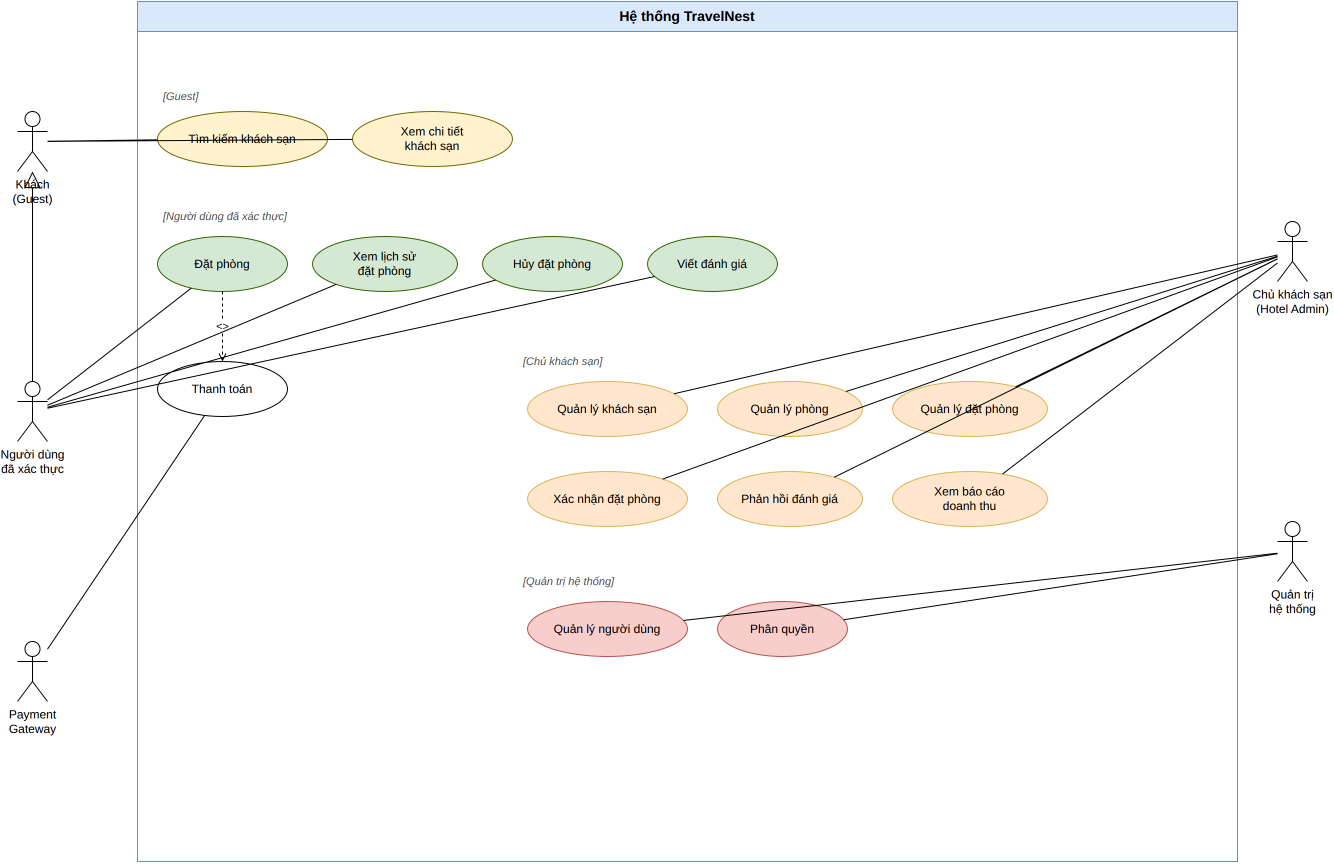
\includegraphics[width=0.95\textwidth]{images/fig_2_1_use_case_overview.png}
  \caption{Biểu đồ use case tổng quát của hệ thống TravelNest}
  \label{fig:use_case_overview}
\end{figure}

Hình \ref{fig:use_case_overview} mô tả biểu đồ use case tổng quát của hệ thống. Các use case chính bao gồm: Tìm kiếm khách sạn, Xem chi tiết khách sạn, Đặt phòng, Thanh toán, Quản lý đơn đặt, Viết đánh giá, Quản lý khách sạn, Quản lý phòng, Quản lý đơn đặt (Admin), Phản hồi đánh giá, và Xem báo cáo doanh thu.

\subsection{Biểu đồ use case phân rã}

\subsubsection{Phân rã use case "Đặt phòng"}

Use case "Đặt phòng" là một trong những chức năng phức tạp nhất của hệ thống, bao gồm nhiều bước từ chọn phòng đến hoàn tất thanh toán. Hình \ref{fig:use_case_booking} mô tả biểu đồ use case phân rã cho chức năng này.

\begin{figure}[H]
  \centering
  % PLACEHOLDER: Biểu đồ use case phân rã Đặt phòng
  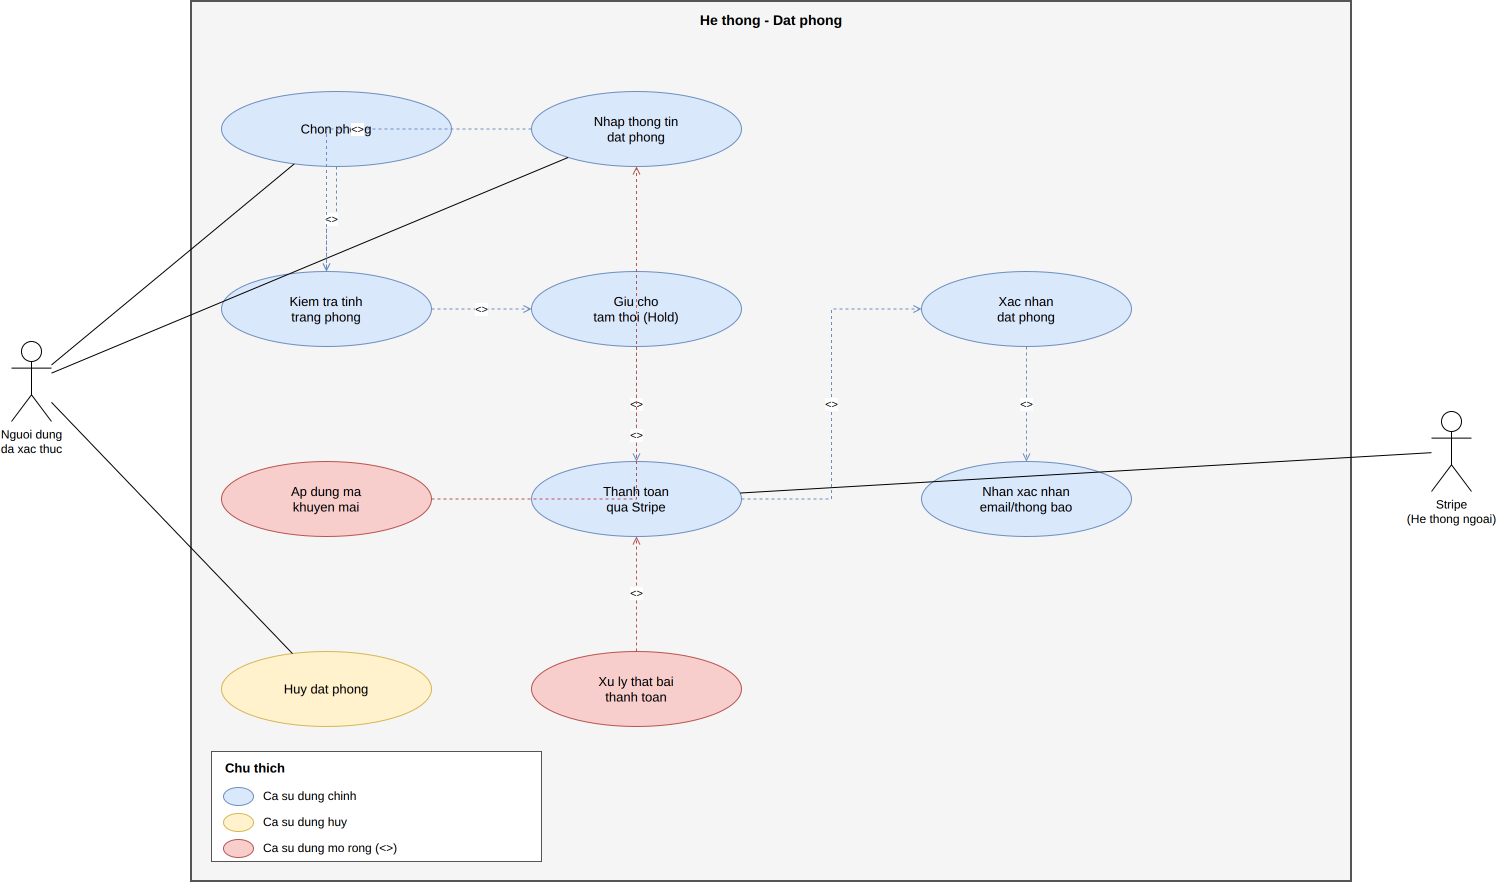
\includegraphics[width=0.95\textwidth]{images/fig_2_2_use_case_booking.png}
  \caption{Biểu đồ use case phân rã chức năng Đặt phòng}
  \label{fig:use_case_booking}
\end{figure}

Use case "Đặt phòng" được phân rã thành các use case con: Chọn phòng, Kiểm tra tình trạng phòng, Giữ chỗ tạm thời (Hold), Thanh toán qua Stripe, và Xác nhận đặt phòng. Use case "Giữ chỗ tạm thời" có quan hệ \texttt{<<include>>} với "Kiểm tra tình trạng phòng" để đảm bảo phòng vẫn còn trống trước khi giữ chỗ.

\subsubsection{Phân rã use case "Quản lý khách sạn"}

\begin{figure}[H]
  \centering
  % PLACEHOLDER: Biểu đồ use case phân rã Quản lý khách sạn
  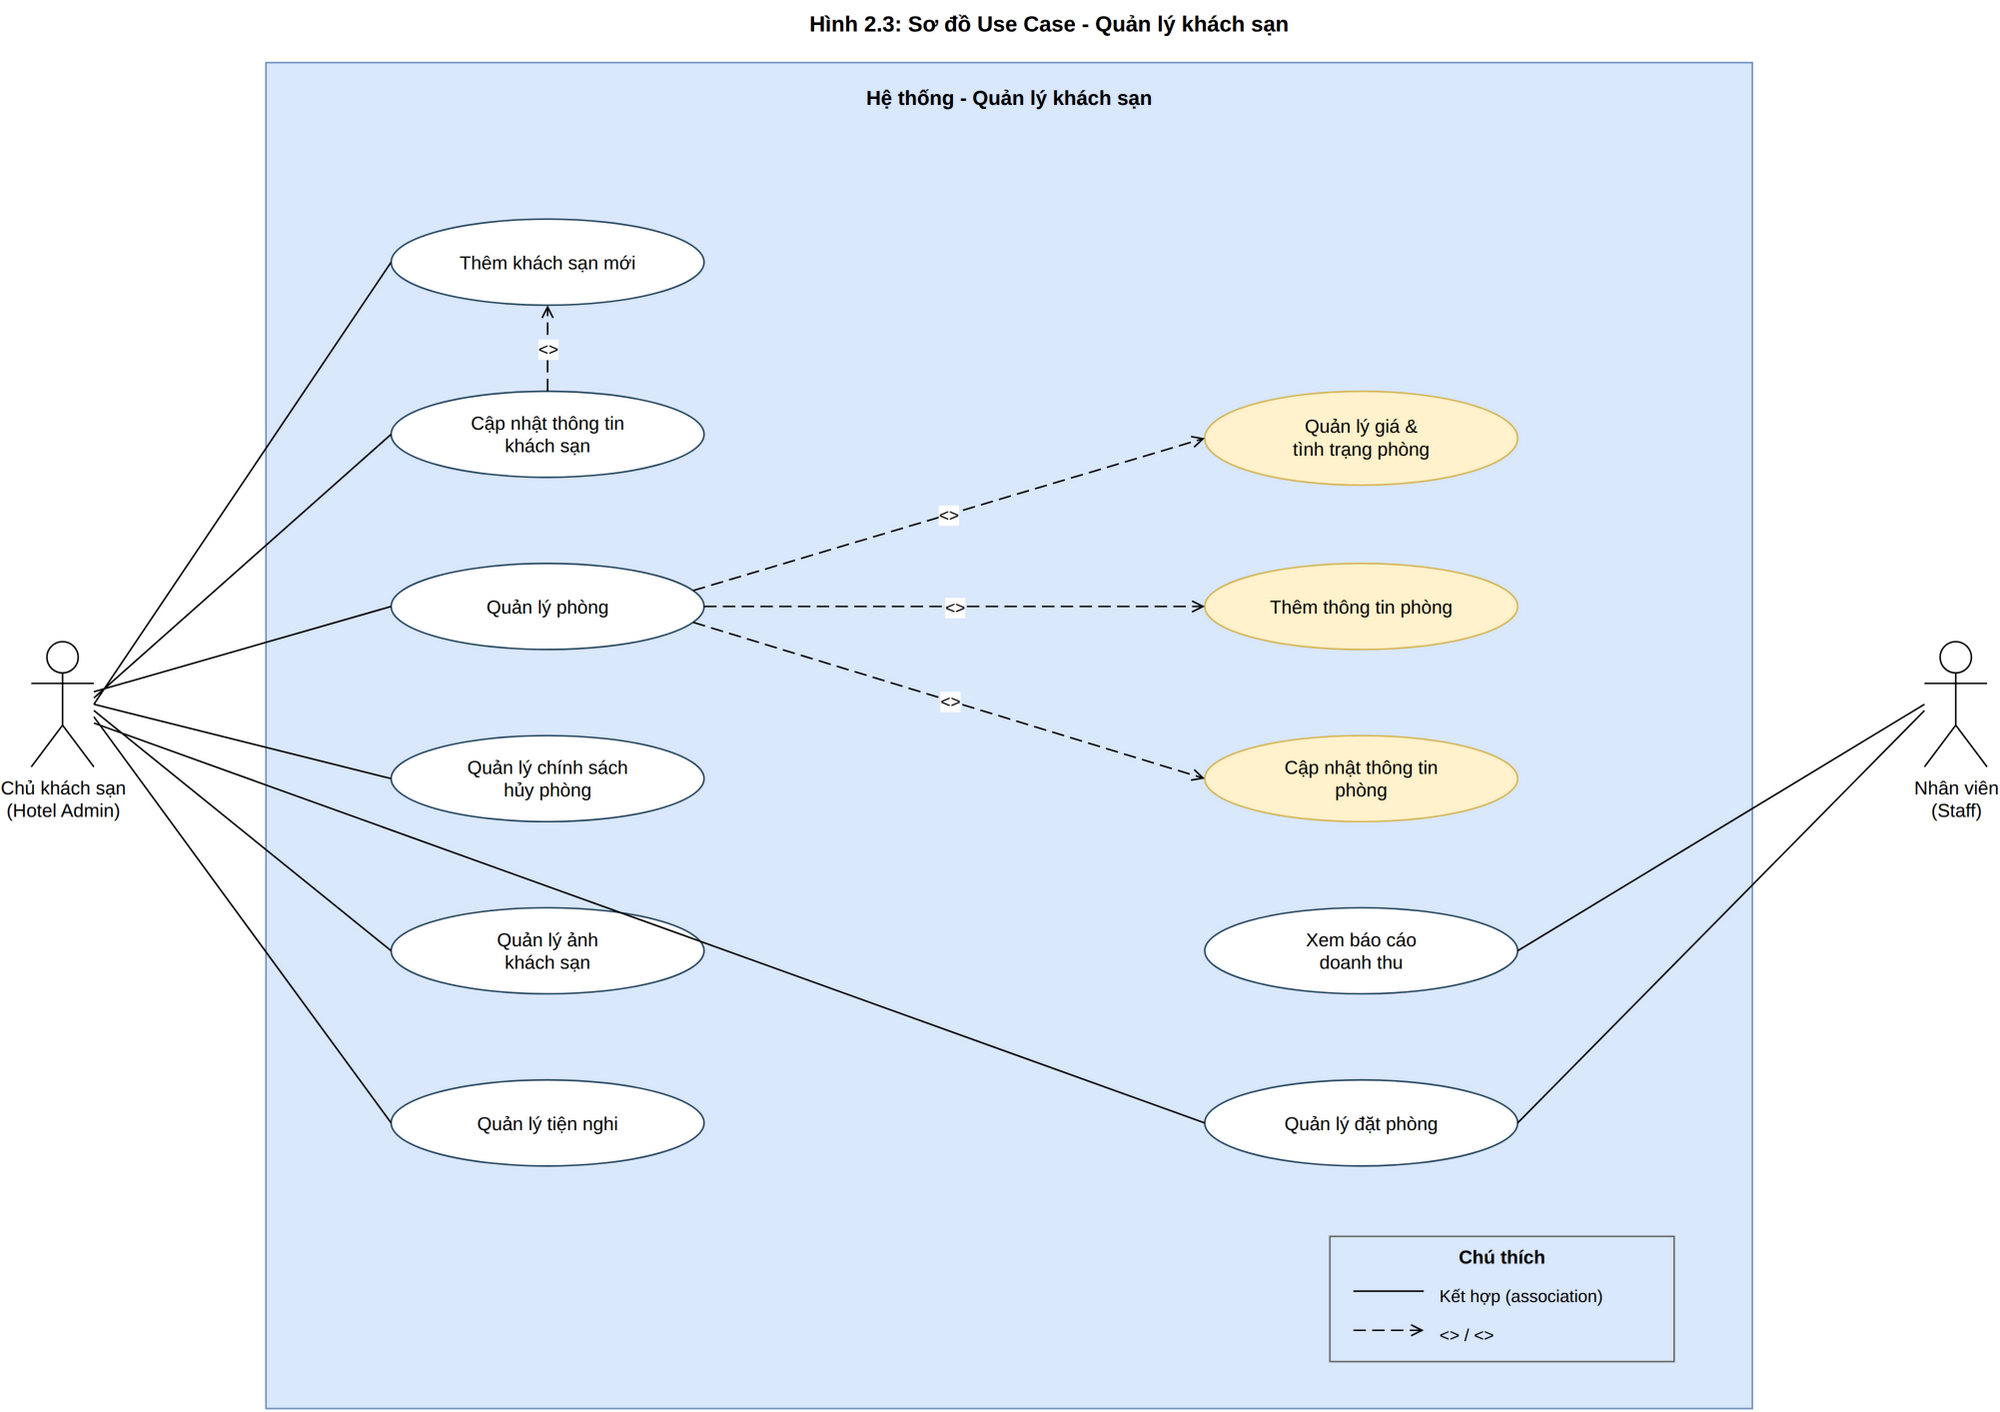
\includegraphics[width=0.95\textwidth]{images/fig_2_3_use_case_hotel_mgmt.png}
  \caption{Biểu đồ use case phân rã chức năng Quản lý khách sạn}
  \label{fig:use_case_hotel_mgmt}
\end{figure}

Hình \ref{fig:use_case_hotel_mgmt} mô tả biểu đồ use case phân rã cho chức năng quản lý khách sạn dành cho chủ khách sạn. Các use case con bao gồm: Thêm khách sạn mới, Cập nhật thông tin khách sạn, Quản lý phòng, Quản lý giá và tình trạng phòng, Quản lý chính sách hủy phòng, Quản lý ảnh khách sạn, và Quản lý tiện nghi.

\subsection{Quy trình nghiệp vụ}

\subsubsection{Quy trình đặt phòng và thanh toán}

Quy trình đặt phòng là quy trình nghiệp vụ cốt lõi của hệ thống TravelNest, kết hợp nhiều use case để hoàn thành một giao dịch đặt phòng. Hình \ref{fig:activity_booking} mô tả biểu đồ hoạt động cho quy trình này.

\begin{figure}[H]
  \centering
  % PLACEHOLDER: Biểu đồ hoạt động quy trình đặt phòng
  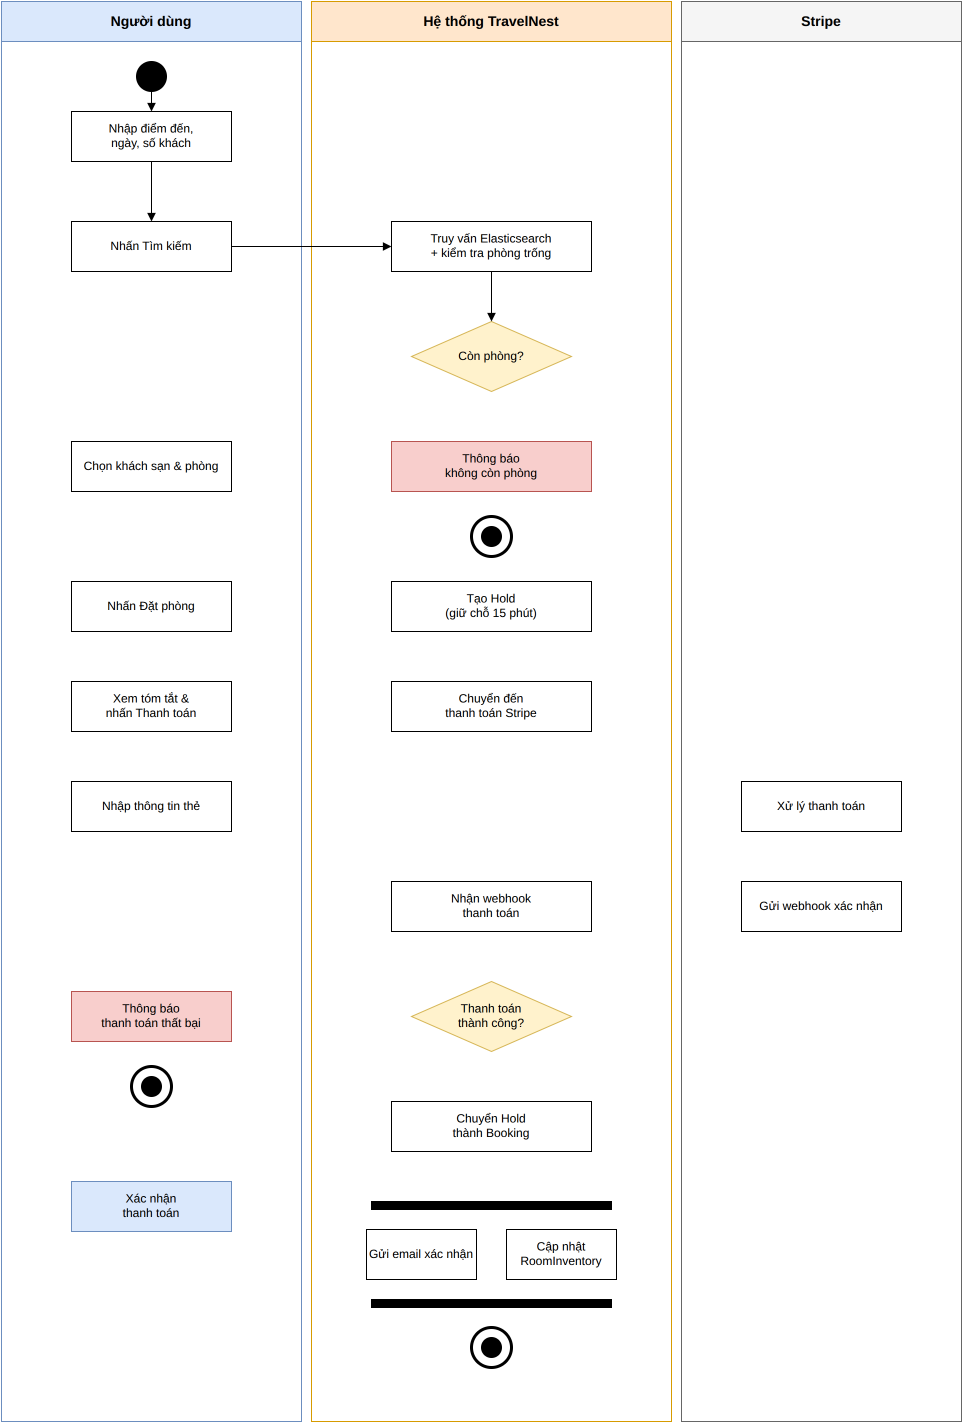
\includegraphics[width=0.95\textwidth]{images/fig_2_4_activity_booking.png}
  \caption{Biểu đồ hoạt động quy trình đặt phòng và thanh toán}
  \label{fig:activity_booking}
\end{figure}

Quy trình đặt phòng tại TravelNest diễn ra theo các bước sau:

\begin{enumerate}
  \item \textbf{Tìm kiếm và chọn phòng:} Người dùng tìm kiếm khách sạn theo vị trí và ngày, chọn phòng phù hợp từ danh sách kết quả.
  \item \textbf{Giữ chỗ tạm thời (Hold):} Hệ thống tạo một bản ghi giữ chỗ (Hold) với thời hạn 15 phút, trong thời gian này phòng được đánh dấu là không khả dụng cho các khách khác.
  \item \textbf{Thanh toán:} Người dùng tiến hành thanh toán qua Stripe. Hệ thống tạo Payment Intent trên Stripe và chờ xác nhận từ phía ngân hàng.
  \item \textbf{Xác nhận đặt phòng:} Khi thanh toán thành công, hệ thống chuyển đổi bản ghi Hold thành Booking chính thức, cập nhật tình trạng phòng, và gửi email xác nhận cho người dùng.
  \item \textbf{Hủy/Hoàn tiền (nếu có):} Nếu người dùng hủy trong thời hạn cho phép, hệ thống xử lý hoàn tiền qua Stripe và cập nhật sổ cái kế toán.
\end{enumerate}

\subsubsection{Quy trình quản lý khách sạn}

\begin{figure}[H]
  \centering
  % PLACEHOLDER: Biểu đồ hoạt động quy trình quản lý khách sạn
  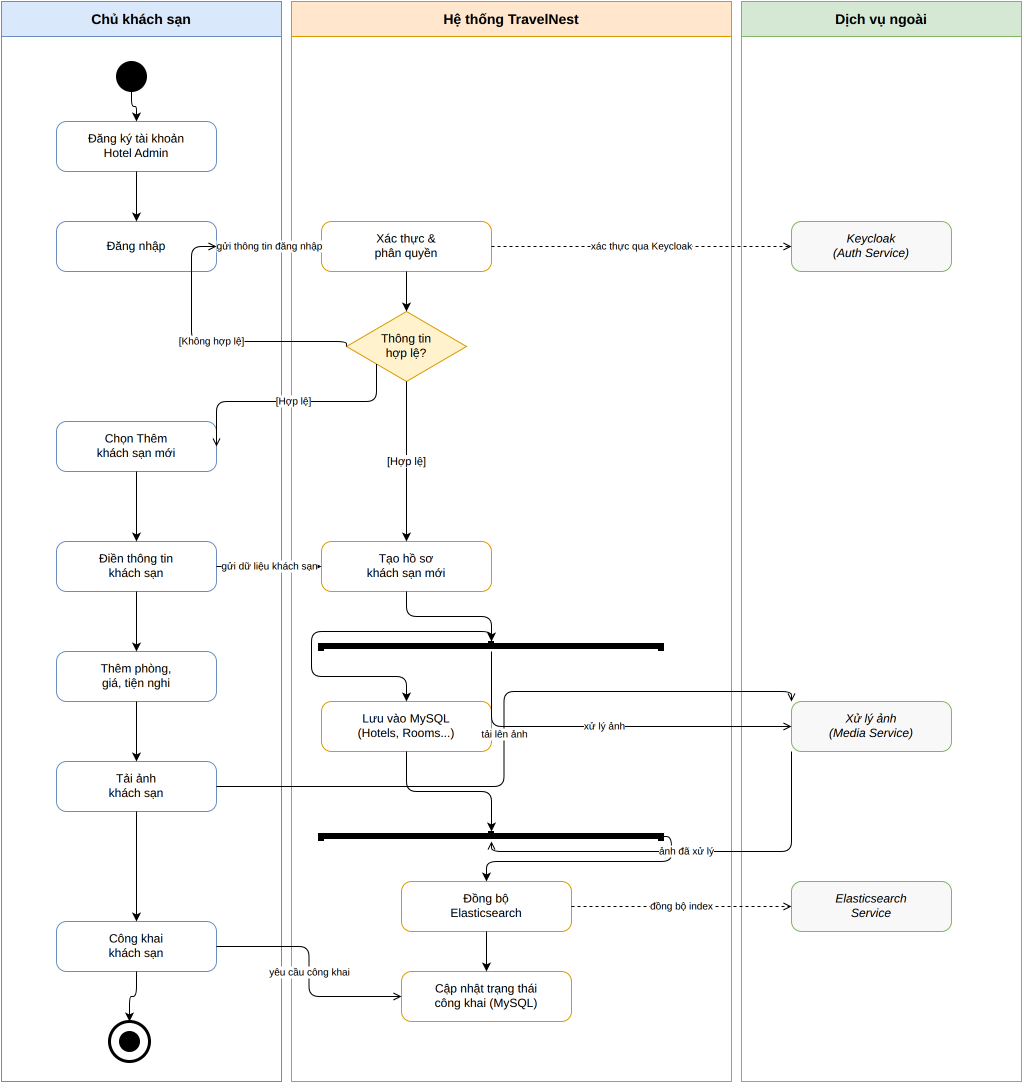
\includegraphics[width=0.95\textwidth]{images/fig_2_5_activity_hotel_mgmt.png}
  \caption{Biểu đồ hoạt động quy trình quản lý khách sạn}
  \label{fig:activity_hotel_mgmt}
\end{figure}

Hình \ref{fig:activity_hotel_mgmt} mô tả quy trình quản lý khách sạn dành cho chủ khách sạn, bao gồm các bước: đăng ký tài khoản chủ khách sạn, tạo hồ sơ khách sạn mới với đầy đủ thông tin (tên, địa chỉ, mô tả, tiện nghi, chính sách), thêm phòng với các loại phòng và giá khác nhau, tải ảnh lên, thiết lập chính sách hủy phòng, và cuối cùng là công khai khách sạn để khách hàng có thể tìm kiếm và đặt phòng.

\section{Đặc tả chức năng}

Phần này đặc tả chi tiết một số use case quan trọng nhất của hệ thống TravelNest.

\subsection{Đặc tả use case "Tìm kiếm khách sạn"}

\begin{longtable}{p{3.5cm} p{11.5cm}}
  \toprule
  \textbf{Thuộc tính} & \textbf{Mô tả} \\
  \midrule
  Tên use case & Tìm kiếm khách sạn \\
  Tác nhân chính & Khách (Guest) \\
  Mức độ ưu tiên & Cao \\
  \midrule
  Tiền điều kiện &
  \begin{itemize}[nosep]
    \item Người dùng truy cập vào trang chủ hoặc trang tìm kiếm.
    \item Hệ thống có dữ liệu khách sạn được lập chỉ mục trong Elasticsearch.
  \end{itemize} \\
  \midrule
  Hậu điều kiện &
  \begin{itemize}[nosep]
    \item Danh sách khách sạn phù hợp với tiêu chí tìm kiếm được hiển thị.
    \item Sự kiện tìm kiếm được ghi nhận cho mục đích phân tích.
  \end{itemize} \\
  \midrule
  \multicolumn{2}{p{15cm}}{\textbf{Luồng sự kiện chính}} \\
  \midrule
  \multicolumn{2}{p{15cm}}{%
    \begin{enumerate}[nosep]
      \item Người dùng nhập điểm đến (thành phố, khu vực) vào ô tìm kiếm.
      \item Hệ thống hiển thị gợi ý địa điểm dựa trên Elasticsearch Completion Suggester.
      \item Người dùng chọn địa điểm từ danh sách gợi ý.
      \item Người dùng chọn ngày nhận phòng và trả phòng.
      \item Người dùng nhấn nút "Tìm kiếm".
      \item Hệ thống truy vấn Elasticsearch với các tiêu chí: địa điểm, ngày, số khách.
      \item Hệ thống kiểm tra tình trạng phòng trống trong khoảng thời gian đã chọn từ MySQL.
      \item Hệ thống trả về danh sách khách sạn kèm giá thấp nhất và tình trạng phòng trống.
      \item Người dùng có thể lọc thêm theo giá, đánh giá, tiện nghi.
      \item Hệ thống gửi sự kiện tìm kiếm đến NATS để analytics service xử lý.
    \end{enumerate}
  } \\
  \midrule
  \multicolumn{2}{p{15cm}}{\textbf{Luồng sự kiện phát sinh}} \\
  \midrule
  \multicolumn{2}{p{15cm}}{%
    \begin{itemize}[nosep]
      \item Nếu không có kết quả phù hợp, hệ thống hiển thị thông báo "Không tìm thấy khách sạn phù hợp" và gợi ý mở rộng phạm vi tìm kiếm.
      \item Nếu người dùng không chọn ngày, hệ thống chỉ hiển thị danh sách khách sạn mà không kiểm tra tình trạng phòng trống.
    \end{itemize}
  } \\
  \bottomrule
\end{longtable}

\subsection{Đặc tả use case "Đặt phòng"}

\begin{longtable}{p{3.5cm} p{11.5cm}}
  \toprule
  \textbf{Thuộc tính} & \textbf{Mô tả} \\
  \midrule
  Tên use case & Đặt phòng \\
  Tác nhân chính & Người dùng đã xác thực \\
  Mức độ ưu tiên & Cao \\
  \midrule
  Tiền điều kiện &
  \begin{itemize}[nosep]
    \item Người dùng đã đăng nhập vào hệ thống.
    \item Người dùng đã chọn khách sạn và phòng cụ thể.
    \item Phòng đang trong tình trạng trống trong khoảng thời gian đã chọn.
  \end{itemize} \\
  \midrule
  Hậu điều kiện &
  \begin{itemize}[nosep]
    \item Một bản ghi đặt phòng (Booking) được tạo trong hệ thống.
    \item Tình trạng phòng được cập nhật (đã đặt cho các ngày tương ứng).
    \item Thanh toán được xử lý qua Stripe.
    \item Email xác nhận được gửi đến người dùng.
    \item Sổ cái kế toán được cập nhật.
  \end{itemize} \\
  \midrule
  \multicolumn{2}{p{15cm}}{\textbf{Luồng sự kiện chính}} \\
  \midrule
  \multicolumn{2}{p{15cm}}{%
    \begin{enumerate}[nosep]
      \item Người dùng nhấn nút "Đặt phòng" tại trang chi tiết khách sạn.
      \item Hệ thống hiển thị trang thanh toán với thông tin tóm tắt đơn đặt.
      \item Người dùng kiểm tra thông tin và nhấn "Tiếp tục thanh toán".
      \item Hệ thống tạo bản ghi Hold (giữ chỗ tạm thời, thời hạn 15 phút).
      \item Hệ thống chuyển hướng người dùng đến trang thanh toán Stripe.
      \item Người dùng nhập thông tin thẻ và xác nhận thanh toán.
      \item Stripe xử lý thanh toán và gửi webhook về hệ thống.
      \item Hệ thống chuyển đổi Hold thành Booking chính thức.
      \item Hệ thống cập nhật RoomInventory (giảm số phòng trống).
      \item Hệ thống tạo bản ghi Payment, LedgerEntry trong sổ cái.
      \item Hệ thống gửi email xác nhận đặt phòng cho người dùng.
      \item Hệ thống gửi sự kiện đến NATS để notification service gửi thông báo cho chủ khách sạn.
    \end{enumerate}
  } \\
  \midrule
  \multicolumn{2}{p{15cm}}{\textbf{Luồng sự kiện phát sinh}} \\
  \midrule
  \multicolumn{2}{p{15cm}}{%
    \begin{itemize}[nosep]
      \item Nếu thanh toán thất bại, hệ thống hiển thị thông báo lỗi và giữ bản ghi Hold trong thời hạn còn lại để người dùng thử lại.
      \item Nếu Hold hết hạn trước khi thanh toán hoàn tất, hệ thống tự động hủy Hold (qua BullMQ worker) và giải phóng phòng.
      \item Nếu phòng vừa được đặt bởi người khác trong lúc giữ chỗ (race condition), hệ thống từ chối giao dịch và hiển thị thông báo.
    \end{itemize}
  } \\
  \bottomrule
\end{longtable}

\subsection{Đặc tả use case "Quản lý khách sạn"}

\begin{longtable}{p{3.5cm} p{11.5cm}}
  \toprule
  \textbf{Thuộc tính} & \textbf{Mô tả} \\
  \midrule
  Tên use case & Quản lý khách sạn (Thêm/Sửa/Xóa) \\
  Tác nhân chính & Quản trị viên khách sạn (Hotel Admin) \\
  Mức độ ưu tiên & Cao \\
  \midrule
  Tiền điều kiện &
  \begin{itemize}[nosep]
    \item Người dùng đã đăng nhập với vai trò Hotel Admin.
    \item Người dùng đã được phân quyền quản lý ít nhất một khách sạn.
  \end{itemize} \\
  \midrule
  Hậu điều kiện &
  \begin{itemize}[nosep]
    \item Thông tin khách sạn được tạo mới/cập nhật/xóa trong cơ sở dữ liệu.
    \item Nếu là thêm mới hoặc cập nhật, dữ liệu khách sạn được đồng bộ vào Elasticsearch để phục vụ tìm kiếm.
  \end{itemize} \\
  \midrule
  \multicolumn{2}{p{15cm}}{\textbf{Luồng sự kiện chính (Thêm khách sạn mới)}} \\
  \midrule
  \multicolumn{2}{p{15cm}}{%
    \begin{enumerate}[nosep]
      \item Chủ khách sạn chọn chức năng "Thêm khách sạn mới".
      \item Hệ thống hiển thị form nhập liệu với các trường: tên, mô tả, địa chỉ, thành phố, quốc gia, tọa độ bản đồ.
      \item Người dùng điền thông tin và nhấn "Lưu".
      \item Hệ thống kiểm tra tính hợp lệ của dữ liệu (validate).
      \item Hệ thống lưu thông tin khách sạn vào bảng Hotels trong MySQL.
      \item Người dùng có thể thêm tiện nghi, chính sách, quy định hủy phòng.
      \item Người dùng tải ảnh khách sạn lên, hệ thống gửi ảnh đến Media Service (Go) qua NATS để xử lý (resize, tạo thumbnail).
      \item Sau khi lưu, hệ thống đồng bộ dữ liệu khách sạn vào Elasticsearch thông qua BullMQ worker.
    \end{enumerate}
  } \\
  \midrule
  \multicolumn{2}{p{15cm}}{\textbf{Luồng sự kiện phát sinh}} \\
  \midrule
  \multicolumn{2}{p{15cm}}{%
    \begin{itemize}[nosep]
      \item Nếu dữ liệu không hợp lệ, hệ thống hiển thị thông báo lỗi chi tiết từng trường.
      \item Nếu ảnh tải lên quá lớn (>10MB), hệ thống từ chối và hiển thị thông báo.
      \item Nếu Elasticsearch gặp lỗi khi đồng bộ, hệ thống ghi log lỗi và lên lịch thử lại.
    \end{itemize}
  } \\
  \bottomrule
\end{longtable}

\subsection{Đặc tả use case "Viết đánh giá"}

\begin{longtable}{p{3.5cm} p{11.5cm}}
  \toprule
  \textbf{Thuộc tính} & \textbf{Mô tả} \\
  \midrule
  Tên use case & Viết đánh giá khách sạn \\
  Tác nhân chính & Người dùng đã xác thực (đã từng đặt phòng) \\
  Mức độ ưu tiên & Trung bình \\
  \midrule
  Tiền điều kiện &
  \begin{itemize}[nosep]
    \item Người dùng đã đăng nhập.
    \item Người dùng đã có ít nhất một Booking ở trạng thái "Đã hoàn thành" (Completed) cho khách sạn đó.
    \item Người dùng chưa viết đánh giá cho Booking đó.
  \end{itemize} \\
  \midrule
  Hậu điều kiện &
  \begin{itemize}[nosep]
    \item Đánh giá được lưu vào cơ sở dữ liệu.
    \item Điểm đánh giá trung bình của khách sạn (HotelRatingSummary) được cập nhật.
    \item Chủ khách sạn nhận được thông báo về đánh giá mới.
  \end{itemize} \\
  \midrule
  \multicolumn{2}{p{15cm}}{\textbf{Luồng sự kiện chính}} \\
  \midrule
  \multicolumn{2}{p{15cm}}{%
    \begin{enumerate}[nosep]
      \item Người dùng truy cập trang đánh giá từ lịch sử đặt phòng.
      \item Người dùng chọn số sao (1-5) cho các tiêu chí: sạch sẽ, vị trí, giá trị, dịch vụ.
      \item Người dùng viết nội dung đánh giá (tối thiểu 50 ký tự).
      \item Người dùng có thể tải ảnh lên kèm đánh giá (tùy chọn).
      \item Người dùng nhấn "Gửi đánh giá".
      \item Hệ thống lưu đánh giá vào bảng Reviews, tính điểm trung bình và cập nhật HotelRatingSummary.
      \item Ảnh (nếu có) được gửi đến Media Service để xử lý.
      \item Hệ thống gửi sự kiện review\_created đến NATS.
      \item Notification service gửi thông báo đến chủ khách sạn.
    \end{enumerate}
  } \\
  \bottomrule
\end{longtable}

\subsection{Đặc tả use case "Xem báo cáo doanh thu"}

\begin{longtable}{p{3.5cm} p{11.5cm}}
  \toprule
  \textbf{Thuộc tính} & \textbf{Mô tả} \\
  \midrule
  Tên use case & Xem báo cáo doanh thu và phân tích \\
  Tác nhân chính & Quản trị viên khách sạn (Hotel Admin) \\
  Mức độ ưu tiên & Trung bình \\
  \midrule
  Tiền điều kiện & Người dùng đã đăng nhập với vai trò Hotel Admin \\
  \midrule
  Hậu điều kiện & Biểu đồ và số liệu phân tích được hiển thị \\
  \midrule
  \multicolumn{2}{p{15cm}}{\textbf{Luồng sự kiện chính}} \\
  \midrule
  \multicolumn{2}{p{15cm}}{%
    \begin{enumerate}[nosep]
      \item Chủ khách sạn truy cập trang Dashboard/Thống kê.
      \item Hệ thống hiển thị các chỉ số tổng quan: tổng doanh thu, số đơn đặt, tỷ lệ hủy, đánh giá trung bình.
      \item Người dùng có thể lọc theo khoảng thời gian (7 ngày, 30 ngày, tùy chọn).
      \item Hệ thống hiển thị biểu đồ doanh thu theo thời gian (Chart.js).
      \item Hệ thống hiển thị top khách sạn có nhiều đơn đặt nhất, xu hướng tìm kiếm (từ Analytics Service - Go).
      \item Người dùng có thể xuất báo cáo dạng CSV (tùy chọn).
    \end{enumerate}
  } \\
  \bottomrule
\end{longtable}

\section{Yêu cầu phi chức năng}

Bên cạnh các yêu cầu chức năng đã được đặc tả, hệ thống TravelNest cần đáp ứng các yêu cầu phi chức năng sau để đảm bảo chất lượng và khả năng vận hành trong thực tế.

\subsection{Yêu cầu về hiệu năng}

\begin{itemize}
  \item Thời gian phản hồi của API tìm kiếm khách sạn không vượt quá 500ms trong điều kiện bình thường với dưới 10.000 khách sạn.
  \item Hệ thống phải có khả năng xử lý ít nhất 100 yêu cầu đặt phòng đồng thời mà không xảy ra xung đột dữ liệu (race condition).
  \item Trang chủ và trang tìm kiếm phải được tải trong vòng dưới 3 giây trên kết nối mạng thông thường.
  \item Cơ chế caching (Redis) được áp dụng cho dữ liệu khách sạn ít thay đổi để giảm tải cho MySQL.
  \item Ảnh khách sạn được tự động resize và nén để tối ưu thời gian tải trang, với kích thước tối đa 200KB cho ảnh thumbnail và 2MB cho ảnh gốc.
\end{itemize}

\subsection{Yêu cầu về độ tin cậy}

\begin{itemize}
  \item Tất cả các giao dịch thanh toán phải đảm bảo tính toàn vẹn dữ liệu với cơ chế idempotency key để tránh xử lý trùng lặp.
  \item Hệ thống phải có cơ chế sao lưu (backup) cơ sở dữ liệu MySQL định kỳ (hàng ngày) để phòng trường hợp sự cố.
  \item Các message trong NATS JetStream phải được lưu trữ bền vững (durable) và có khả năng phát lại nếu consumer gặp lỗi.
  \item Hệ thống phải đảm bảo uptime 99\% trong điều kiện vận hành bình thường.
  \item Các worker xử lý hết hạn giữ chỗ (Hold expiry) phải chạy định kỳ mỗi phút để đảm bảo phòng được giải phóng kịp thời.
\end{itemize}

\subsection{Yêu cầu về tính dễ sử dụng}

\begin{itemize}
  \item Giao diện người dùng phải hỗ trợ cả tiếng Việt và tiếng Anh (i18n).
  \item Giao diện phải tương thích với các trình duyệt phổ biến: Chrome, Firefox, Safari, Edge.
  \item Giao diện phải có thiết kế đáp ứng (responsive), hiển thị tốt trên cả máy tính để bàn và thiết bị di động (mobile-first).
  \item Các form nhập liệu phải có validation phía client (real-time) và server (khi submit).
  \item Bản đồ tương tác (Leaflet) phải cho phép người dùng kéo thả, zoom và xem vị trí khách sạn một cách trực quan.
\end{itemize}

\subsection{Yêu cầu về tính dễ bảo trì}

\begin{itemize}
  \item Mã nguồn backend phải tuân thủ kiến trúc phân lớp rõ ràng: Routes \texttt{->} Controllers \texttt{->} Services \texttt{->} Repositories \texttt{->} Models.
  \item API phải được mô tả bằng Swagger/OpenAPI, có thể truy cập tại endpoint \texttt{/api-docs}.
  \item Mỗi microservice (Go) phải có health check endpoint (\texttt{/health}) để giám sát trạng thái hoạt động.
  \item Hệ thống logging phải sử dụng structured logging (Pino cho Node.js) và được tập trung vào Elasticsearch để phân tích qua Kibana.
  \item Tất cả các thay đổi cơ sở hạ tầng phải được quản lý qua Git (GitOps) và được đồng bộ tự động bởi Argo CD.
\end{itemize}

\subsection{Yêu cầu về bảo mật}

\begin{itemize}
  \item Xác thực người dùng qua session-based auth với Passport.js, hỗ trợ đăng nhập qua Google và Twitter OAuth.
  \item Mật khẩu người dùng phải được băm (hash) bằng bcrypt trước khi lưu vào cơ sở dữ liệu.
  \item Tất cả các API endpoint yêu cầu xác thực phải kiểm tra session hợp lệ thông qua middleware.
  \item API phải có cơ chế rate limiting để chống tấn công brute-force và DDoS cơ bản.
  \item Dữ liệu thanh toán (thẻ tín dụng) không được lưu trữ trong hệ thống, mọi xử lý thanh toán được thực hiện qua Stripe (PCI-DSS compliant).
  \item Hệ thống phải có cơ chế CSRF protection cho các form nhạy cảm.
  \item Các tham số truy vấn và dữ liệu đầu vào phải được kiểm tra và làm sạch (sanitize) để chống tấn công SQL injection và XSS.
\end{itemize}

Chương này đã trình bày chi tiết quá trình khảo sát hiện trạng và phân tích yêu cầu cho hệ thống TravelNest. Từ việc so sánh các nền tảng hiện có và phân tích nhu cầu người dùng, chúng ta đã xác định được các chức năng cốt lõi và yêu cầu phi chức năng cần đáp ứng. Trong chương tiếp theo, chúng ta sẽ đi vào tìm hiểu các công nghệ và nền tảng lý thuyết được sử dụng để hiện thực hóa các yêu cầu này.


% ============================================================================
% CHƯƠNG 3: NỀN TẢNG LÝ THUYẾT VÀ CÔNG NGHỆ SỬ DỤNG
% ============================================================================
\chapter{NỀN TẢNG LÝ THUYẾT VÀ CÔNG NGHỆ SỬ DỤNG}

Chương 2 đã trình bày chi tiết các yêu cầu chức năng và phi chức năng của hệ thống TravelNest. Để hiện thực hóa các yêu cầu này, việc lựa chọn công nghệ phù hợp đóng vai trò then chốt. Chương này sẽ giới thiệu và phân tích các công nghệ, nền tảng lý thuyết được sử dụng trong quá trình phát triển hệ thống. Với mỗi công nghệ, em sẽ trình bày tổng quan, lý do lựa chọn, và so sánh với các giải pháp thay thế.

\section{Nền tảng Frontend}

\subsection{Vue.js 3 và Vite}

Vue.js là một progressive framework JavaScript dùng để xây dựng giao diện người dùng, được phát triển bởi Evan You và cộng đồng mã nguồn mở. Phiên bản Vue 3 được phát hành vào tháng 9 năm 2020 với nhiều cải tiến quan trọng như Composition API, cải thiện hiệu năng (nhẹ hơn, nhanh hơn), hỗ trợ TypeScript tốt hơn, và cơ chế reactivity được thiết kế lại dựa trên Proxy \cite{vue3docs}.

TravelNest sử dụng Vue 3 kết hợp với Vite làm công cụ build cho ứng dụng khách hàng. Vite là một build tool thế hệ mới với khả năng hot module replacement (HMR) cực nhanh, thời gian khởi động dev server gần như tức thì nhờ sử dụng ES modules native của trình duyệt.

Lý do lựa chọn Vue 3 thay vì React hoặc Angular:

\begin{itemize}
  \item Vue có đường cong học tập thoải hơn so với React (không cần học JSX, hooks phức tạp) và Angular (framework nặng, nhiều khái niệm).
  \item Composition API của Vue 3 cho phép tổ chức logic theo tính năng thay vì theo lifecycle hooks như Options API, giúp mã nguồn dễ bảo trì và tái sử dụng hơn.
  \item Hệ sinh thái phong phú: Vue Router cho routing, Vuex/Pinia cho state management, Element Plus cho UI components, vue-i18n cho đa ngôn ngữ, Leaflet cho bản đồ.
  \item Hiệu năng tốt: kích thước bundle nhỏ (khoảng 16KB gzipped cho runtime core), virtual DOM được tối ưu với static hoisting.
  \item Tài liệu tiếng Việt phong phú, cộng đồng Việt Nam lớn mạnh.
\end{itemize}

\subsection{Nuxt 4 (Admin Dashboard)}

Đối với bảng điều khiển quản trị dành cho chủ khách sạn, TravelNest sử dụng Nuxt 4 --- một framework xây dựng trên Vue 3, hỗ trợ Server-Side Rendering (SSR), Static Site Generation (SSG), và các tính năng tối ưu SEO.

Lý do lựa chọn Nuxt 4 cho admin client:

\begin{itemize}
  \item Nuxt 4 cung cấp SSR out-of-the-box, giúp tối ưu thời gian tải trang đầu tiên (first contentful paint) và hỗ trợ SEO cho các trang công khai của admin.
  \item Hỗ trợ TypeScript mặc định, tăng độ an toàn của mã nguồn.
  \item Pinia (state management chính thức của Vue 3) được tích hợp sẵn, nhẹ hơn và dễ sử dụng hơn Vuex.
  \item Tailwind CSS được cấu hình sẵn, giúp thiết kế giao diện admin nhanh chóng và nhất quán.
  \item File-based routing giảm thiểu boilerplate code.
  \item Cấu trúc dự án được chuẩn hóa (layouts, pages, composables, middleware), phù hợp với dự án có quy mô vừa và lớn.
\end{itemize}

\subsection{Thư viện UI và công cụ hỗ trợ}

\begin{itemize}
  \item \textbf{Element Plus:} Bộ thư viện UI components cho Vue 3, cung cấp hơn 70 components (form, bảng, dialog, date picker...) với thiết kế đẹp và nhất quán. Được sử dụng cho cả client và admin.
  \item \textbf{Leaflet:} Thư viện bản đồ mã nguồn mở, nhẹ (khoảng 42KB), hỗ trợ các tính năng tương tác như zoom, kéo thả, marker, popup. TravelNest sử dụng Leaflet để hiển thị vị trí khách sạn trên bản đồ.
  \item \textbf{Chart.js:} Thư viện vẽ biểu đồ đơn giản nhưng mạnh mẽ, hỗ trợ nhiều loại biểu đồ (line, bar, pie, radar). Admin dashboard sử dụng Chart.js để hiển thị biểu đồ doanh thu và thống kê.
  \item \textbf{vue-i18n:} Plugin quốc tế hóa cho Vue, cho phép hỗ trợ đa ngôn ngữ (tiếng Việt và tiếng Anh) với cơ chế lazy loading bản dịch.
  \item \textbf{Socket.IO Client:} Cho phép giao tiếp thời gian thực giữa client và server, được sử dụng để nhận thông báo real-time.
\end{itemize}

\section{Nền tảng Backend}

\subsection{Node.js và Express.js}

Node.js là môi trường chạy JavaScript phía máy chủ, xây dựng trên V8 JavaScript engine của Chrome, sử dụng mô hình I/O non-blocking và event-driven \cite{nodejs2024official}. Express.js là web framework phổ biến nhất cho Node.js, cung cấp các tính năng cốt lõi cho ứng dụng web: routing, middleware, template engine, và xử lý HTTP request/response.

Lý do lựa chọn Node.js/Express cho backend chính của TravelNest:

\begin{itemize}
  \item Mô hình non-blocking I/O với event loop cho phép xử lý hàng nghìn kết nối đồng thời mà không cần multi-threading, phù hợp với hệ thống có nhiều yêu cầu I/O như đặt phòng khách sạn.
  \item Sử dụng cùng ngôn ngữ JavaScript cho cả frontend và backend, giúp giảm chi phí chuyển đổi ngữ cảnh và chia sẻ code (ví dụ: validation, utility functions).
  \item Hệ sinh thái npm/yarn phong phú với hàng triệu gói thư viện.
  \item Express.js có cộng đồng lớn, tài liệu phong phú, và hệ thống middleware linh hoạt.
  \item So với Java Spring Boot --- một lựa chọn phổ biến khác --- Node.js nhẹ hơn, thời gian khởi động nhanh hơn, và ít boilerplate hơn. Tuy nhiên, Node.js có hạn chế về hiệu năng CPU-bound, đó là lý do các tác vụ nặng được tách ra thành Go microservices.
\end{itemize}

\subsection{Sequelize ORM}

Sequelize là một ORM (Object-Relational Mapping) cho Node.js, hỗ trợ MySQL, PostgreSQL, SQLite và MSSQL. TravelNest sử dụng Sequelize để tương tác với cơ sở dữ liệu MySQL thông qua mô hình hóa đối tượng thay vì viết SQL thuần.

Lý do lựa chọn Sequelize thay vì TypeORM, Prisma hoặc Knex:

\begin{itemize}
  \item Sequelize có cộng đồng lớn và ổn định nhất trong các ORM JavaScript, với hơn 10 năm phát triển.
  \item Hỗ trợ đầy đủ các tính năng: migrations, seeders, associations (1-1, 1-N, N-N), transactions, scopes, hooks, và validation.
  \item So với Prisma --- ORM hiện đại hơn --- Sequelize có lợi thế về tính linh hoạt trong việc viết raw query và hỗ trợ các tính năng nâng cao của MySQL.
  \item So với TypeORM (thường dùng với TypeScript), Sequelize hoạt động tốt hơn trong môi trường CommonJS và có cú pháp associations rõ ràng hơn.
\end{itemize}

\subsection{Hệ thống hàng đợi BullMQ}

BullMQ là thư viện quản lý hàng đợi công việc (job queue) cho Node.js, dựa trên Redis. Nó được sử dụng trong TravelNest để xử lý các tác vụ bất đồng bộ như:

\begin{itemize}
  \item \textbf{Hotel Snapshot Worker:} Định kỳ đồng bộ dữ liệu khách sạn từ MySQL sang Elasticsearch để phục vụ tìm kiếm.
  \item \textbf{Hold Expiry Worker:} Tự động hủy các bản ghi giữ chỗ (Hold) đã hết hạn sau 15 phút.
  \item \textbf{Booking Expiry Worker:} Xử lý các đơn đặt phòng chưa được thanh toán trong thời gian quy định.
\end{itemize}

Lý do lựa chọn BullMQ thay vì các giải pháp khác như RabbitMQ hoặc Kafka:

\begin{itemize}
  \item Tích hợp trực tiếp với Redis --- vốn đã được sử dụng trong hệ thống cho session store và caching --- không cần thêm cơ sở hạ tầng phức tạp.
  \item Hỗ trợ đầy đủ: lập lịch (scheduler), độ ưu tiên (priority), thử lại (retry) với backoff, và theo dõi trạng thái job.
  \item API đơn giản, dễ tích hợp vào ứng dụng Node.js/Express.
  \item Phù hợp với khối lượng công việc vừa phải của hệ thống. Với quy mô lớn hơn, có thể chuyển sang RabbitMQ hoặc Kafka.
\end{itemize}

\section{Microservices với Go và NATS}

\subsection{Ngôn ngữ Go (Golang)}

Go là ngôn ngữ lập trình được phát triển bởi Google, nổi tiếng với hiệu năng cao, cú pháp đơn giản, và hỗ trợ concurrency mạnh mẽ thông qua goroutines và channels. Trong TravelNest, Go được sử dụng để viết ba microservice:

\begin{itemize}
  \item \textbf{Analytics Service:} Nhận sự kiện tìm kiếm và xem khách sạn, lưu vào MongoDB, phân tích xu hướng, và cung cấp API cho trending data.
  \item \textbf{Media Service:} Xử lý ảnh (upload, resize, tạo thumbnail), lưu vào MinIO, và quản lý metadata trong MySQL.
  \item \textbf{Notification Service:} Gửi email qua SMTP và tin nhắn SMS qua Infobip, quản lý trạng thái gửi.
\end{itemize}

Lý do lựa chọn Go cho microservices thay vì tiếp tục dùng Node.js:

\begin{itemize}
  \item Hiệu năng vượt trội cho tác vụ CPU-bound như xử lý ảnh (resize, compress) và xử lý dữ liệu lớn (analytics). Các benchmark cho thấy Go nhanh hơn Node.js từ 2-10 lần trong các tác vụ tính toán \cite{donovan2015go}.
  \item Goroutines cho phép xử lý hàng nghìn tác vụ đồng thời với chi phí bộ nhớ thấp (khoảng 2KB mỗi goroutine so với 1MB+ cho mỗi OS thread).
  \item Biên dịch ra binary độc lập (single binary), không phụ thuộc vào runtime bên ngoài, dễ dàng đóng gói vào Docker container với image nhỏ (scratch hoặc alpine).
  \item Hệ thống kiểu tĩnh (static typing) giúp phát hiện lỗi sớm, giảm thiểu lỗi runtime so với JavaScript.
  \item Có sẵn các thư viện chuẩn mạnh mẽ (net/http, image, database/sql), không cần framework phức tạp.
\end{itemize}

\subsection{NATS JetStream --- Event Bus}

NATS (Neural Autonomic Transport System) là một hệ thống nhắn tin phân tán, mã nguồn mở, được thiết kế cho hiệu năng cao và độ trễ thấp \cite{nats2024docs}. JetStream là lớp persistence được xây dựng trên NATS, cung cấp các tính năng như lưu trữ bền vững (durable storage), phát lại (replay), và đảm bảo ít nhất một lần gửi (at-least-once delivery).

Trong TravelNest, NATS JetStream đóng vai trò là bus sự kiện (event bus) trung tâm, kết nối khối monolithic Node.js với các Go microservices:

\begin{itemize}
  \item Node.js API \textbf{publish} các domain events (analytics, media, notification) lên các NATS subject tương ứng sau khi xử lý nghiệp vụ.
  \item Go microservices \textbf{subscribe} vào các subject, nhận và xử lý event một cách bất đồng bộ.
  \item JetStream đảm bảo event không bị mất ngay cả khi consumer tạm thời không hoạt động.
\end{itemize}

Lý do lựa chọn NATS JetStream thay vì RabbitMQ, Kafka hoặc Redis Pub/Sub:

\begin{itemize}
  \item NATS có độ trễ thấp nhất trong các hệ thống nhắn tin (microsecond latency), phù hợp với các giao tiếp nội bộ giữa các service.
  \item Triển khai và vận hành đơn giản hơn Kafka (không cần ZooKeeper), phù hợp với quy mô dự án vừa.
  \item JetStream cung cấp persistence và khả năng phát lại --- những tính năng thiết yếu cho event-driven architecture --- mà Redis Pub/Sub không có.
  \item Hỗ trợ nhiều mô hình giao tiếp: request-reply, pub-sub, queue groups.
  \item So với RabbitMQ, NATS có throughput cao hơn và latency thấp hơn trong hầu hết các kịch bản.
  \item Client library cho cả Node.js (nats.js) và Go (nats.go) đều được phát triển chính thức và ổn định.
\end{itemize}

\section{Cơ sở dữ liệu và lưu trữ}

\subsection{MySQL 8.0 --- Cơ sở dữ liệu quan hệ chính}

MySQL là hệ quản trị cơ sở dữ liệu quan hệ (RDBMS) phổ biến nhất thế giới, được Oracle phát triển và duy trì. TravelNest sử dụng MySQL 8.0 làm cơ sở dữ liệu chính cho tất cả dữ liệu giao dịch: người dùng, khách sạn, đặt phòng, thanh toán, đánh giá.

Lý do lựa chọn MySQL thay vì PostgreSQL:

\begin{itemize}
  \item Hiệu năng đọc (read performance) của MySQL tốt hơn PostgreSQL trong nhiều kịch bản web application thông thường.
  \item Hỗ trợ tốt hơn từ Sequelize ORM.
  \item Cộng đồng lớn, tài liệu tiếng Việt phong phú.
  \item InnoDB engine cung cấp đầy đủ ACID transactions, foreign keys, và row-level locking cho các nghiệp vụ nhạy cảm như đặt phòng và thanh toán.
  \item Phù hợp với mô hình dữ liệu có quan hệ phức tạp (47 bảng) với nhiều mối quan hệ 1-N, N-N.
\end{itemize}

\subsection{Redis 7 --- Caching và Session Store}

Redis là cơ sở dữ liệu dạng key-value in-memory, được sử dụng rộng rãi cho caching, session store, và message broker \cite{redis2024docs}. Trong TravelNest, Redis đảm nhiệm ba vai trò:

\begin{itemize}
  \item \textbf{Session store:} Lưu trữ session của người dùng (thay vì lưu trong bộ nhớ của ứng dụng), cho phép scale ngang (nhiều instance Node.js cùng truy cập session).
  \item \textbf{Caching:} Cache dữ liệu khách sạn ít thay đổi (ví dụ: danh sách tiện nghi, chính sách) để giảm tải cho MySQL.
  \item \textbf{Rate limiting:} Đếm số lượng request theo IP hoặc user ID trong một khoảng thời gian để chống abuse.
  \item \textbf{BullMQ backend:} Lưu trữ và quản lý job queue cho BullMQ workers.
\end{itemize}

\subsection{Elasticsearch 8.11 --- Tìm kiếm toàn văn}

Elasticsearch là một search engine phân tán, được xây dựng trên Apache Lucene \cite{elasticsearch2024docs}. TravelNest sử dụng Elasticsearch 8.11 để cung cấp khả năng tìm kiếm khách sạn nhanh và chính xác.

Lý do lựa chọn Elasticsearch thay vì MySQL Full-Text Search hoặc Algolia:

\begin{itemize}
  \item Elasticsearch hỗ trợ phân tích văn bản nâng cao: edge ngram tokenizer cho gợi ý khi gõ (autocomplete), stemming cho tiếng Anh, và custom analyzer cho tiếng Việt.
  \item Hỗ trợ tìm kiếm theo vị trí địa lý (geo\_point, geo\_distance), cho phép tìm khách sạn trong bán kính X km từ một điểm.
  \item Completion Suggester cho phép gợi ý địa điểm nhanh (dưới 10ms) khi người dùng gõ tên thành phố hoặc khu vực.
  \item Khả năng kết hợp nhiều tiêu chí lọc (filter) và xếp hạng (scoring) phức tạp.
  \item Tích hợp sẵn trong ELK stack (Elasticsearch + Logstash + Kibana) cho log aggregation.
  \item So với Algolia, Elasticsearch có chi phí thấp hơn (self-hosted) và cho phép kiểm soát hoàn toàn cấu hình tìm kiếm.
\end{itemize}

\begin{figure}[H]
  \centering
  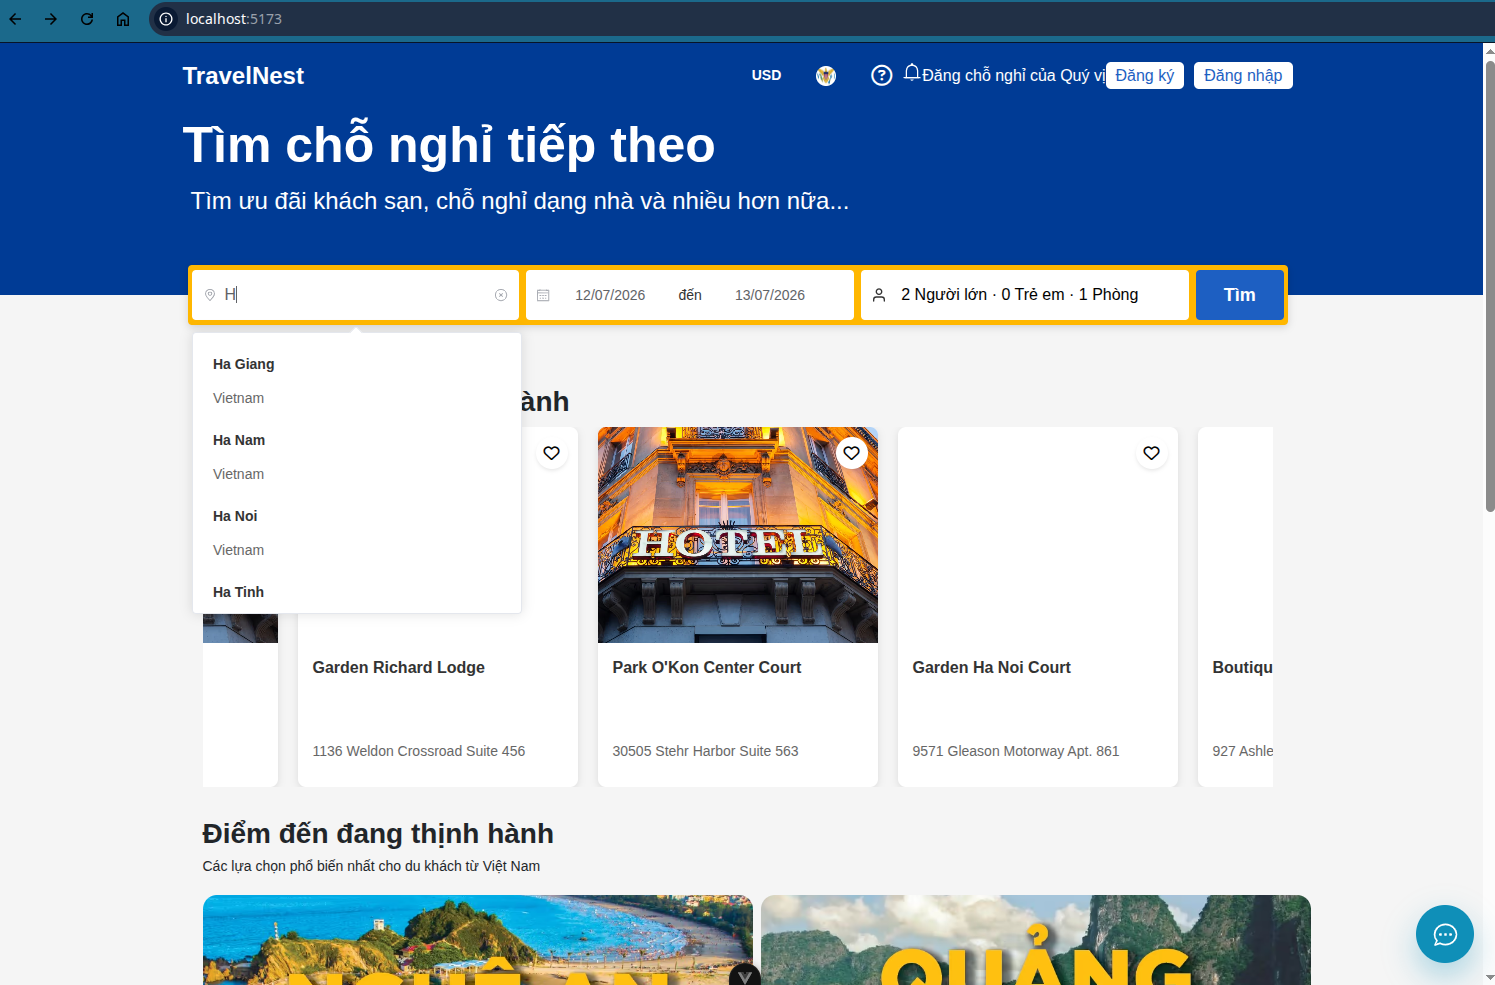
\includegraphics[width=0.95\textwidth]{images/ui_autocomplete.png}
  \caption{Giao diện gợi ý địa điểm khi tìm kiếm (Completion Suggester)}
  \label{fig:ui_autocomplete}
\end{figure}

Hình \ref{fig:ui_autocomplete} minh họa tính năng gợi ý địa điểm (autocomplete) sử dụng Elasticsearch Completion Suggester. Khi người dùng nhập vài ký tự, hệ thống lập tức gợi ý các địa điểm phù hợp trong thời gian thực.

\begin{figure}[H]
  \centering
  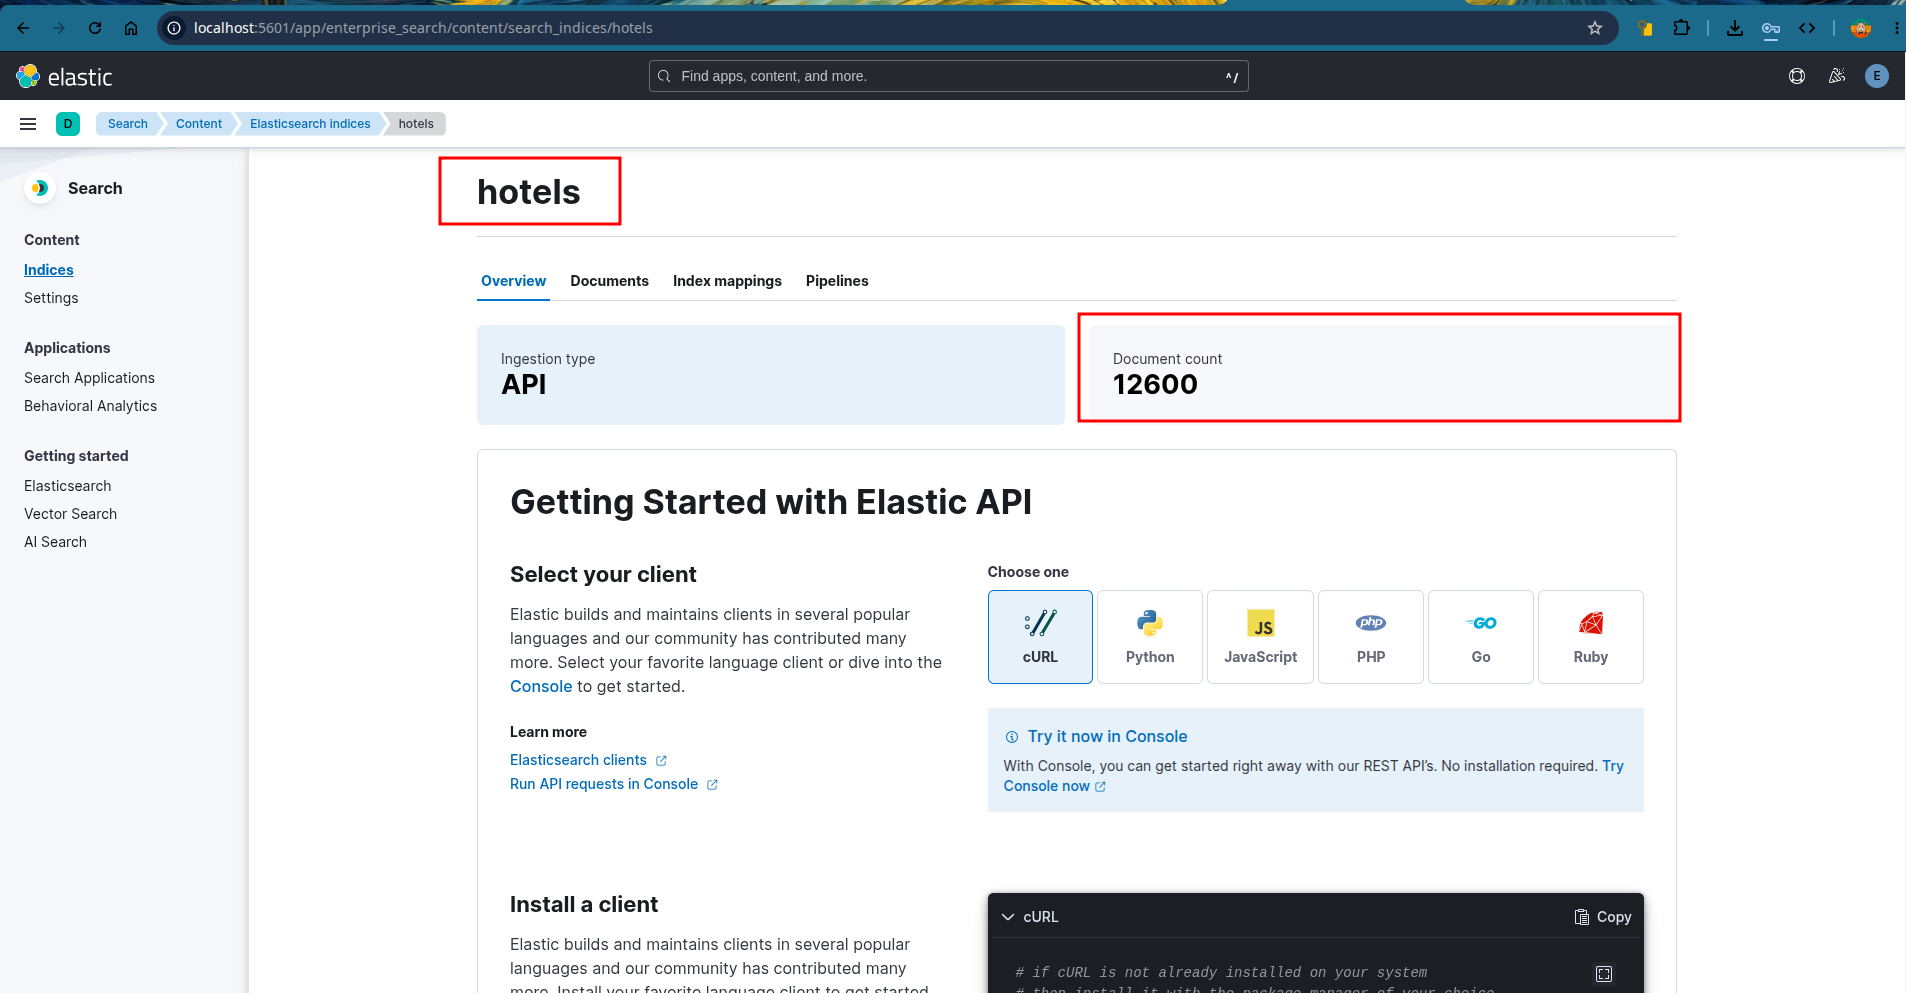
\includegraphics[width=0.95\textwidth]{images/ui_kibana_hotels.png}
  \caption{Giao diện Kibana -- xem chỉ mục (index) khách sạn trong Elasticsearch}
  \label{fig:ui_kibana}
\end{figure}

Hình \ref{fig:ui_kibana} hiển thị giao diện Kibana Dashboard, nơi quản trị viên có thể theo dõi các chỉ mục Elasticsearch, xem dữ liệu khách sạn đã được lập chỉ mục, và giám sát hoạt động tìm kiếm của hệ thống.

\subsection{MongoDB --- Lưu trữ sự kiện phân tích}

MongoDB là cơ sở dữ liệu NoSQL dạng document, lưu trữ dữ liệu dưới dạng JSON-like documents (BSON). Analytics Service (Go) sử dụng MongoDB để lưu trữ SearchLog và HotelViewEvent --- những dữ liệu có cấu trúc linh hoạt và không yêu cầu tính toàn vẹn quan hệ chặt chẽ.

\subsection{MinIO --- Lưu trữ đối tượng (Object Storage)}

MinIO là giải pháp lưu trữ đối tượng (object storage) mã nguồn mở, tương thích với S3 API. TravelNest sử dụng MinIO để lưu trữ ảnh khách sạn, ảnh đánh giá, và các file media khác. Media Service (Go) tương tác với MinIO để upload, download và quản lý ảnh.

Lý do lựa chọn MinIO thay vì AWS S3 trực tiếp:

\begin{itemize}
  \item MinIO có thể được triển khai on-premise hoặc trong Kubernetes cluster, không phụ thuộc vào nhà cung cấp đám mây.
  \item Chi phí thấp hơn khi tự host.
  \item Tương thích S3 API, có thể dễ dàng chuyển sang AWS S3 trong tương lai nếu cần.
  \item Hiệu năng cao, hỗ trợ replication và erasure coding.
\end{itemize}

\subsection{ClickHouse --- Kho dữ liệu phân tích}

ClickHouse là hệ quản trị cơ sở dữ liệu dạng cột (column-oriented DBMS) mã nguồn mở, được thiết kế cho truy vấn phân tích (OLAP) với hiệu năng cực cao. TravelNest sử dụng ClickHouse để lưu trữ dữ liệu search log với khối lượng lớn, phục vụ cho việc phân tích xu hướng tìm kiếm theo thời gian thực.

\section{Cơ chế xác thực và phân quyền}

\subsection{Passport.js --- OAuth và Session Auth}

Passport.js là middleware xác thực cho Node.js, hỗ trợ hơn 500 chiến lược (strategies) xác thực khác nhau. TravelNest sử dụng Passport với các chiến lược:

\begin{itemize}
  \item \textbf{Local Strategy:} Đăng nhập bằng email và mật khẩu.
  \item \textbf{Google OAuth 2.0:} Đăng nhập bằng tài khoản Google.
  \item \textbf{Twitter OAuth:} Đăng nhập bằng tài khoản Twitter/X.
\end{itemize}

\subsection{Keycloak --- Identity and Access Management (IAM)}

Keycloak là giải pháp IAM mã nguồn mở của Red Hat, cung cấp Single Sign-On (SSO), quản lý người dùng, phân quyền, và bảo mật cho ứng dụng. TravelNest đang trong quá trình di chuyển từ Passport.js sang Keycloak để có một giải pháp xác thực tập trung, hỗ trợ OAuth 2.0, OpenID Connect, SAML 2.0, và quản lý người dùng chuyên nghiệp hơn. Chi tiết về quá trình di chuyển này sẽ được trình bày trong Chương 5.

\begin{figure}[H]
  \centering
  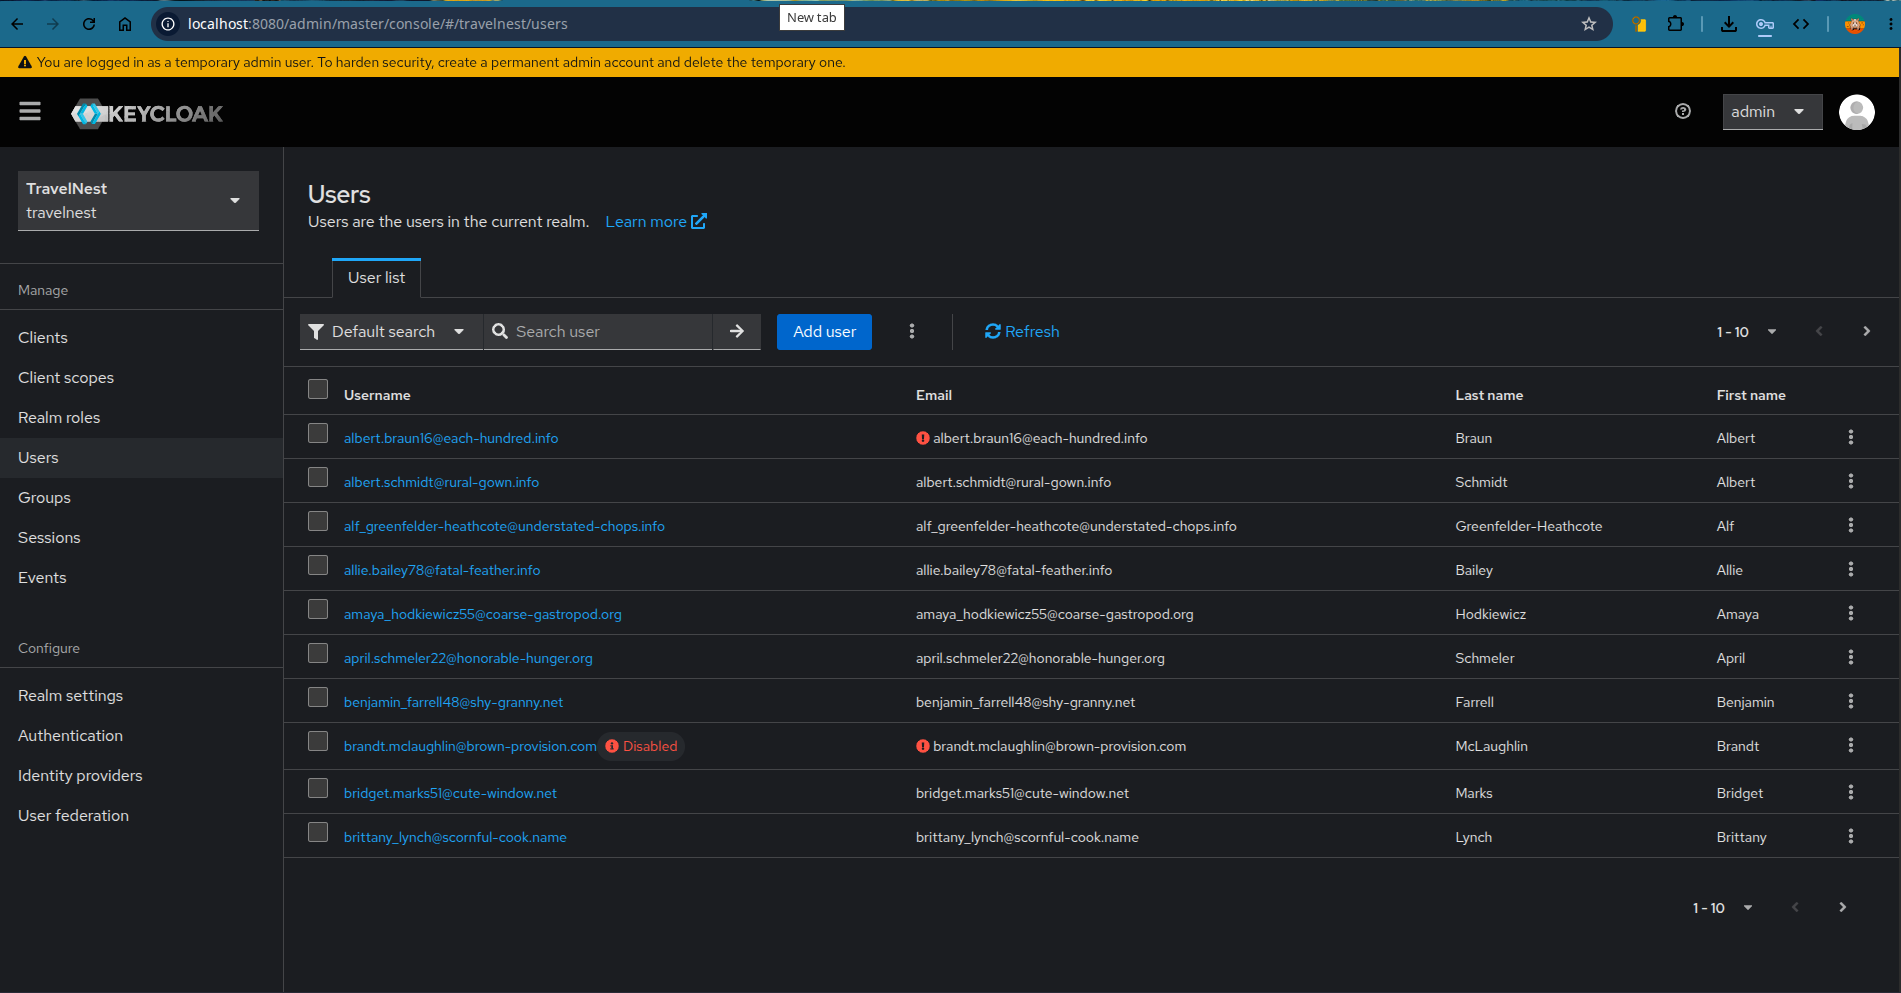
\includegraphics[width=0.95\textwidth]{images/ui_keycloak_users.png}
  \caption{Giao diện quản lý người dùng trên Keycloak Dashboard}
  \label{fig:ui_keycloak}
\end{figure}

Hình \ref{fig:ui_keycloak} hiển thị giao diện quản trị Keycloak, nơi quản trị viên hệ thống có thể quản lý tập trung tất cả người dùng, vai trò, và phân quyền trên toàn bộ hệ thống TravelNest.

\section{Tích hợp thanh toán --- Stripe}

Stripe là nền tảng thanh toán trực tuyến hàng đầu thế giới, cung cấp API cho phép xử lý thanh toán, quản lý khách hàng, và tự động hóa quy trình tài chính. TravelNest tích hợp Stripe để xử lý các giao dịch thanh toán đặt phòng \cite{stripe2024docs}.

Lý do lựa chọn Stripe thay vì PayPal hoặc VNPay:

\begin{itemize}
  \item API của Stripe được thiết kế tốt, dễ tích hợp, tài liệu chi tiết và có thư viện SDK cho Node.js.
  \item Hỗ trợ webhook để nhận thông báo real-time về trạng thái thanh toán.
  \item Hỗ trợ đầy đủ các nghiệp vụ: Payment Intent, Refund, Payout, và Connect (cho marketplace).
  \item Stripe Elements cung cấp UI components tùy chỉnh được, đảm bảo trải nghiệm thanh toán liền mạch.
  \item Hỗ trợ nhiều loại thẻ và phương thức thanh toán quốc tế.
  \item PCI-DSS Level 1 compliant, đảm bảo an toàn dữ liệu thẻ tín dụng.
\end{itemize}

\begin{figure}[H]
  \centering
  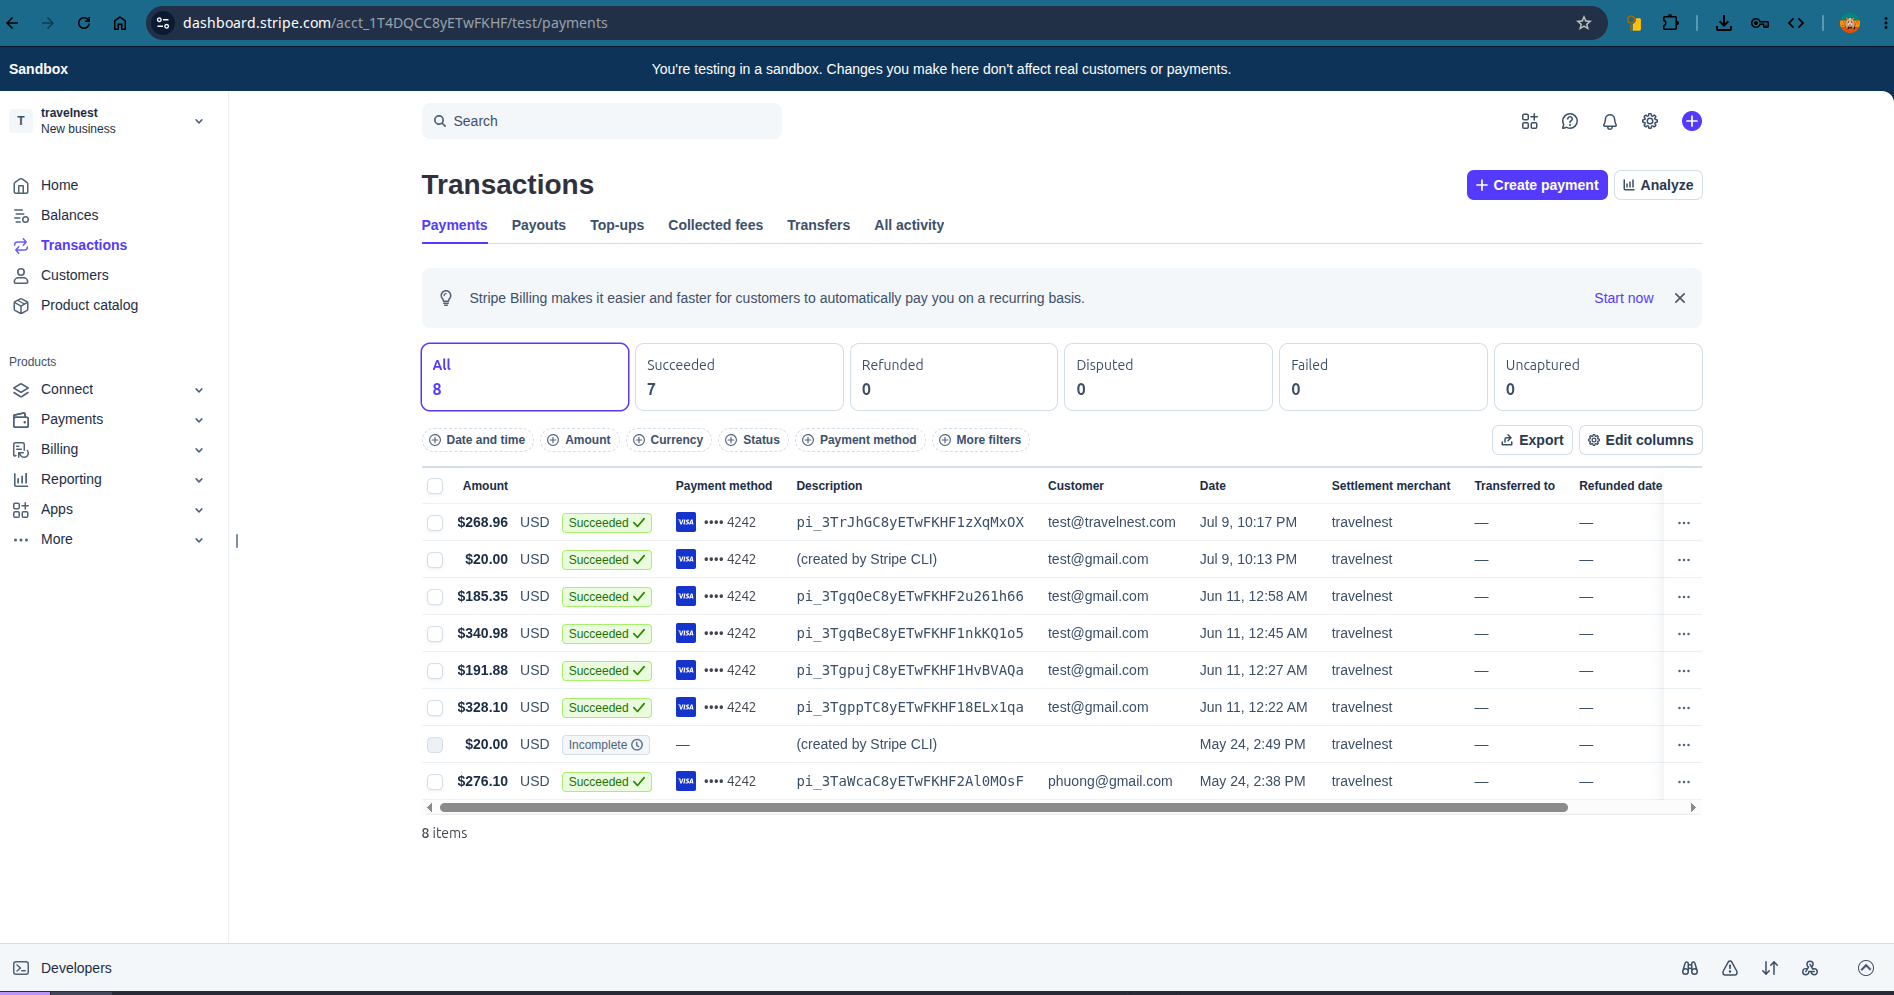
\includegraphics[width=0.95\textwidth]{images/ui_stripe_dashboard.png}
  \caption{Giao diện Stripe Dashboard -- quản lý giao dịch thanh toán}
  \label{fig:ui_stripe}
\end{figure}

Hình \ref{fig:ui_stripe} hiển thị bảng điều khiển Stripe, nơi quản trị viên có thể theo dõi tất cả các giao dịch thanh toán, hoàn tiền và chi trả được xử lý qua hệ thống TravelNest.

\section{Công nghệ triển khai và DevOps}

\subsection{Docker và Kubernetes}

Docker là nền tảng containerization phổ biến nhất, cho phép đóng gói ứng dụng cùng toàn bộ môi trường thành một container độc lập, đảm bảo tính nhất quán giữa môi trường phát triển và production.

Kubernetes (K8s) là hệ thống điều phối container (container orchestration), tự động hóa việc triển khai, mở rộng và quản lý các ứng dụng containerized \cite{kubernetes2024docs}. TravelNest triển khai trên một cụm Kubernetes (k3s) với 7 ứng dụng chạy song song: API server, Frontend, Admin Client, BullMQ Worker, Analytics Service, Media Service, và Notification Service.

\subsection{Argo CD --- GitOps}

Argo CD là công cụ triển khai GitOps cho Kubernetes, cho phép đồng bộ trạng thái thực tế của cluster với trạng thái mong muốn được định nghĩa trong Git repository \cite{argocd2024docs}. Trong TravelNest, tất cả các manifest Kubernetes (deployment, service, configmap, ingress) được lưu trong thư mục \texttt{deploy/k8s/}. Argo CD tự động phát hiện thay đổi và đồng bộ, đảm bảo mọi thay đổi đều có thể truy vết và rollback dễ dàng.

\subsection{GitHub Actions --- CI/CD}

GitHub Actions là dịch vụ CI/CD tích hợp sẵn trong GitHub, cho phép tự động hóa quy trình build, test và deploy. TravelNest có 6 workflow GitHub Actions riêng biệt cho backend, frontend, admin-client, analytics-service, media-service, và notification-service. Mỗi workflow bao gồm các bước:

\begin{enumerate}
  \item Lint code (ESLint, Prettier cho JavaScript; gofmt, golangci-lint cho Go).
  \item Chạy unit test và integration test.
  \item Build Docker image.
  \item Push Docker image lên container registry.
  \item Cập nhật manifest trong Git repository (cho Argo CD đồng bộ).
\end{enumerate}

\subsection{Giao tiếp thời gian thực --- Socket.IO}

Socket.IO là thư viện cho phép giao tiếp hai chiều, real-time giữa client và server dựa trên WebSocket, với cơ chế fallback tự động (long polling) khi WebSocket không khả dụng. TravelNest sử dụng Socket.IO để:

\begin{itemize}
  \item Gửi thông báo real-time cho người dùng (xác nhận đặt phòng, nhắc nhở check-in).
  \item Cập nhật tình trạng phòng trống real-time trên trang chi tiết khách sạn.
  \item Gửi cảnh báo cho chủ khách sạn khi có đơn đặt mới.
\end{itemize}

\section{Bảng tổng hợp công nghệ}

Bảng \ref{tab:tech_stack} tổng hợp toàn bộ các công nghệ được sử dụng trong hệ thống TravelNest.

\begin{table}[H]
  \centering
  \caption{Tổng hợp công nghệ sử dụng trong TravelNest}
  \label{tab:tech_stack}
  \begin{tabularx}{\textwidth}{p{3.5cm} p{3.5cm} X}
    \toprule
    \textbf{Lớp} & \textbf{Công nghệ} & \textbf{Vai trò} \\
    \midrule
    Frontend (User) & Vue 3, Vite, Element Plus, Leaflet, Vuex, Chart.js, Socket.IO Client & Giao diện người dùng cho khách hàng \\
    Frontend (Admin) & Nuxt 4, Pinia, Tailwind CSS, TypeScript & Bảng điều khiển quản trị cho chủ khách sạn \\
    Backend API & Node.js 18+, Express.js, Sequelize ORM & Xử lý nghiệp vụ lõi, REST API \\
    Background Jobs & BullMQ, Redis & Xử lý tác vụ bất đồng bộ \\
    Microservices & Go 1.22, NATS JetStream & Analytics, Media, Notification \\
    Database & MySQL 8.0 & Lưu trữ dữ liệu giao dịch \\
    Caching \& Queue & Redis 7 & Session store, caching, rate limiting, BullMQ backend \\
    Search Engine & Elasticsearch 8.11 & Tìm kiếm toàn văn, gợi ý địa điểm \\
    Analytics DB & MongoDB, ClickHouse & Lưu trữ và phân tích sự kiện \\
    Object Storage & MinIO (S3-compatible) & Lưu trữ ảnh và media \\
    Event Bus & NATS JetStream & Giao tiếp bất đồng bộ giữa các service \\
    Auth & Passport.js, Keycloak (đang chuyển đổi) & Xác thực và phân quyền \\
    Payment & Stripe & Xử lý thanh toán trực tuyến \\
    Notifications & Nodemailer, Infobip (SMS), Socket.IO & Gửi thông báo đa kênh \\
    Deployment & Docker, Kubernetes (k3s), Argo CD, Cloudflare Tunnel & Container hóa và triển khai \\
    CI/CD & GitHub Actions & Tự động hóa build, test, deploy \\
    Monitoring & Elasticsearch, Kibana & Log aggregation và giám sát \\
    \bottomrule
  \end{tabularx}
\end{table}

Chương này đã trình bày chi tiết các công nghệ và nền tảng lý thuyết được sử dụng trong quá trình phát triển hệ thống TravelNest. Với mỗi công nghệ, em đã phân tích lý do lựa chọn và so sánh với các giải pháp thay thế, nhằm đảm bảo sự phù hợp với yêu cầu của hệ thống. Trong chương tiếp theo, chúng ta sẽ áp dụng các công nghệ này vào quá trình phân tích thiết kế và triển khai hệ thống TravelNest.


% ============================================================================
% CHƯƠNG 4: PHÂN TÍCH THIẾT KẾ, TRIỂN KHAI VÀ ĐÁNH GIÁ HỆ THỐNG
% ============================================================================
\chapter{PHÂN TÍCH THIẾT KẾ, TRIỂN KHAI VÀ ĐÁNH GIÁ HỆ THỐNG}

Chương 3 đã thảo luận về các công nghệ và nền tảng lý thuyết được lựa chọn để xây dựng hệ thống TravelNest. Chương này sẽ áp dụng các công nghệ đó vào quá trình phân tích, thiết kế, triển khai và đánh giá hệ thống. Chúng ta sẽ đi từ kiến trúc tổng quan đến thiết kế chi tiết từng thành phần, từ cơ sở dữ liệu đến giao diện người dùng, và cuối cùng là quy trình triển khai trên môi trường production.

\section{Thiết kế kiến trúc}

\subsection{Lựa chọn kiến trúc phần mềm}

TravelNest áp dụng kiến trúc \textbf{hybrid monolith-microservice}, kết hợp giữa mô hình MVC cho khối monolithic (Node.js backend) và mô hình event-driven cho các microservice (Go). Đây là một biến thể của chiến lược \textit{Strangler Fig Pattern} --- một chiến lược di chuyển từ monolithic sang microservice bằng cách thay thế dần từng thành phần.

Trong giai đoạn hiện tại, kiến trúc của TravelNest được tổ chức như sau:

\begin{itemize}
  \item \textbf{API Gateway / Monolithic Core (Node.js):} Đảm nhận tất cả các nghiệp vụ lõi --- xác thực, quản lý khách sạn, đặt phòng, thanh toán, đánh giá --- và phục vụ các API endpoint cho cả client và admin. Backend tuân thủ mô hình MVC phân lớp: Routes \texttt{->} Controllers \texttt{->} Services \texttt{->} Repositories \texttt{->} Models (Sequelize).
  \item \textbf{Event Bus (NATS JetStream):} Là lớp trung gian cho phép monolithic core publish các domain events và Go microservices consume một cách bất đồng bộ.
  \item \textbf{Go Microservices:} Ba dịch vụ được tách ra khỏi monolith --- Analytics, Media, Notification --- mỗi dịch vụ có cơ sở dữ liệu riêng và giao tiếp qua NATS.
  \item \textbf{Background Workers (BullMQ):} Xử lý các tác vụ nền trong phạm vi monolith, bao gồm đồng bộ Elasticsearch, hết hạn giữ chỗ, và hết hạn đặt phòng.
  \item \textbf{Infrastructure Layer:} Bao gồm MySQL, Redis, Elasticsearch, MongoDB, MinIO, ClickHouse, và NATS.
\end{itemize}

\begin{figure}[H]
  \centering
  % PLACEHOLDER: Biểu đồ kiến trúc tổng quan
  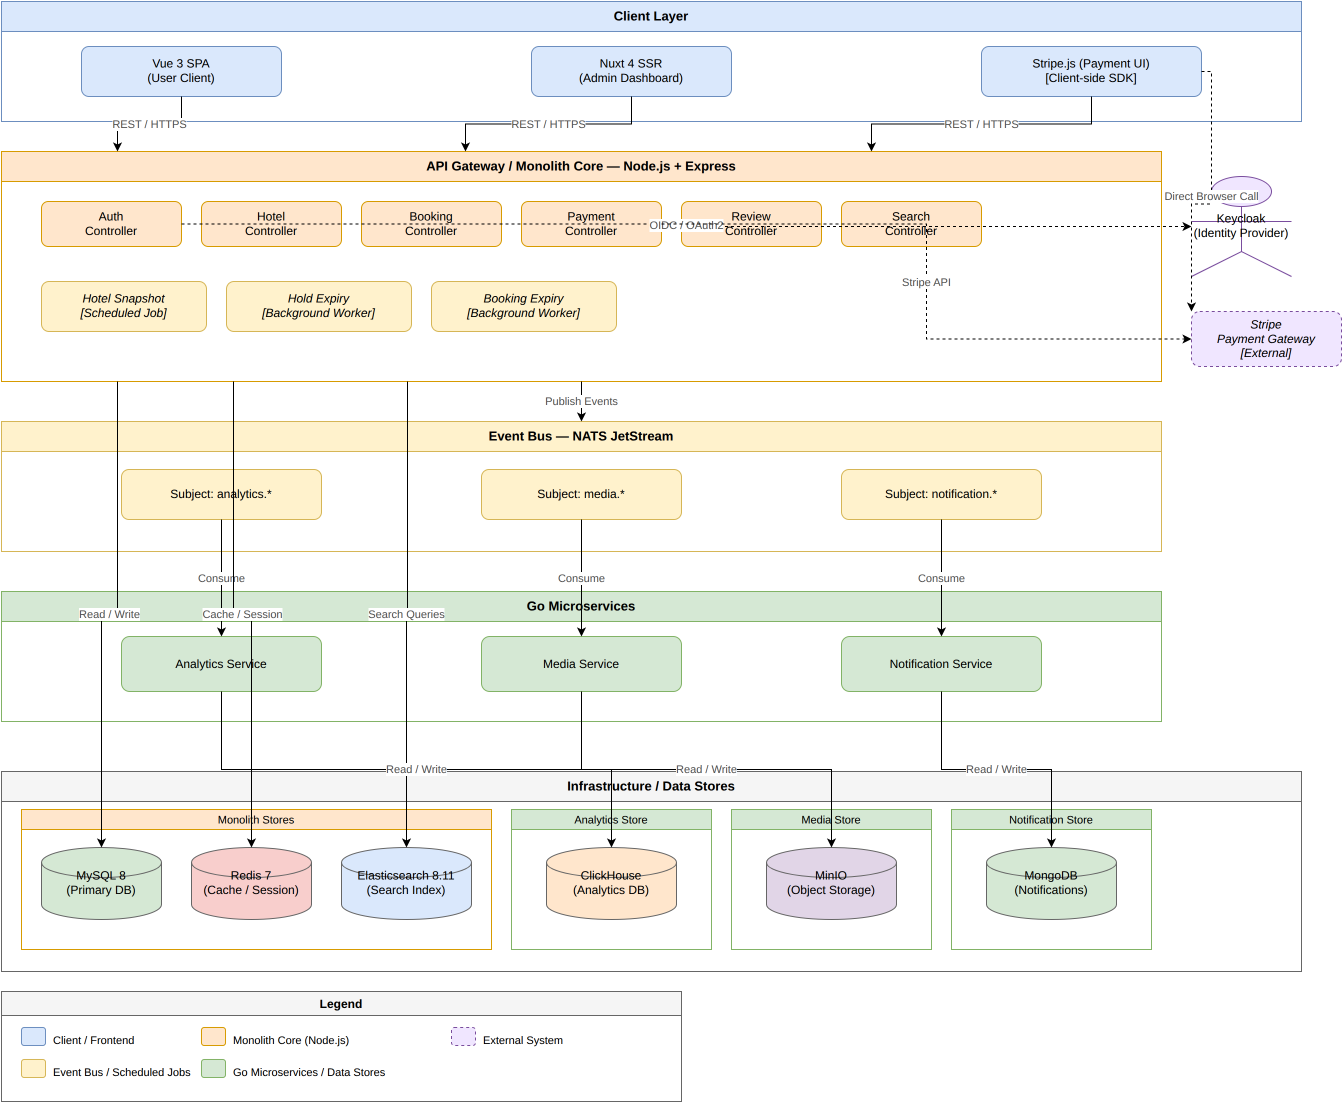
\includegraphics[width=0.95\textwidth]{images/fig_4_1_architecture.png}
  \caption{Kiến trúc tổng quan hệ thống TravelNest}
  \label{fig:architecture_overview}
\end{figure}

Hình \ref{fig:architecture_overview} mô tả kiến trúc tổng quan của TravelNest, bao gồm luồng dữ liệu chính: (1) Người dùng truy cập client qua trình duyệt; (2) Client gửi yêu cầu đến Node.js API thông qua HTTPS; (3) API tương tác với MySQL để xử lý nghiệp vụ; (4) API publish events lên NATS; (5) Go services consume events và xử lý bất đồng bộ; (6) API truy vấn Elasticsearch cho tìm kiếm; (7) Redis được sử dụng cho session store và caching.

\subsection{Thiết kế tổng quan}

Hình \ref{fig:package_diagram} mô tả biểu đồ gói (UML package diagram) cho khối backend Node.js, thể hiện sự phụ thuộc giữa các gói chính.

\begin{figure}[H]
  \centering
  % PLACEHOLDER: Biểu đồ gói
  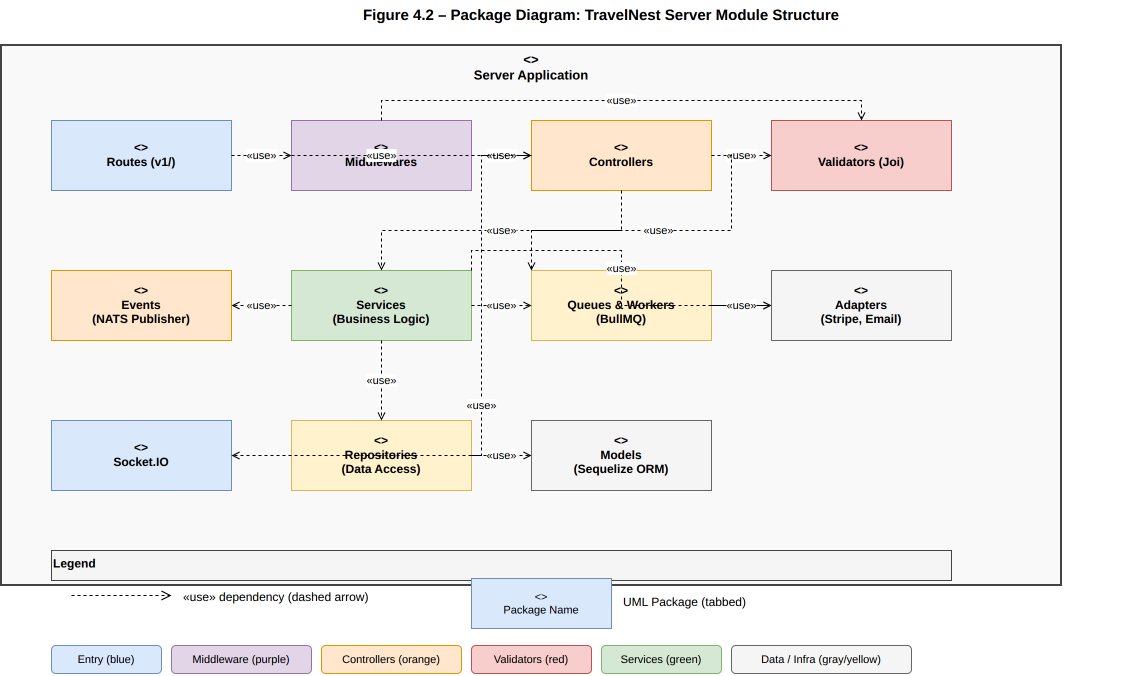
\includegraphics[width=0.95\textwidth]{images/fig_4_2_package_diagram.png}
  \caption{Biểu đồ gói UML của khối backend Node.js}
  \label{fig:package_diagram}
\end{figure}

Kiến trúc phân lớp của backend được tổ chức thành các gói (package) sau, tuân thủ nguyên tắc phụ thuộc một chiều (từ trên xuống):

\begin{enumerate}
  \item \textbf{Routes:} Định nghĩa các HTTP endpoint và phương thức (GET, POST, PUT, DELETE). Các route không chứa business logic, chỉ gọi đến controllers hoặc middleware tương ứng. Ví dụ: \texttt{/api/v1/auth/login}, \texttt{/api/v1/hotels/search}.
  \item \textbf{Middlewares:} Xử lý các tác vụ xuyên suốt (cross-cutting concerns) như xác thực (auth middleware), validation (Joi schema validation), rate limiting, logging, CSRF protection, và error handling.
  \item \textbf{Controllers:} Nhận input từ routes, gọi services, và trả về response. Controllers rất mỏng (thin) --- chỉ tập trung vào việc điều phối, không chứa business logic.
  \item \textbf{Services:} Chứa toàn bộ business logic của hệ thống. Mỗi service tương ứng với một domain (AuthService, BookingService, HotelService, PaymentService, ReviewService, SearchService...). Services gọi repositories để truy xuất dữ liệu và gọi events để publish events lên NATS.
  \item \textbf{Repositories:} Đóng gói các thao tác truy xuất dữ liệu với Sequelize models. Mỗi repository tương ứng với một hoặc một nhóm models liên quan, cung cấp các phương thức CRUD và query phức tạp.
  \item \textbf{Models:} Định nghĩa cấu trúc bảng MySQL thông qua Sequelize, bao gồm schema, associations, hooks, và validation. Có 47 models trong hệ thống.
  \item \textbf{Events:} Module phụ trách việc publish domain events lên NATS JetStream. Mỗi loại event (analytics, media, notification) có một publisher riêng.
  \item \textbf{Queues \& Workers:} Định nghĩa các queue BullMQ và worker tương ứng để xử lý tác vụ nền.
  \item \textbf{Adapters:} Tích hợp với các dịch vụ bên ngoài như Stripe (thanh toán), Nodemailer (email), và Infobip (SMS).
  \item \textbf{Socket:} Quản lý kết nối Socket.IO và điều phối các sự kiện real-time.
\end{enumerate}

\subsection{Thiết kế chi tiết gói}

Trong số các gói nghiệp vụ (Auth, Booking, Hotel, Payment, Review, Search), phần này trình bày chi tiết thiết kế của hai gói Auth và Booking như hai ví dụ tiêu biểu, đại diện cho nhóm chức năng xác thực/bảo mật và nhóm chức năng nghiệp vụ lõi (đặt phòng, giữ chỗ, thanh toán); các gói còn lại được thiết kế theo cùng nguyên tắc phân tầng Routes -- Middlewares -- Controllers -- Services -- Repositories -- Models đã trình bày ở trên.

\subsubsection{Gói Auth}

Hình \ref{fig:package_auth} mô tả thiết kế chi tiết của gói Auth, bao gồm các lớp và mối quan hệ giữa chúng.

\begin{figure}[H]
  \centering
  % PLACEHOLDER: Thiết kế gói Auth
  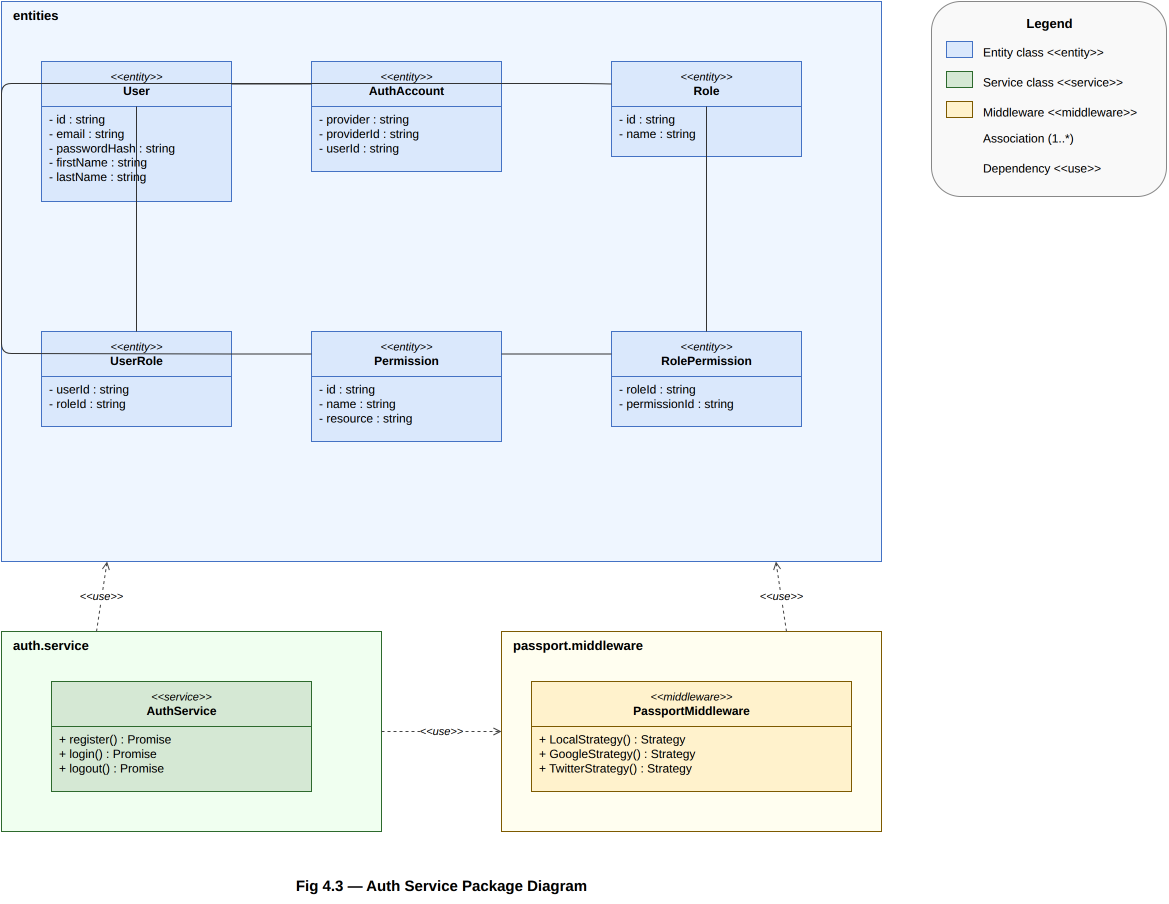
\includegraphics[width=0.95\textwidth]{images/fig_4_3_auth_package.png}
  \caption{Thiết kế chi tiết gói Auth}
  \label{fig:package_auth}
\end{figure}

Gói Auth quản lý toàn bộ quá trình xác thực và phân quyền của hệ thống. Các thành phần chính bao gồm:

\begin{itemize}
  \item \textbf{User Model:} Đại diện cho người dùng với các thuộc tính: id, email, password (đã hash), firstName, lastName, phone, avatar, status.
  \item \textbf{AuthAccount Model:} Liên kết người dùng với các phương thức xác thực bên ngoài (Google, Twitter) thông qua provider và providerId.
  \item \textbf{Role và Permission Models:} Hệ thống phân quyền dựa trên vai trò (RBAC). Mỗi người dùng có một hoặc nhiều vai trò (Guest, HotelAdmin, SystemAdmin), mỗi vai trò có nhiều quyền (permission).
  \item \textbf{AuthService:} Xử lý logic đăng ký, đăng nhập (local + OAuth), quản lý session, và reset password.
  \item \textbf{Passport Middleware:} Tích hợp Passport.js với các chiến lược Local, Google, và Twitter.
\end{itemize}

\subsubsection{Gói Booking}

Hình \ref{fig:package_booking} mô tả thiết kế chi tiết của gói Booking --- gói phức tạp nhất trong hệ thống.

\begin{figure}[H]
  \centering
  % PLACEHOLDER: Thiết kế gói Booking
  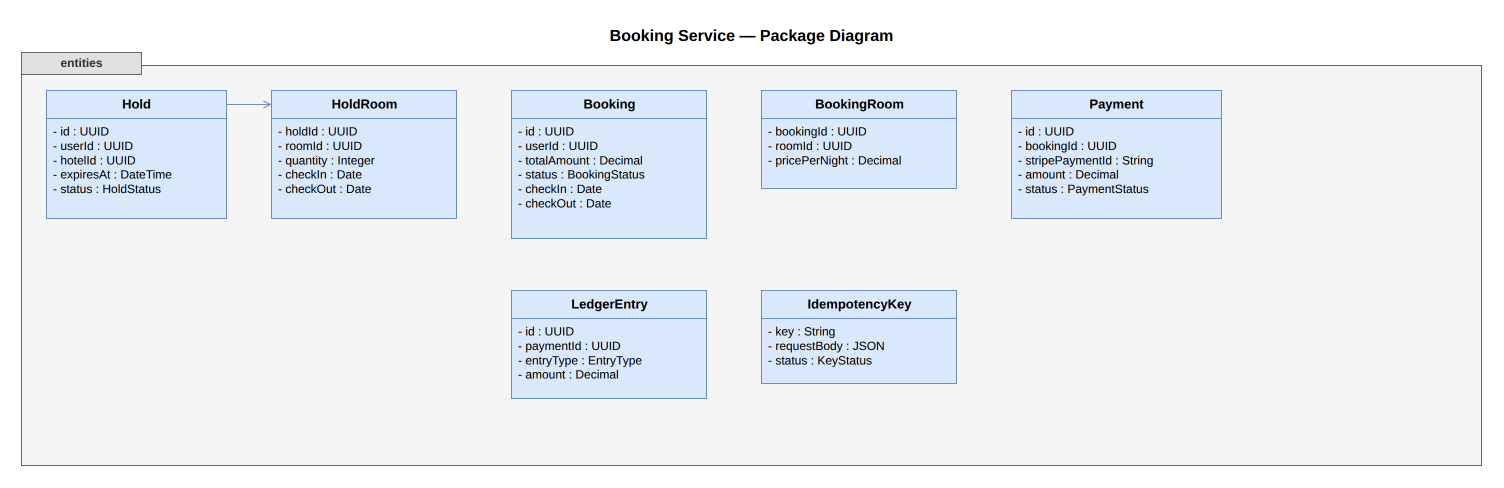
\includegraphics[width=0.95\textwidth]{images/fig_4_4_booking_package.png}
  \caption{Thiết kế chi tiết gói Booking}
  \label{fig:package_booking}
\end{figure}

Gói Booking bao gồm ba quy trình chính: Giữ chỗ (Hold), Đặt phòng (Booking), và Thanh toán (Payment). Các thành phần:

\begin{itemize}
  \item \textbf{HoldService:} Tạo bản ghi giữ chỗ tạm thời (15 phút), kiểm tra tình trạng phòng trống, và tự động hủy khi hết hạn (qua BullMQ worker).
  \item \textbf{BookingService:} Chuyển đổi Hold thành Booking sau khi thanh toán thành công, cập nhật RoomInventory, và gửi sự kiện đến NATS.
  \item \textbf{PaymentService:} Tương tác với Stripe API để tạo Payment Intent, xử lý webhook từ Stripe, và cập nhật trạng thái thanh toán.
  \item \textbf{LedgerService:} Quản lý sổ cái kép (double-entry ledger): mỗi giao dịch (thanh toán, hoàn tiền, chi trả cho chủ khách sạn) được ghi thành hai bút toán (debit và credit) trong LedgerEntry, đảm bảo cân bằng tài khoản.
  \item \textbf{Booking Model:} Lưu trữ thông tin đặt phòng với các trạng thái: Pending, Confirmed, CheckedIn, Completed, Cancelled.
  \item \textbf{Hold Model:} Lưu trữ giữ chỗ tạm thời với thời gian hết hạn (expiresAt).
  \item \textbf{Payment, Refund, Payout, Transaction Models:} Lưu trữ lịch sử giao dịch tài chính.
  \item \textbf{IdempotencyKey Model:} Đảm bảo mỗi yêu cầu thanh toán chỉ được xử lý đúng một lần, tránh trùng lặp khi webhook từ Stripe được gửi nhiều lần.
\end{itemize}

\section{Thiết kế chi tiết}

\subsection{Thiết kế giao diện}

Hệ thống TravelNest có hai giao diện riêng biệt cho hai nhóm người dùng chính.

\subsubsection{Giao diện khách hàng (Vue 3 SPA)}

Giao diện khách hàng là một Single Page Application (SPA) được xây dựng bằng Vue 3 và Vite. Các trang chính bao gồm:

\begin{itemize}
  \item \textbf{Trang chủ (Home):} Hiển thị thanh tìm kiếm lớn với ô nhập điểm đến, chọn ngày, số khách, cùng danh sách khách sạn nổi bật và điểm đến phổ biến (Hình \ref{fig:ui_home}).
  \item \textbf{Trang kết quả tìm kiếm (Search Results):} Hiển thị danh sách khách sạn dưới dạng card, kèm bộ lọc (giá, đánh giá, tiện nghi) và bản đồ tương tác hiển thị vị trí khách sạn.
  \item \textbf{Trang chi tiết khách sạn (Hotel Detail):} Hiển thị đầy đủ thông tin: ảnh, mô tả, tiện nghi, chính sách, các loại phòng với giá tương ứng theo ngày đã chọn, đánh giá từ khách hàng trước.
  \item \textbf{Trang thanh toán (Checkout):} Tóm tắt đơn đặt, form nhập thông tin khách, và tích hợp Stripe Elements để nhập thông tin thẻ.
  \item \textbf{Trang quản lý đơn đặt (My Bookings):} Danh sách các đơn đặt của người dùng với trạng thái và các hành động (xem chi tiết, hủy, viết đánh giá).
\end{itemize}

\begin{figure}[H]
  \centering
  % PLACEHOLDER: Giao diện trang chủ
  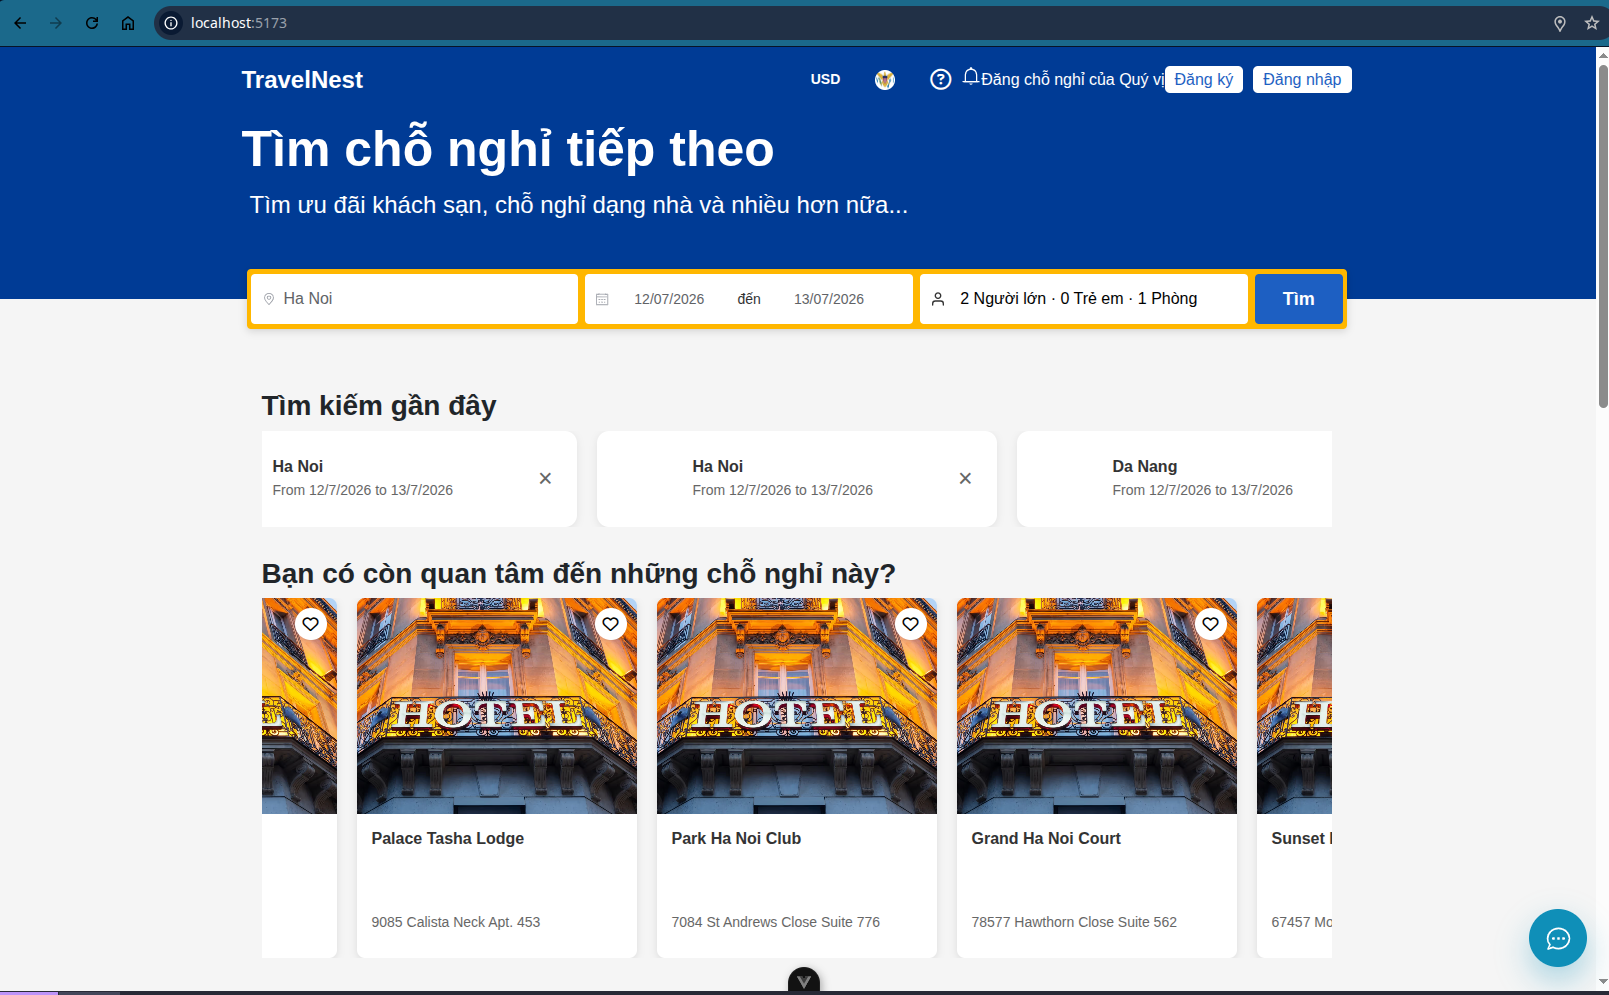
\includegraphics[width=0.95\textwidth]{images/ui_home.png}
  \caption{Giao diện trang chủ TravelNest (client)}
  \label{fig:ui_home}
\end{figure}

Giao diện được thiết kế theo phong cách hiện đại, tối giản (clean), lấy cảm hứng từ Booking.com. Bố cục responsive, sử dụng Element Plus components để đảm bảo tính nhất quán. Ngôn ngữ giao diện hỗ trợ tiếng Việt và tiếng Anh, tự động chuyển đổi dựa trên cài đặt trình duyệt hoặc lựa chọn của người dùng.

\begin{figure}[H]
  \centering
  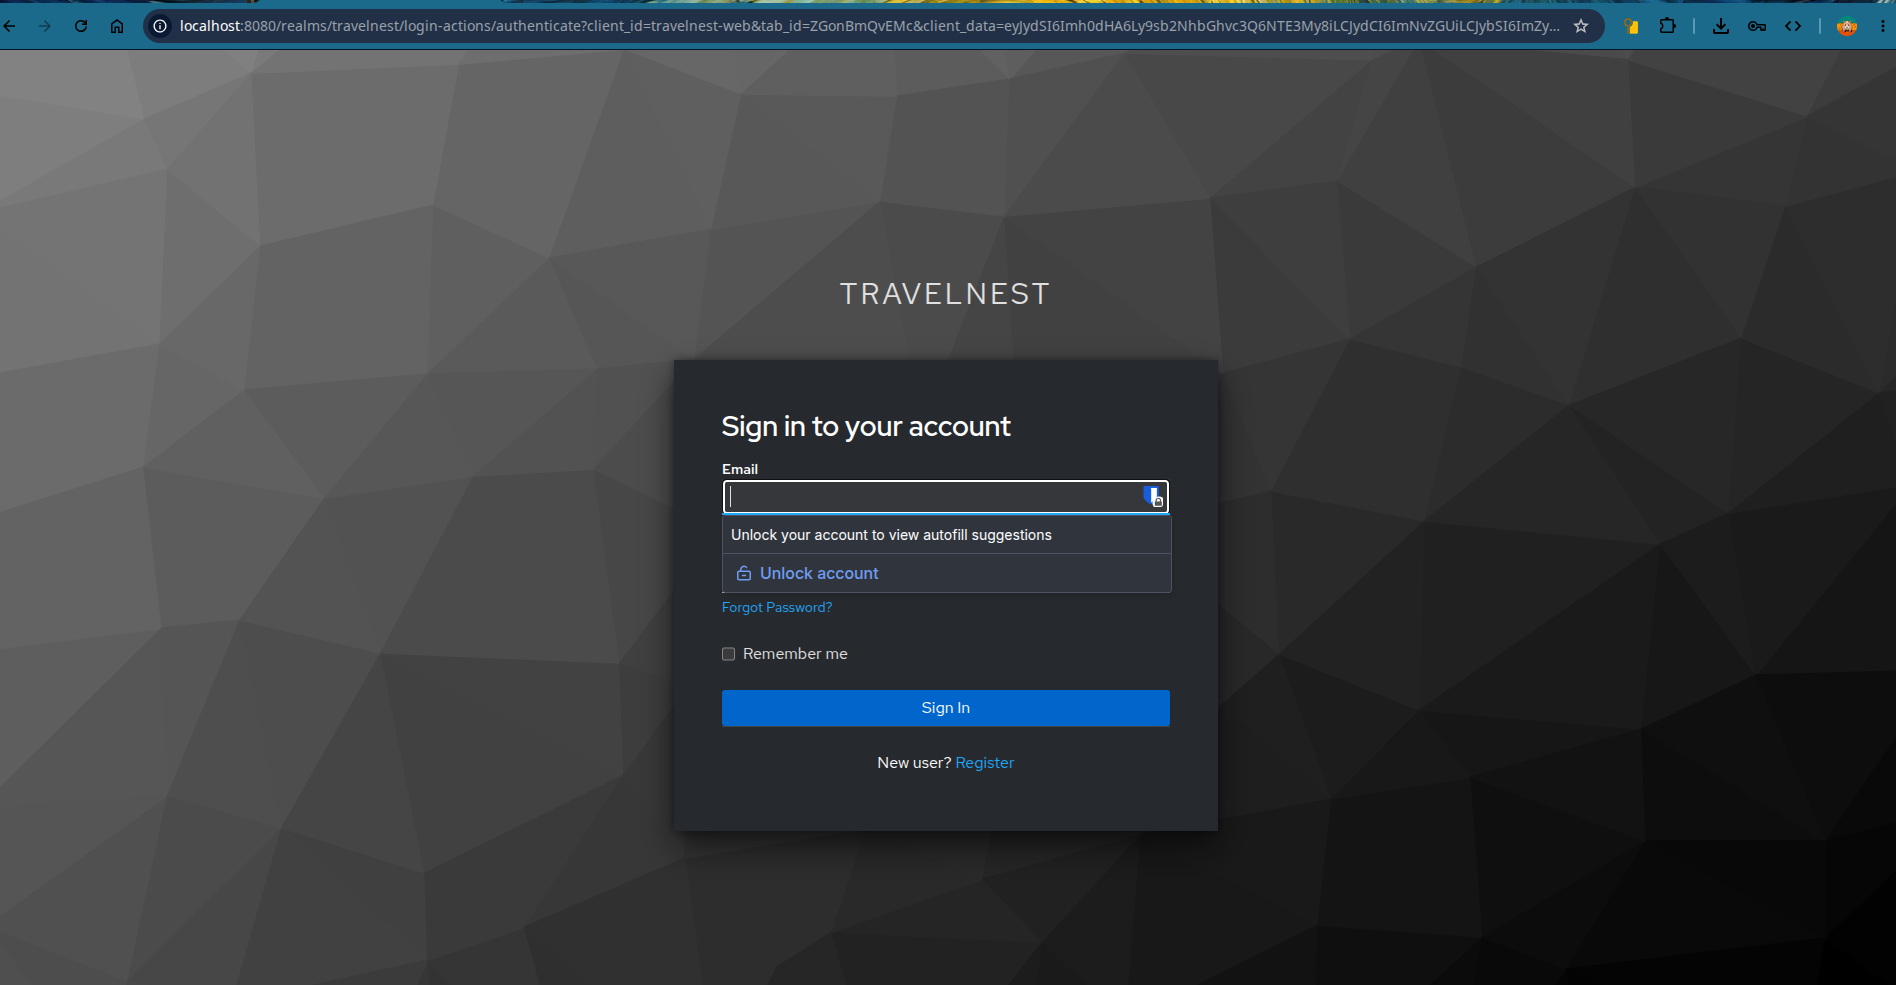
\includegraphics[width=0.95\textwidth]{images/ui_login.png}
  \caption{Giao diện trang đăng nhập}
  \label{fig:ui_login}
\end{figure}

Hình \ref{fig:ui_login} hiển thị trang đăng nhập của TravelNest, hỗ trợ đăng nhập qua email/mật khẩu hoặc thông qua các tài khoản mạng xã hội (Google, Twitter).

\begin{figure}[H]
  \centering
  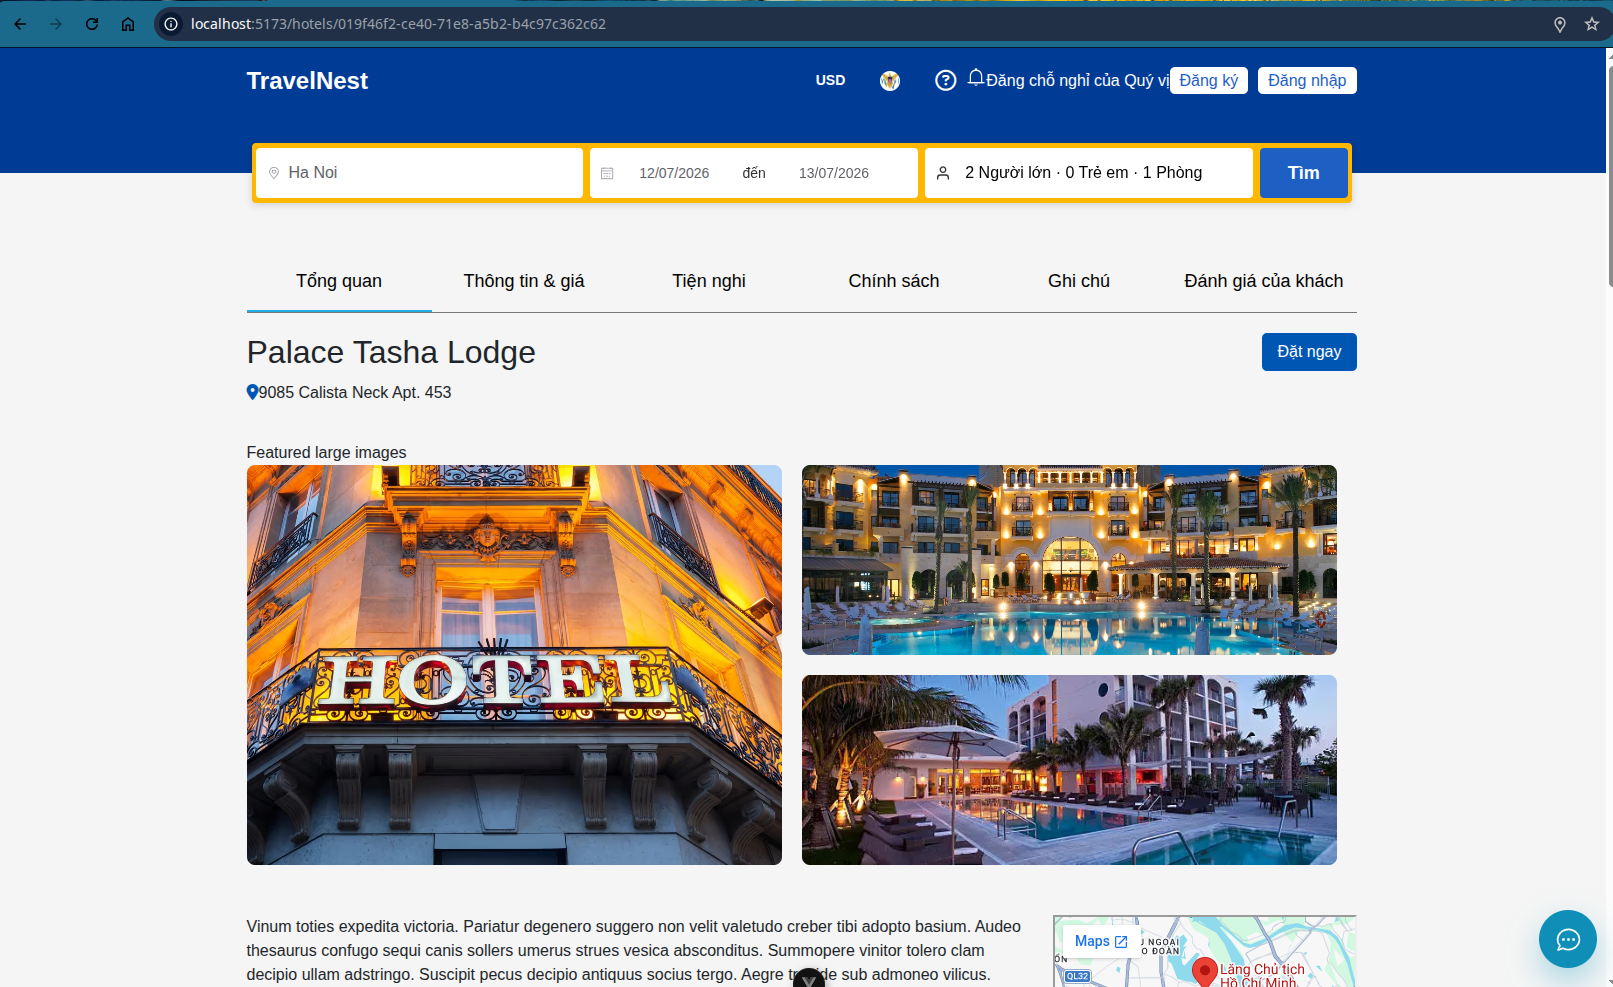
\includegraphics[width=0.95\textwidth]{images/ui_hotel_detail.png}
  \caption{Giao diện trang chi tiết khách sạn}
  \label{fig:ui_hotel_detail}
\end{figure}

Hình \ref{fig:ui_hotel_detail} minh họa trang chi tiết khách sạn, nơi người dùng có thể xem đầy đủ thông tin về khách sạn, các loại phòng với giá tương ứng, tiện nghi, chính sách và đánh giá từ khách hàng trước đó.

\begin{figure}[H]
  \centering
  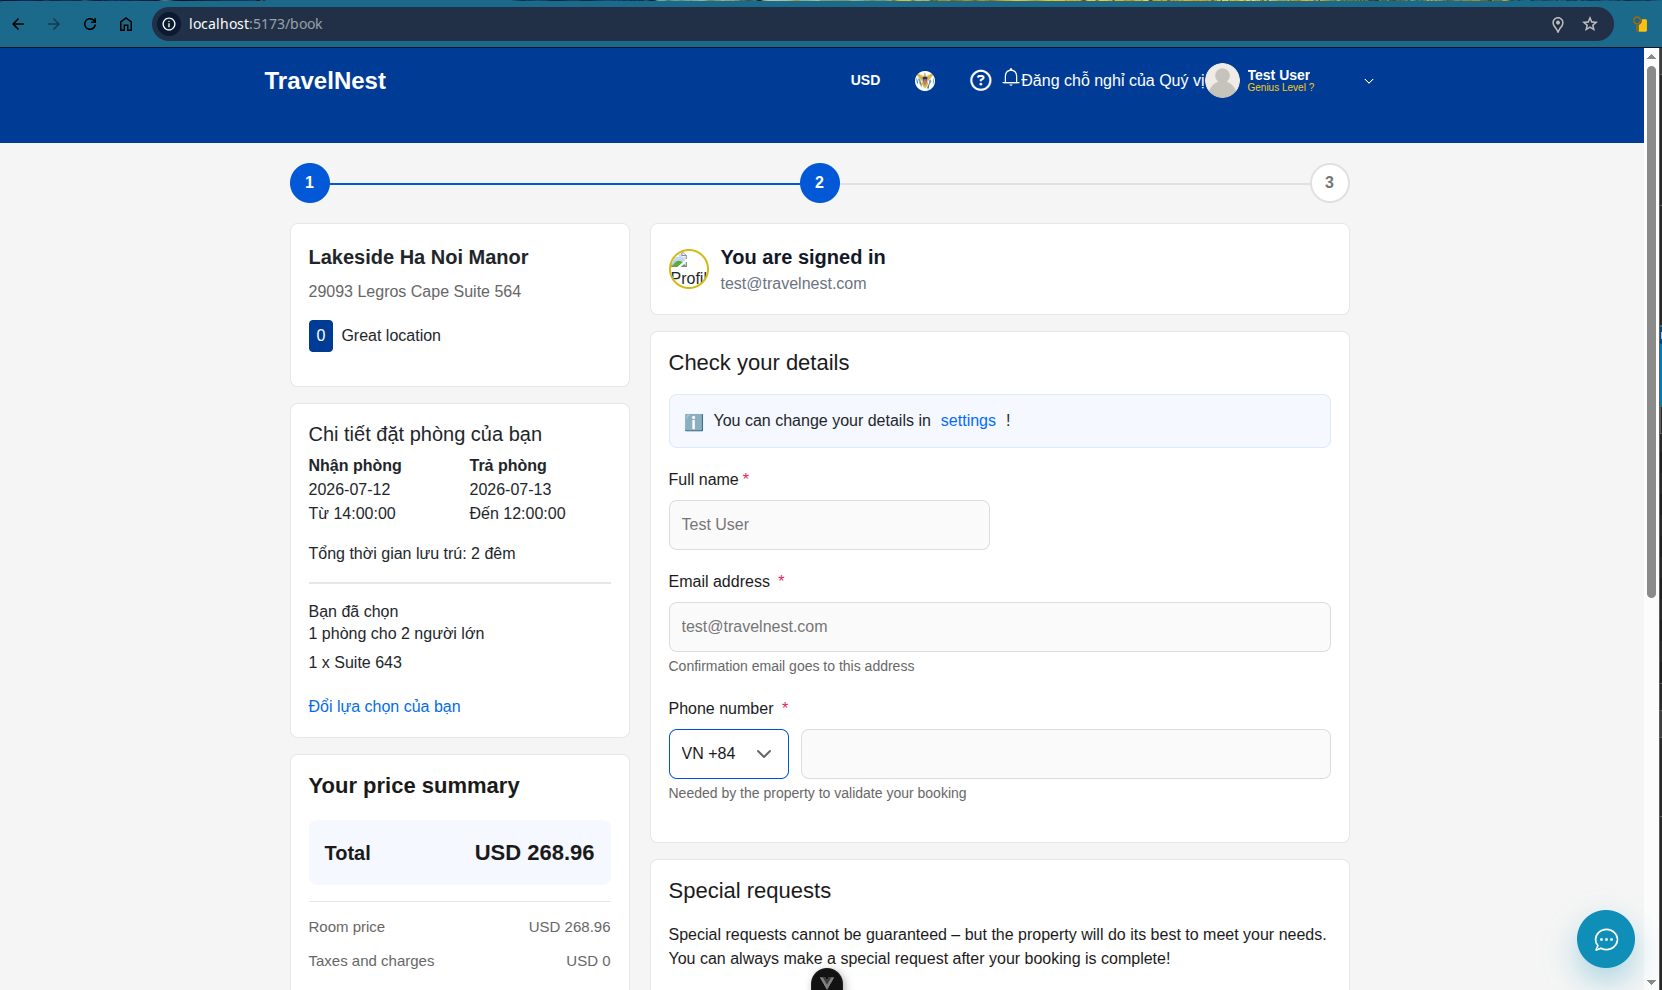
\includegraphics[width=0.95\textwidth]{images/ui_checkout.png}
  \caption{Giao diện trang thanh toán -- tóm tắt đơn đặt}
  \label{fig:ui_checkout}
\end{figure}

Hình \ref{fig:ui_checkout} hiển thị trang thanh toán với thông tin tóm tắt đơn đặt phòng trước khi người dùng tiến hành nhập thông tin thẻ tín dụng qua Stripe Elements.

\begin{figure}[H]
  \centering
  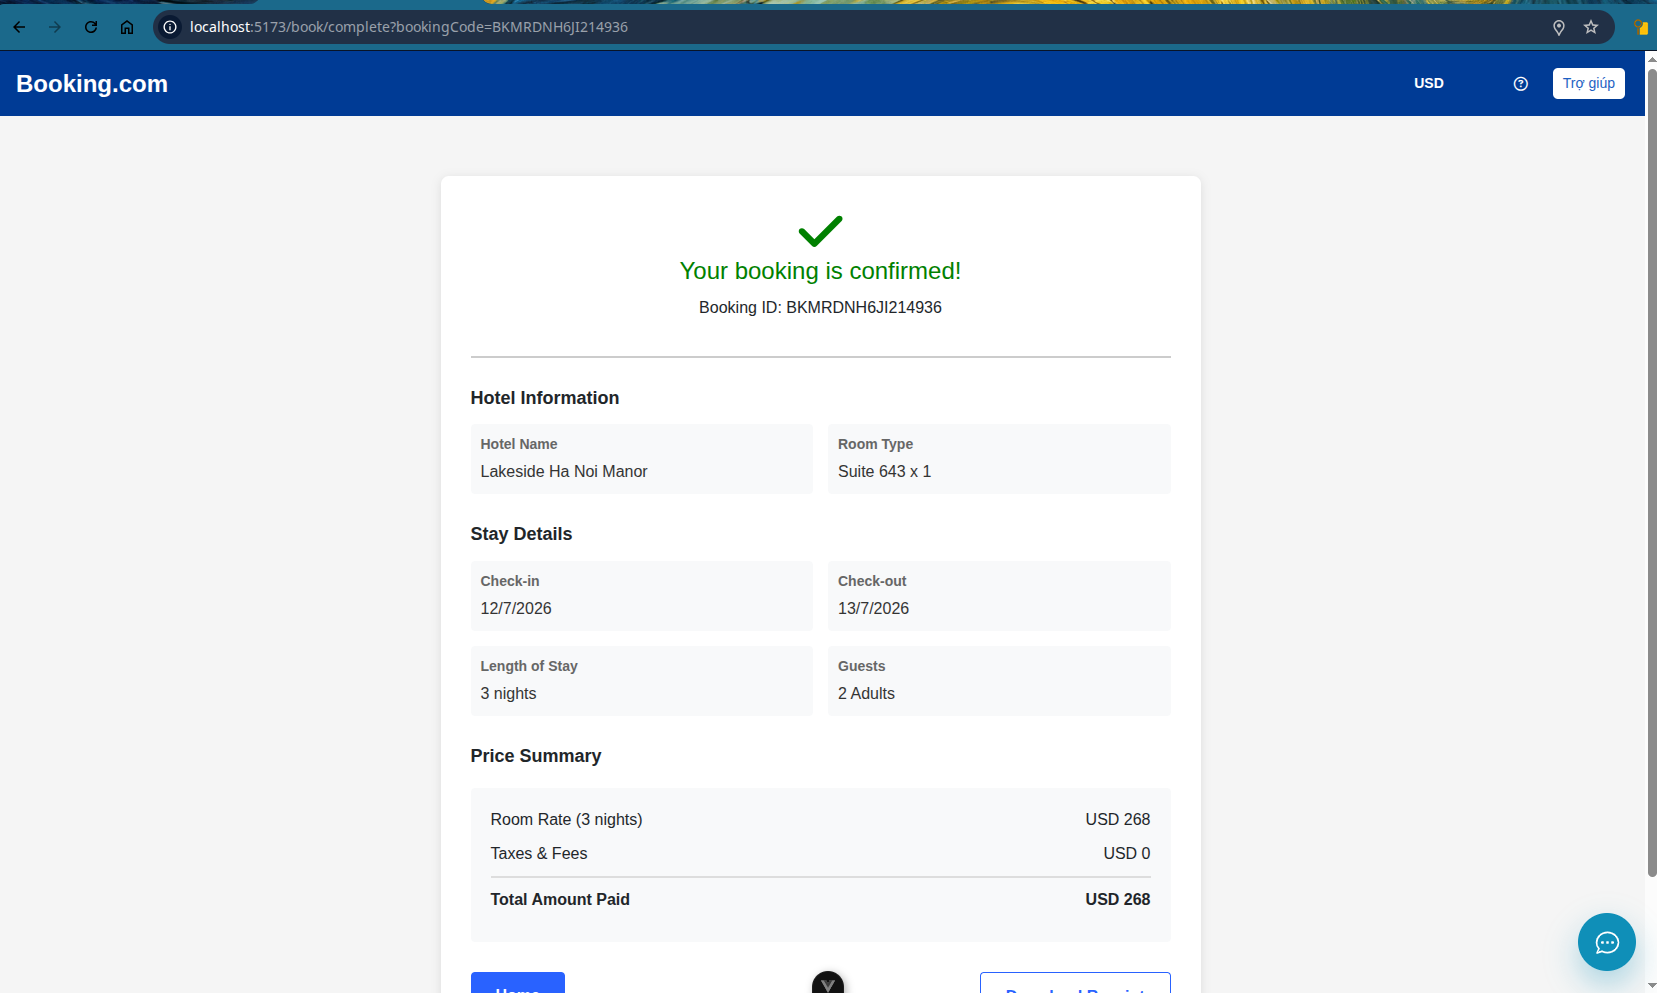
\includegraphics[width=0.95\textwidth]{images/ui_booking_success.png}
  \caption{Giao diện xác nhận đặt phòng thành công}
  \label{fig:ui_booking_success}
\end{figure}

Sau khi thanh toán thành công, hệ thống hiển thị modal xác nhận đặt phòng như Hình \ref{fig:ui_booking_success}, đồng thời gửi email xác nhận đến người dùng.

\begin{figure}[H]
  \centering
  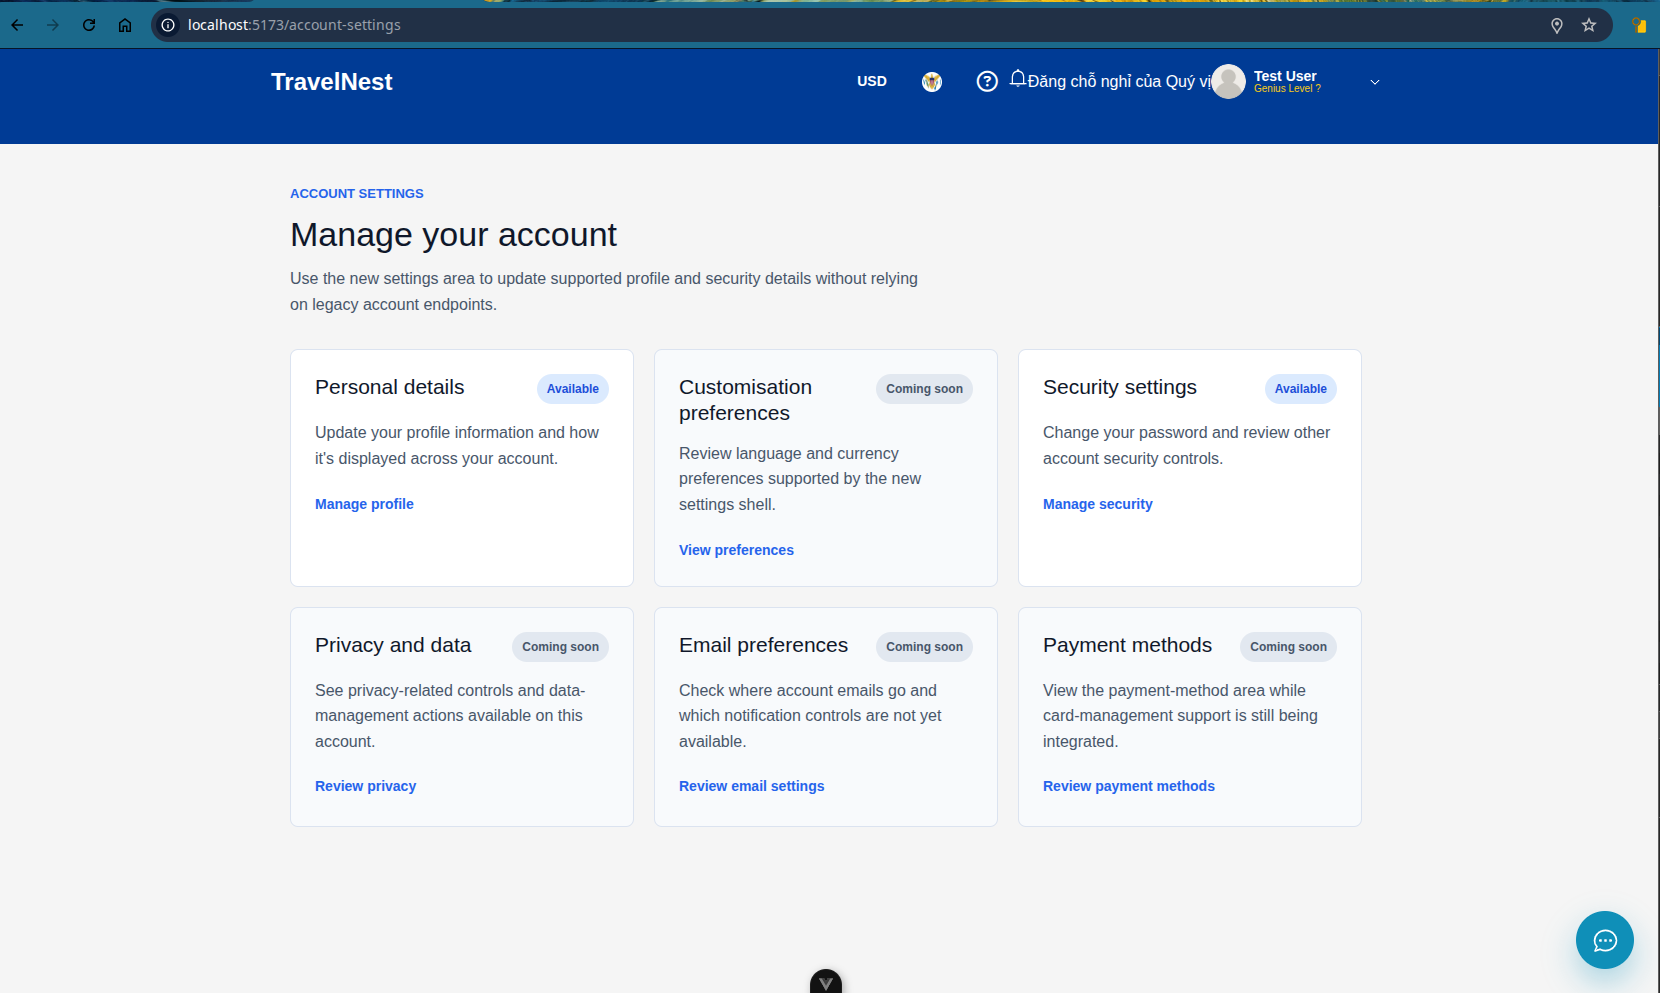
\includegraphics[width=0.95\textwidth]{images/ui_manage_account.png}
  \caption{Giao diện quản lý tài khoản người dùng}
  \label{fig:ui_account}
\end{figure}

Hình \ref{fig:ui_account} minh họa trang quản lý tài khoản, nơi người dùng có thể xem và cập nhật thông tin cá nhân, xem lịch sử đặt phòng và quản lý các đánh giá đã viết.

\subsubsection{Giao diện quản trị (Nuxt 4 Admin Dashboard)}

Bảng điều khiển quản trị được xây dựng bằng Nuxt 4 với Tailwind CSS và Element Plus, thiết kế theo dạng dashboard với sidebar navigation.

\begin{figure}[H]
  \centering
  % PLACEHOLDER: Giao diện admin dashboard
  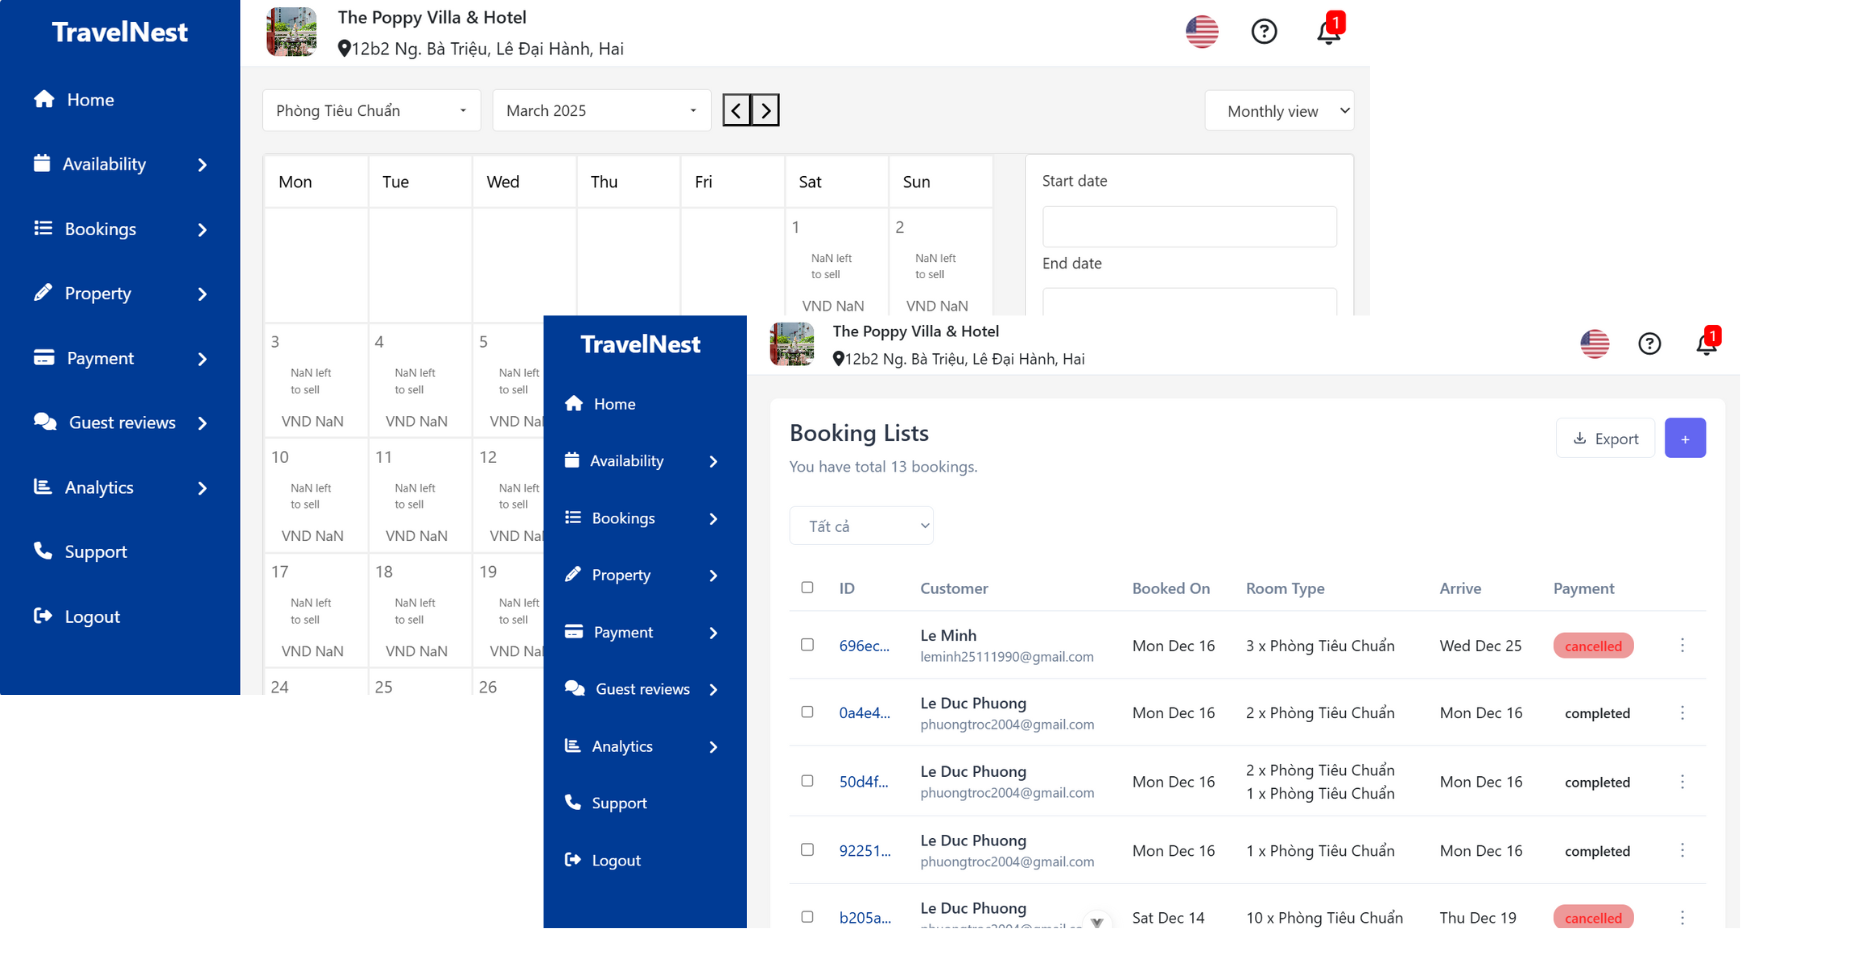
\includegraphics[width=0.95\textwidth]{images/ui_admin.png}
  \caption{Giao diện bảng điều khiển quản trị TravelNest (admin)}
  \label{fig:ui_admin}
\end{figure}

Hình \ref{fig:ui_admin} minh họa giao diện Admin Dashboard, bao gồm các khu vực chức năng:

\begin{itemize}
  \item \textbf{Tổng quan (Dashboard):} Biểu đồ doanh thu, số đơn đặt, tỷ lệ hủy, đánh giá trung bình.
  \item \textbf{Quản lý khách sạn:} Danh sách khách sạn, form thêm/sửa với các tab: thông tin chung, phòng, tiện nghi, chính sách, ảnh.
  \item \textbf{Quản lý đơn đặt:} Danh sách đơn đặt có thể lọc theo trạng thái, thời gian.
  \item \textbf{Quản lý đánh giá:} Đọc và phản hồi đánh giá từ khách hàng.
  \item \textbf{Báo cáo:} Báo cáo doanh thu chi tiết theo khách sạn, thời gian.
\end{itemize}

\subsection{Thiết kế lớp}

Phần này trình bày thiết kế chi tiết cho một số lớp quan trọng trong hệ thống.

\subsubsection{Lớp Booking và các lớp liên quan}

Hình \ref{fig:class_booking} mô tả biểu đồ lớp cho quy trình đặt phòng, thể hiện mối quan hệ giữa các lớp Booking, Hold, Room, RoomInventory, Payment, và các lớp liên quan.

\begin{figure}[H]
  \centering
  % PLACEHOLDER: Biểu đồ lớp Booking
  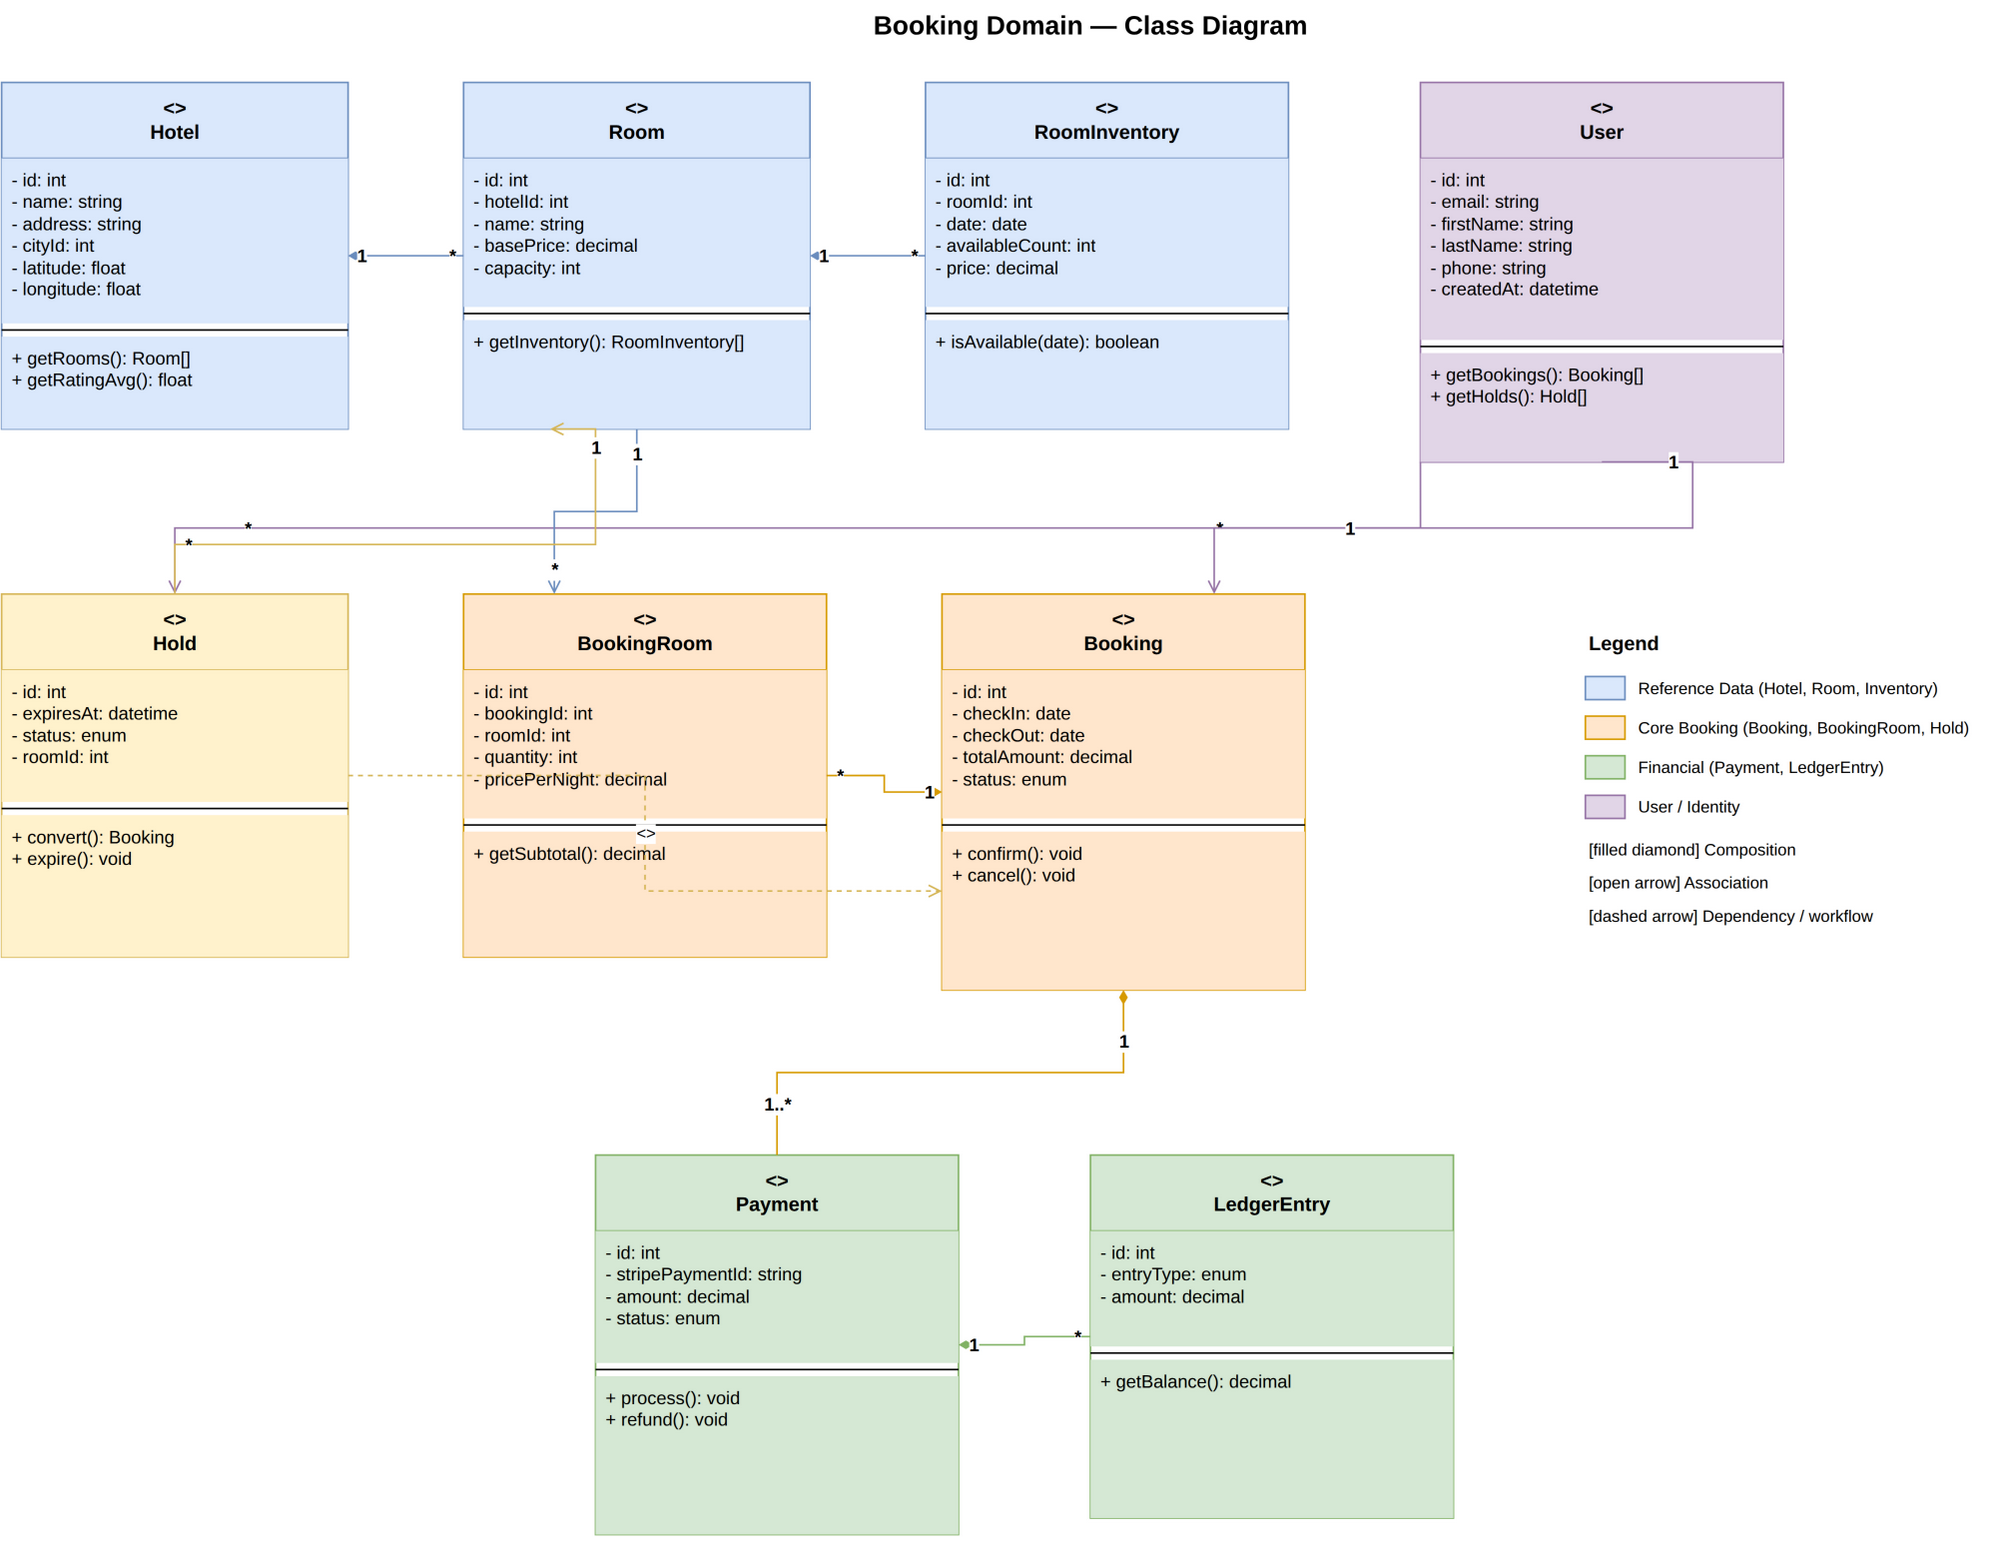
\includegraphics[width=0.95\textwidth]{images/fig_4_7_class_booking.png}
  \caption{Biểu đồ lớp cho quy trình đặt phòng}
  \label{fig:class_booking}
\end{figure}

Các quan hệ chính trong biểu đồ:

\begin{itemize}
  \item \textbf{Hotel} (1) ---- (N) \textbf{Room}: Một khách sạn có nhiều phòng.
  \item \textbf{Room} (1) ---- (N) \textbf{RoomInventory}: Mỗi phòng có danh sách tình trạng tồn kho theo ngày.
  \item \textbf{Booking} (N) ---- (N) \textbf{Room}: Một đơn đặt có thể bao gồm nhiều phòng (qua bảng trung gian BookingRoom).
  \item \textbf{Hold} (1) ---- (N) \textbf{HoldRoom}: Giữ chỗ tạm thời liên kết với các phòng được chọn.
  \item \textbf{Booking} (1) ----> (1) \textbf{Payment}: Mỗi đơn đặt có thể có một hoặc nhiều giao dịch thanh toán.
  \item \textbf{Payment} (1) ----> (0..1) \textbf{Refund}: Thanh toán có thể được hoàn tiền.
  \item \textbf{Payment} (1) ----> (N) \textbf{Transaction}: Lịch sử các bước xử lý thanh toán.
  \item \textbf{Payment} (1) ----> (N) \textbf{LedgerEntry}: Mỗi giao dịch tạo ra các bút toán trong sổ cái kép.
\end{itemize}

\subsubsection{Luồng truyền thông điệp --- Biểu đồ trình tự (Sequence Diagram)}

Hình \ref{fig:sequence_booking} mô tả biểu đồ trình tự cho use case "Đặt phòng", minh họa luồng truyền thông điệp giữa các đối tượng tham gia.

\begin{figure}[H]
  \centering
  % PLACEHOLDER: Biểu đồ trình tự đặt phòng
  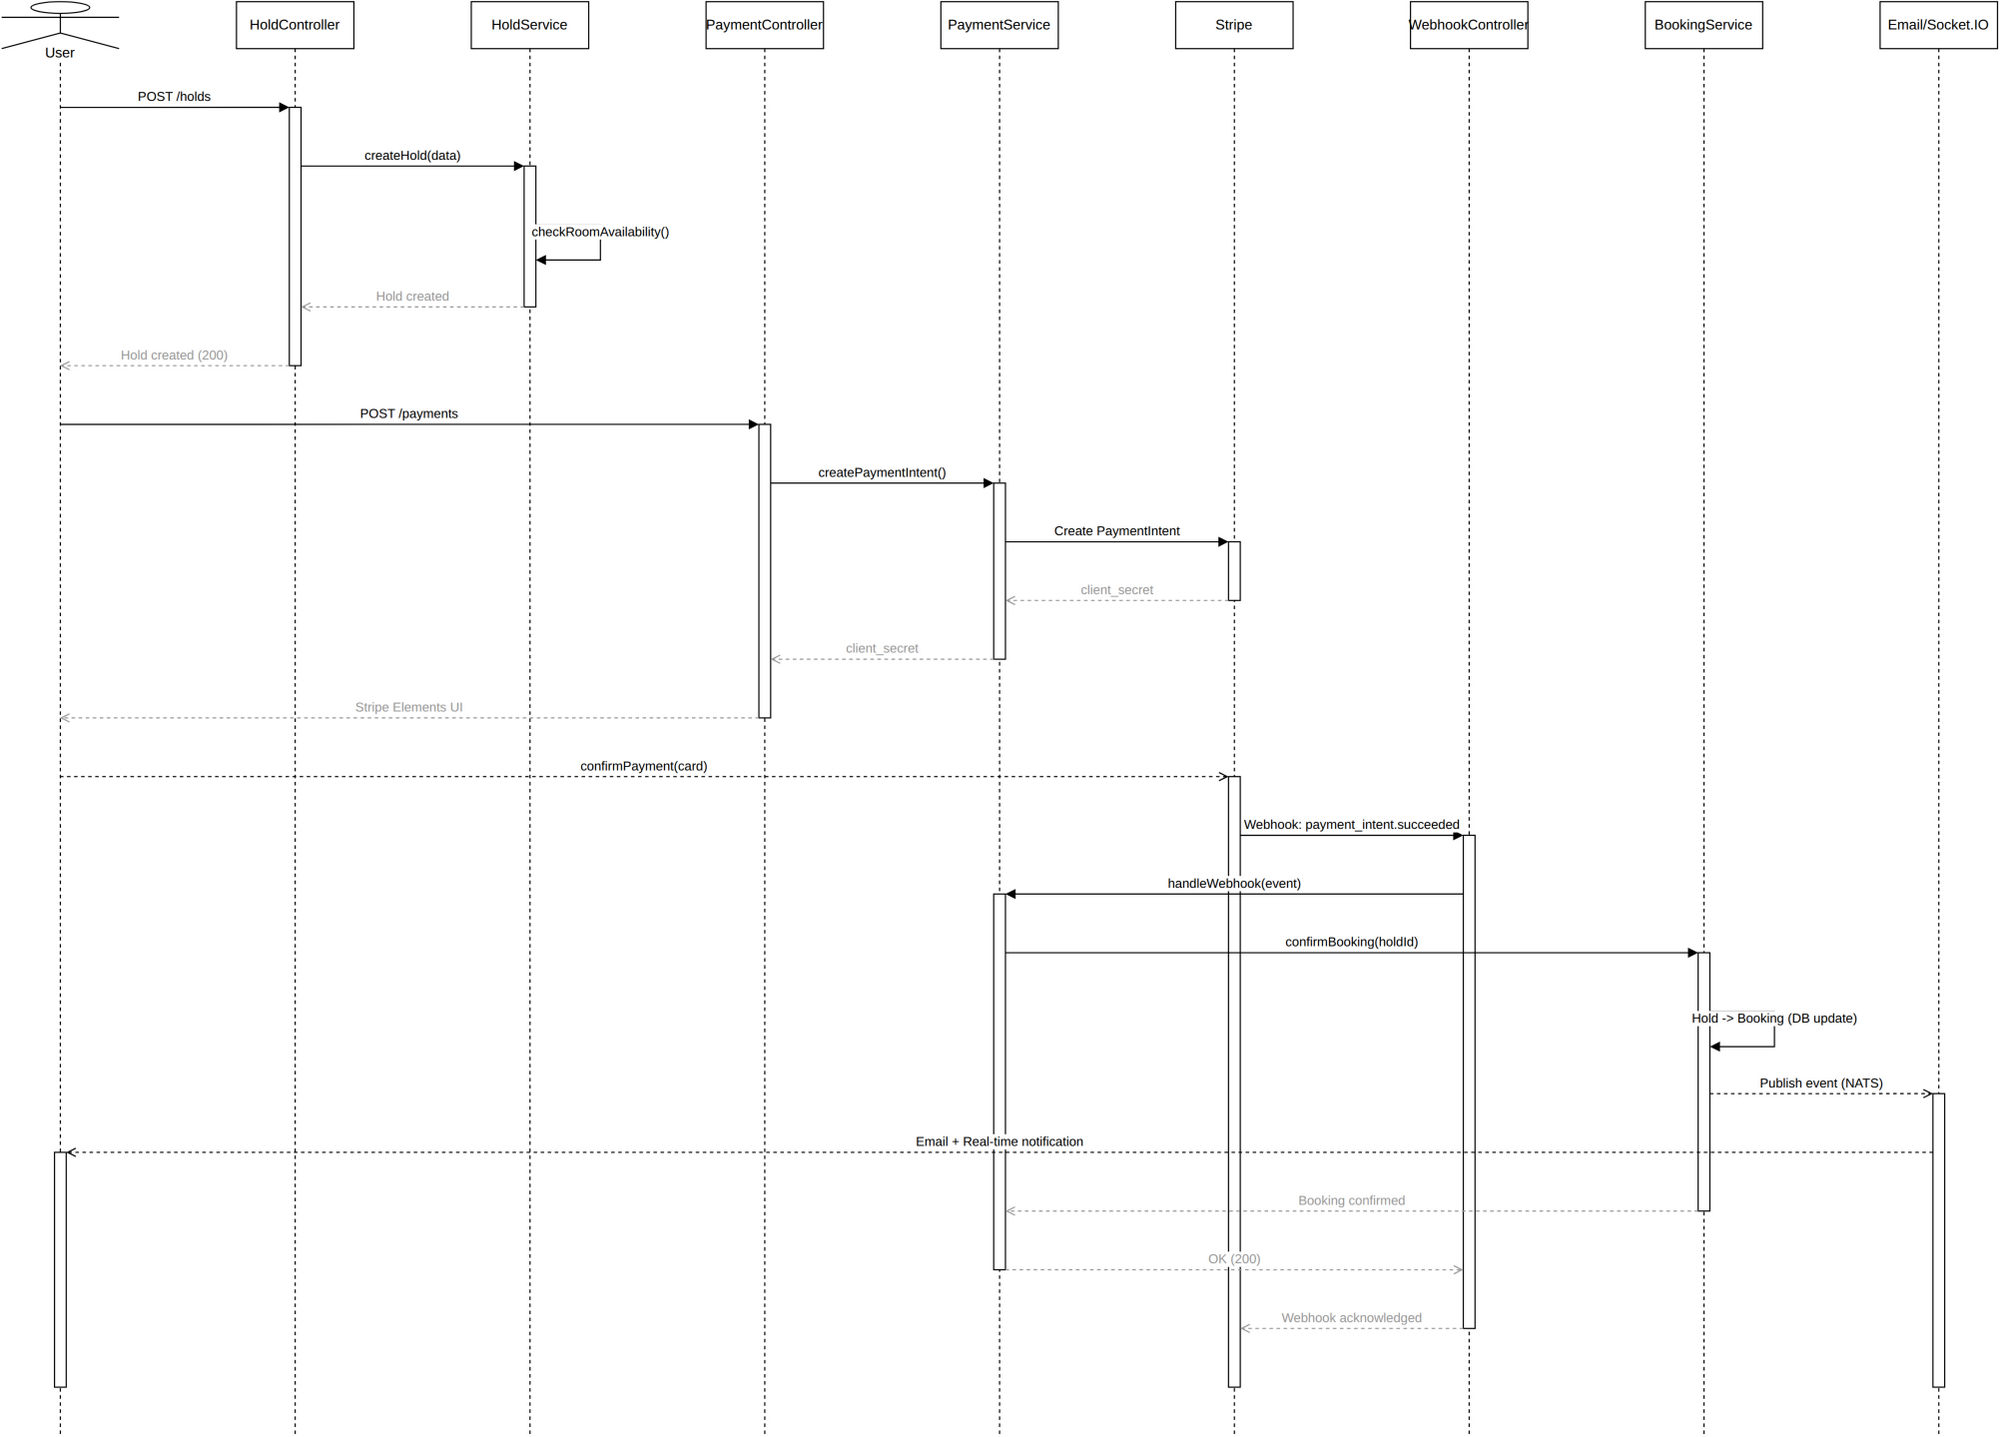
\includegraphics[width=0.95\textwidth]{images/fig_4_8_sequence_booking.png}
  \caption{Biểu đồ trình tự cho use case Đặt phòng}
  \label{fig:sequence_booking}
\end{figure}

Luồng truyền thông điệp cho đặt phòng diễn ra như sau:

\begin{enumerate}
  \item \texttt{User} gửi yêu cầu tạo Hold đến \texttt{HoldController}.
  \item \texttt{HoldController} gọi \texttt{HoldService.createHold()}.
  \item \texttt{HoldService} kiểm tra phòng trống qua \texttt{RoomInventoryRepository}, tạo \texttt{Hold} và \texttt{HoldRoom}.
  \item \texttt{HoldService} gọi \texttt{HoldExpiryQueue.add()} với delay 15 phút.
  \item \texttt{User} gửi yêu cầu thanh toán đến \texttt{PaymentController}.
  \item \texttt{PaymentController} gọi \texttt{PaymentService.createPaymentIntent()}.
  \item \texttt{PaymentService} tạo \texttt{IdempotencyKey}, gọi Stripe API tạo PaymentIntent.
  \item \texttt{User} xác nhận thanh toán trên Stripe, Stripe gửi webhook đến \texttt{WebhookController}.
  \item \texttt{WebhookController} gọi \texttt{PaymentService.handleWebhook()}.
  \item \texttt{PaymentService} xác minh webhook, gọi \texttt{BookingService.confirmBooking()}.
  \item \texttt{BookingService} chuyển \texttt{Hold} thành \texttt{Booking}, cập nhật \texttt{RoomInventory}.
  \item \texttt{BookingService} gọi \texttt{LedgerService.createEntries()} để ghi sổ kép.
  \item \texttt{BookingService} gọi \texttt{EmailEvent.publish()} lên NATS để gửi email xác nhận.
  \item \texttt{BookingService} gọi \texttt{SocketService.emit()} để gửi thông báo real-time đến chủ khách sạn.
\end{enumerate}

\subsection{Thiết kế cơ sở dữ liệu}

\subsubsection{Biểu đồ thực thể liên kết (ERD)}

Hình \ref{fig:erd} trình bày biểu đồ thực thể liên kết (Entity-Relationship Diagram) cho cơ sở dữ liệu MySQL của hệ thống TravelNest.

\begin{figure}[H]
  \centering
  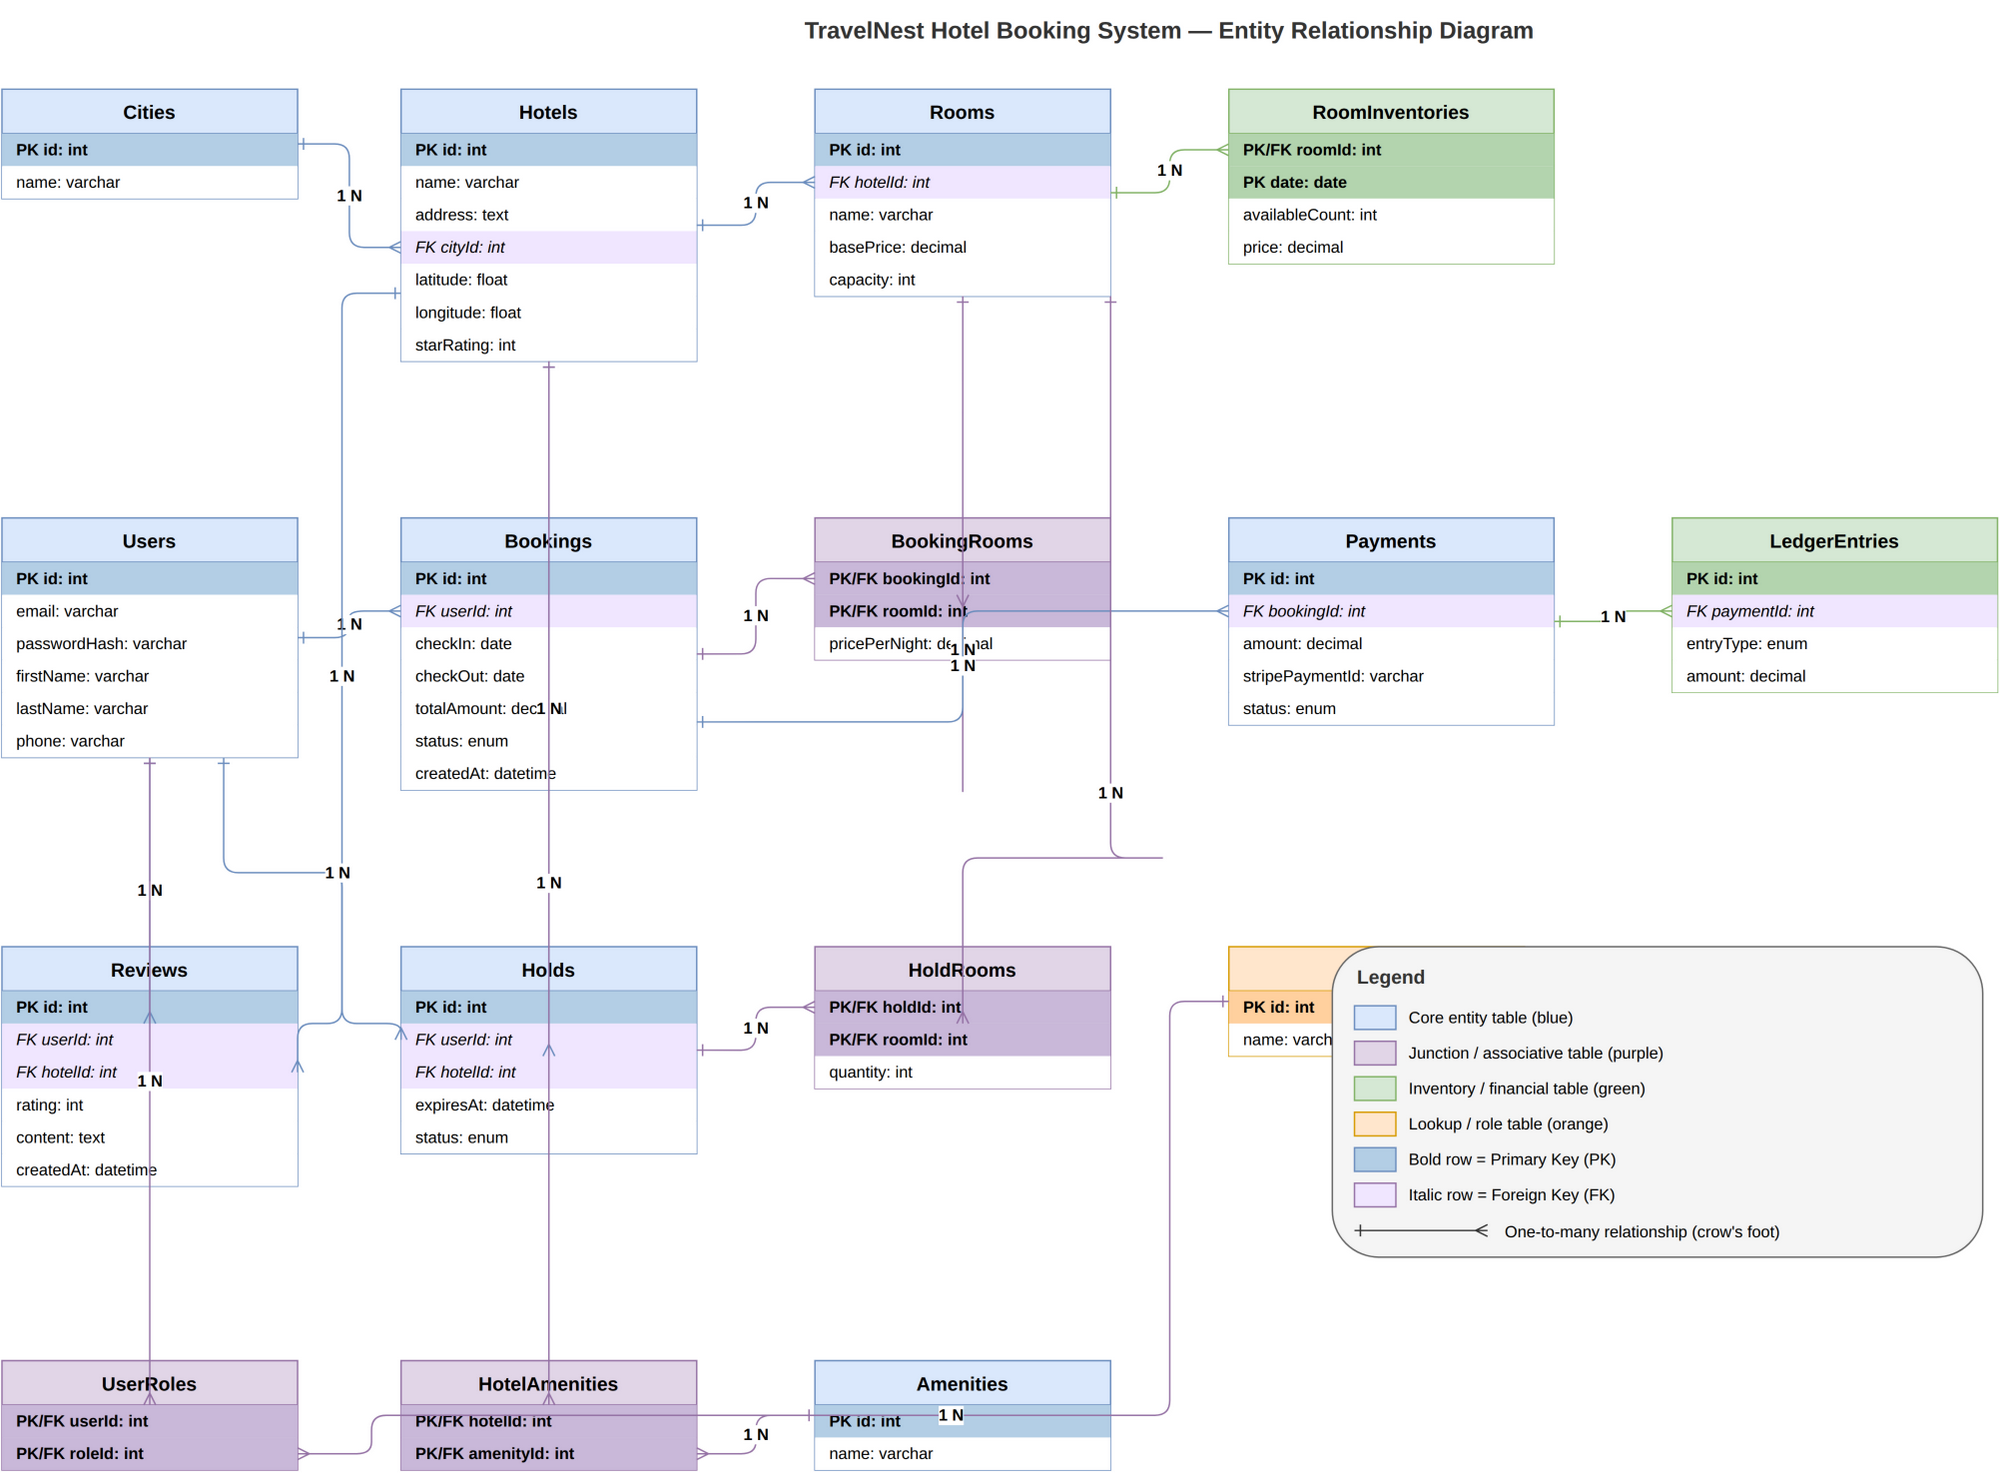
\includegraphics[width=0.95\textwidth]{images/fig_4_9_erd.png}
  \caption{Biểu đồ thực thể liên kết (ERD) của hệ thống TravelNest}
  \label{fig:erd}
\end{figure}

Cơ sở dữ liệu MySQL của TravelNest bao gồm 47 bảng, được tổ chức thành các nhóm chính sau:

\begin{enumerate}
  \item \textbf{Nhóm Người dùng và Xác thực (User \& Auth):}
  \begin{itemize}
    \item \texttt{Users}: Thông tin người dùng (email, password hash, tên, số điện thoại, avatar).
    \item \texttt{AuthAccounts}: Liên kết OAuth (provider, providerId).
    \item \texttt{Roles}, \texttt{UserRoles}: Phân quyền theo vai trò.
    \item \texttt{Permissions}, \texttt{RolePermissions}: Quyền chi tiết cho từng vai trò.
  \end{itemize}

  \item \textbf{Nhóm Khách sạn và Phòng (Hotel \& Room):}
  \begin{itemize}
    \item \texttt{Hotels}: Thông tin khách sạn (tên, mô tả, địa chỉ, tọa độ).
    \item \texttt{Rooms}: Các loại phòng trong khách sạn (tên, mô tả, sức chứa, giá gốc).
    \item \texttt{RoomInventories}: Tình trạng phòng trống theo ngày (date, availableCount, price).
    \item \texttt{HotelAmenities}, \texttt{RoomAmenities}: Tiện nghi của khách sạn và phòng.
    \item \texttt{HotelPolicies}, \texttt{HotelCancellationRules}: Chính sách và quy định hủy phòng.
    \item \texttt{Images}, \texttt{ImageVariants}: Ảnh khách sạn (gốc và các kích thước đã resize).
  \end{itemize}

  \item \textbf{Nhóm Đặt phòng (Booking):}
  \begin{itemize}
    \item \texttt{Bookings}: Đơn đặt phòng (ngày nhận, ngày trả, trạng thái, tổng tiền).
    \item \texttt{BookingRooms}: Quan hệ N-N giữa Booking và Room.
    \item \texttt{Holds}: Giữ chỗ tạm thời (thời gian hết hạn).
    \item \texttt{HoldRooms}: Phòng được giữ trong một Hold.
  \end{itemize}

  \item \textbf{Nhóm Thanh toán (Payment):}
  \begin{itemize}
    \item \texttt{Payments}: Giao dịch thanh toán (số tiền, trạng thái, Stripe PaymentIntent ID).
    \item \texttt{Refunds}: Giao dịch hoàn tiền.
    \item \texttt{Payouts}, \texttt{PayoutItems}: Chi trả cho chủ khách sạn.
    \item \texttt{Transactions}: Nhật ký các bước xử lý thanh toán.
    \item \texttt{LedgerAccounts}, \texttt{LedgerEntries}: Sổ cái kép (double-entry ledger).
    \item \texttt{Invoices}: Hóa đơn điện tử.
    \item \texttt{IdempotencyKeys}: Khóa chống trùng lặp thanh toán.
    \item \texttt{ConnectedPaymentAccounts}: Tài khoản Stripe Connect của chủ khách sạn.
    \item \texttt{WebhookEventLogs}: Nhật ký webhook từ Stripe.
  \end{itemize}

  \item \textbf{Nhóm Đánh giá (Review):}
  \begin{itemize}
    \item \texttt{Reviews}: Đánh giá của khách hàng (điểm số, nội dung).
    \item \texttt{ReviewMedia}: Ảnh/video đính kèm đánh giá.
    \item \texttt{ReviewReplies}: Phản hồi của chủ khách sạn.
    \item \texttt{ReviewHelpfulVotes}: Bình chọn "Hữu ích" cho đánh giá.
    \item \texttt{HotelRatingSummaries}: Điểm đánh giá trung bình của khách sạn (cache).
  \end{itemize}

  \item \textbf{Nhóm Địa lý (Geography):}
  \begin{itemize}
    \item \texttt{Countries}, \texttt{Cities}, \texttt{Destinations}: Dữ liệu địa lý.
    \item \texttt{NearByPlaces}: Địa điểm du lịch gần khách sạn.
  \end{itemize}

  \item \textbf{Nhóm Khác:}
  \begin{itemize}
    \item \texttt{Notifications}: Thông báo cho người dùng.
    \item \texttt{HotelSearchSnapshots}: Snapshot khách sạn dùng để sync sang Elasticsearch.
    \item \texttt{SavedHotels}: Khách sạn yêu thích.
    \item \texttt{ViewedHotels}: Lịch sử xem khách sạn.
    \item \texttt{HotelUsers}: Phân quyền quản lý khách sạn cho người dùng.
  \end{itemize}
\end{enumerate}

\subsubsection{Chiến lược đánh chỉ mục (Indexing)}

Để đảm bảo hiệu năng truy vấn, các chỉ mục (index) được tạo trên các cột thường xuyên được sử dụng trong điều kiện WHERE và JOIN:

\begin{itemize}
  \item \texttt{RoomInventories}: Composite index trên (roomId, date) để kiểm tra nhanh tình trạng phòng trống theo ngày.
  \item \texttt{Bookings}: Index trên (userId, status) và (hotelId, checkInDate) để truy vấn đơn đặt theo người dùng và khách sạn.
  \item \texttt{Hotels}: Index trên (cityId, countryId) để lọc khách sạn theo địa điểm.
  \item \texttt{Reviews}: Index trên (hotelId, createdAt) để phân trang đánh giá.
  \item \texttt{Holds}: Index trên (expiresAt) để worker có thể quét nhanh các hold đã hết hạn.
\end{itemize}

\section{Xây dựng ứng dụng}

\subsection{Thư viện và công cụ sử dụng}

Bảng \ref{tab:tools} liệt kê các công cụ, ngôn ngữ lập trình, thư viện và môi trường phát triển đã sử dụng trong quá trình xây dựng TravelNest.

\begin{table}[H]
  \centering
  \caption{Danh sách thư viện và công cụ sử dụng}
  \label{tab:tools}
  \begin{tabularx}{\textwidth}{p{4cm} p{3cm} X}
    \toprule
    \textbf{Mục đích} & \textbf{Công cụ / Phiên bản} & \textbf{Ghi chú} \\
    \midrule
    IDE & VS Code & Môi trường phát triển chính \\
    Node.js Runtime & Node.js 18+ & Backend JavaScript runtime \\
    Package Manager & Yarn 1.22+ & Monorepo với Yarn Workspaces \\
    Go Runtime & Go 1.22 & Microservices \\
    Database GUI & MySQL Workbench, MongoDB Compass & Quản lý cơ sở dữ liệu \\
    API Testing & Postman, Swagger UI & Kiểm thử API \\
    Containerization & Docker 24+ & Đóng gói ứng dụng \\
    Container Orchestration & Kubernetes (k3s) 1.28+ & Triển khai production \\
    GitOps & Argo CD & Đồng bộ deployment tự động \\
    CI/CD & GitHub Actions & Tự động hóa build \& deploy \\
    Tunnel & Cloudflare Tunnel & Public ingress không cần public IP \\
    Monitoring & Kibana & Xem log từ Elasticsearch \\
    Linting (JS) & ESLint, Prettier & Chuẩn hóa mã nguồn \\
    Linting (Go) & golangci-lint & Chuẩn hóa mã nguồn Go \\
    Testing (Node.js) & Jest & Unit test và integration test \\
    \bottomrule
  \end{tabularx}
\end{table}

\subsection{Kết quả đạt được}

Sau quá trình phát triển, hệ thống TravelNest đã đạt được những kết quả cụ thể như trình bày trong Bảng \ref{tab:dev_stats}:

\begin{table}[H]
  \centering
  \caption{Thống kê kết quả phát triển}
  \label{tab:dev_stats}
  \begin{tabularx}{\textwidth}{p{6cm} X}
    \toprule
    \textbf{Chỉ số} & \textbf{Giá trị} \\
    \midrule
    Tổng số bảng MySQL & 47 bảng \\
    Số nhóm API (route groups) & 15 nhóm \\
    Số endpoint API & 80+ endpoints \\
    Số model Sequelize & 47 models \\
    Số service (Node.js) & 24 services \\
    Số repository & 22 repositories \\
    Số Go microservice & 3 services \\
    Số Docker image & 7 images \\
    Số GitHub Actions workflow & 6 workflows \\
    Hỗ trợ ngôn ngữ & 2 (Tiếng Việt, Tiếng Anh) \\
    Số worker BullMQ & 3 workers \\
    Phương thức xác thực & 3 (Email/Password, Google OAuth, Twitter OAuth) \\
    Cổng thanh toán & 1 (Stripe) \\
    Kênh thông báo & 3 (Email, SMS, Real-time) \\
    \bottomrule
  \end{tabularx}
\end{table}

\subsection{Minh họa các chức năng chính}

Phần này trình bày một số màn hình minh họa cho các chức năng chính của hệ thống.

\begin{figure}[H]
  \centering
  % PLACEHOLDER: Trang tìm kiếm
  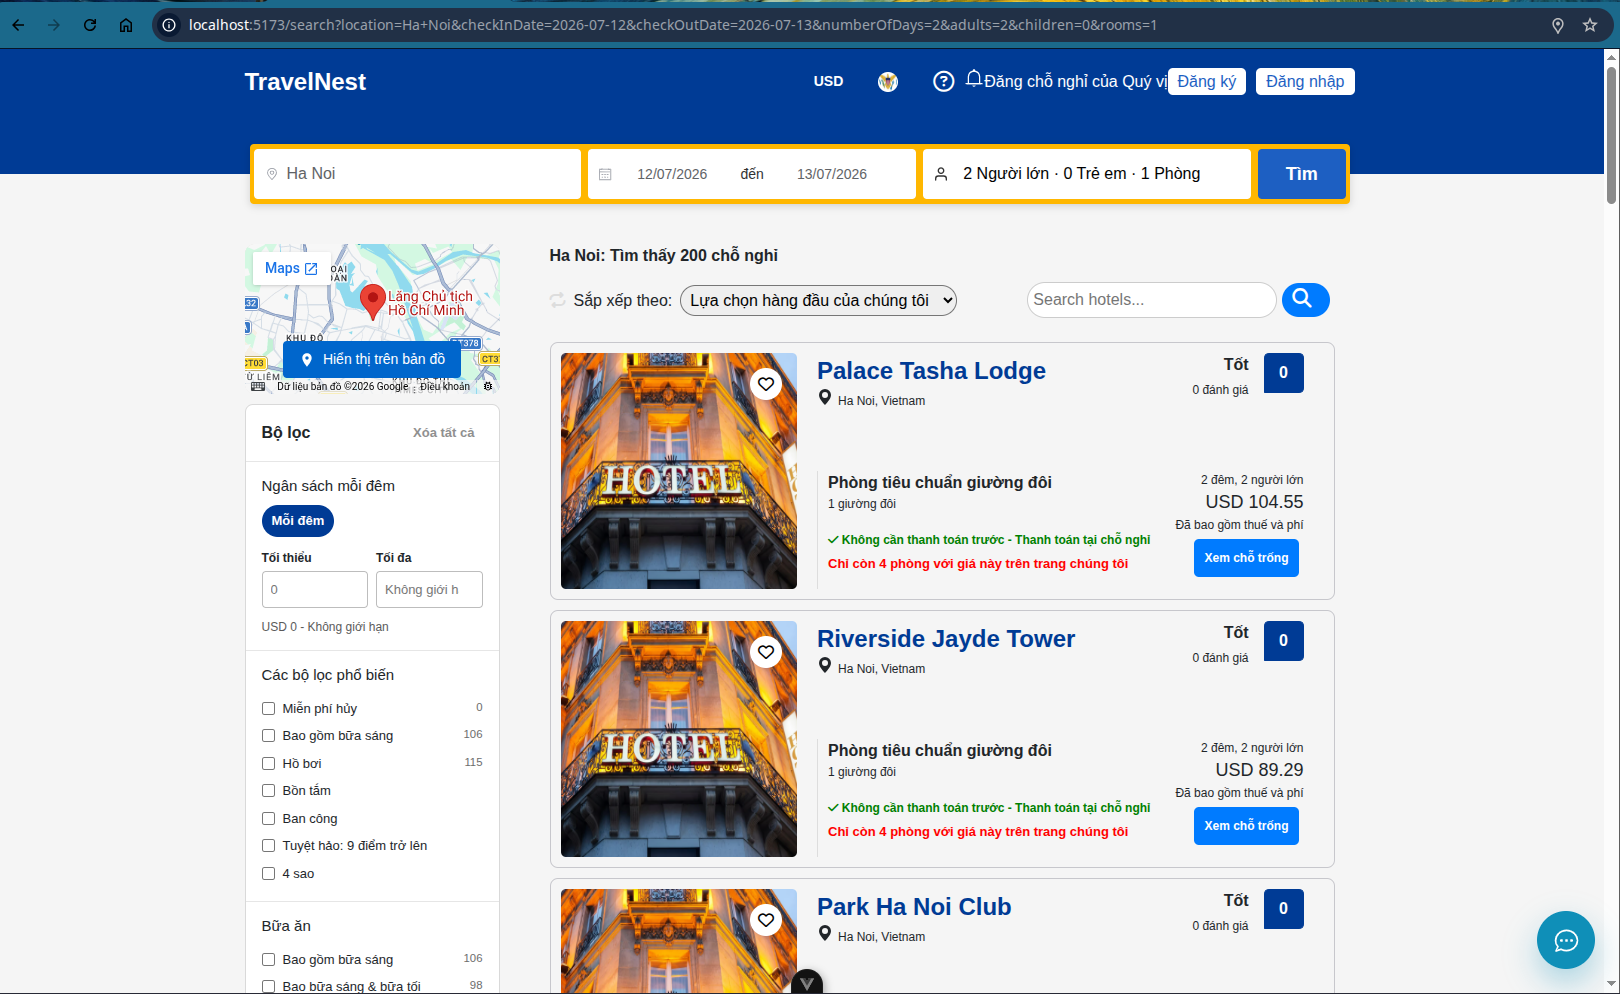
\includegraphics[width=0.95\textwidth]{images/ui_search_results.png}
  \caption{Màn hình kết quả tìm kiếm khách sạn}
  \label{fig:ui_search}
\end{figure}

Hình \ref{fig:ui_search} hiển thị trang kết quả tìm kiếm, nơi người dùng có thể xem danh sách khách sạn dưới dạng card, lọc kết quả theo giá và đánh giá, và xem vị trí trên bản đồ Leaflet.

\begin{figure}[H]
  \centering
  % PLACEHOLDER: Trang thanh toán
  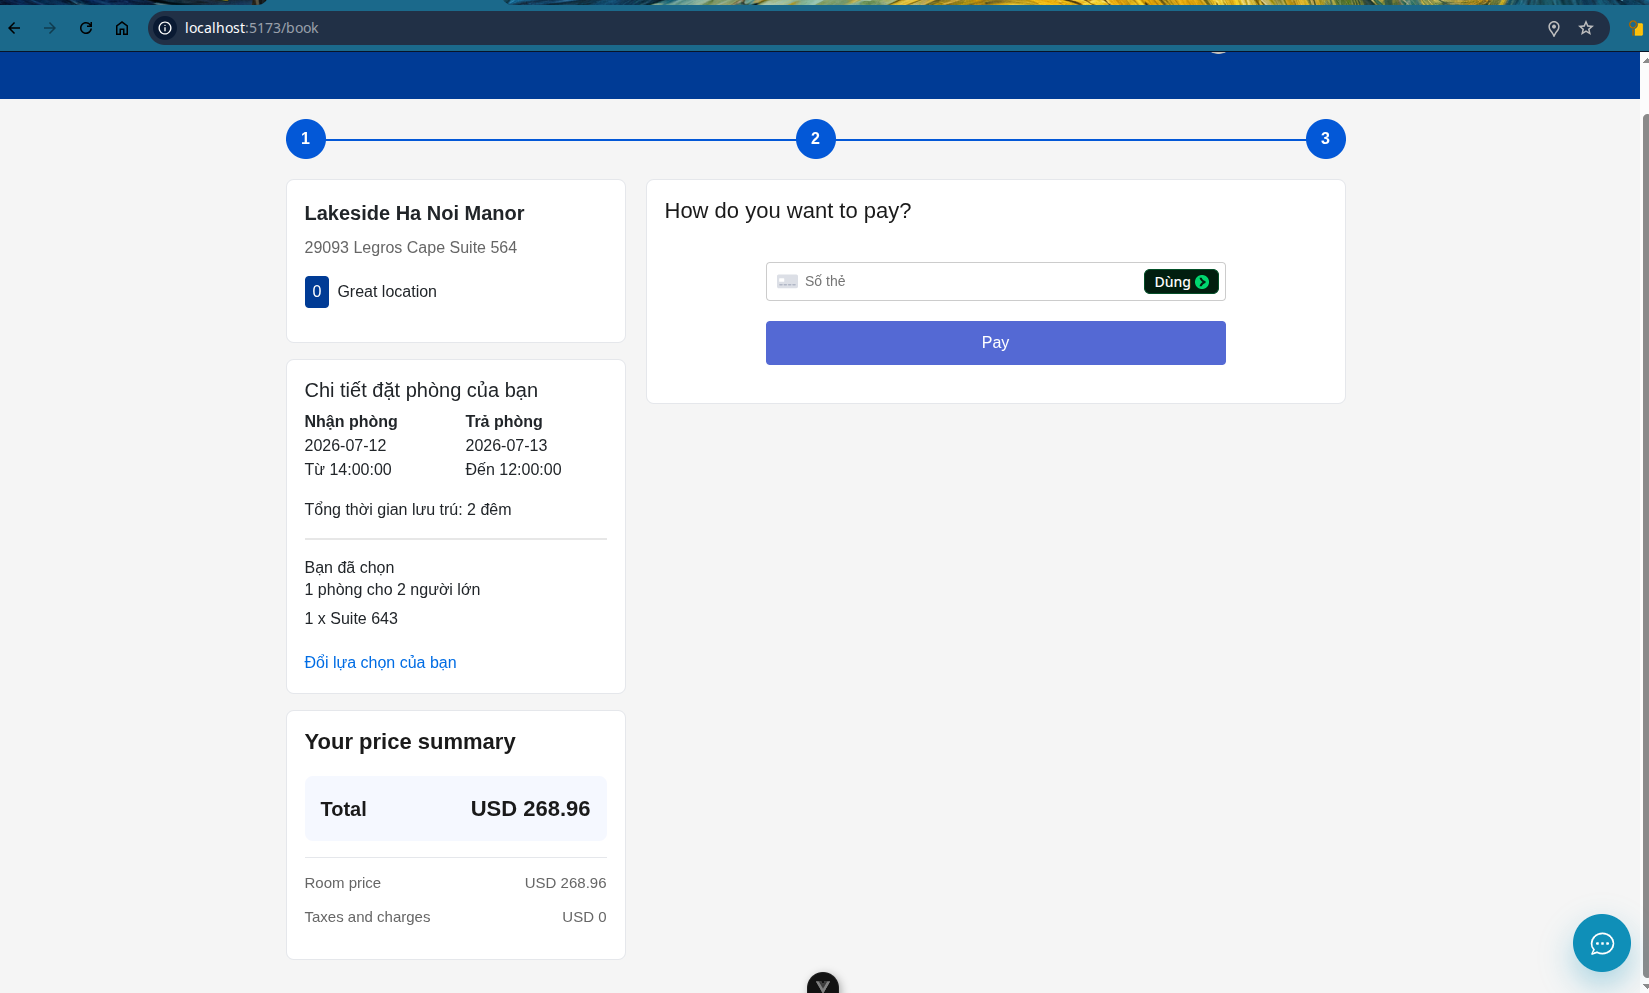
\includegraphics[width=0.95\textwidth]{images/ui_checkout_payment.png}
  \caption{Màn hình thanh toán với Stripe}
  \label{fig:ui_payment}
\end{figure}

Hình \ref{fig:ui_payment} minh họa màn hình thanh toán, nơi người dùng xem tóm tắt đơn đặt và nhập thông tin thẻ qua Stripe Elements.

\section{Kiểm thử}

Hệ thống TravelNest được kiểm thử ở nhiều cấp độ khác nhau để đảm bảo chất lượng.

\subsection{Kiểm thử đơn vị (Unit Testing)}

Unit test được thực hiện cho các service và repository trong backend Node.js sử dụng Jest framework. Các test tập trung vào:

\begin{itemize}
  \item Các hàm xử lý logic nghiệp vụ trong Services (ví dụ: tính tổng tiền đặt phòng, kiểm tra tính hợp lệ của ngày).
  \item Các hàm truy vấn cơ sở dữ liệu trong Repositories (sử dụng mock Sequelize models).
  \item Các hàm validation trong Validators (sử dụng Joi schemas).
  \item Các hàm xử lý trong Go microservices (sử dụng Go testing package).
\end{itemize}

\subsection{Kiểm thử tích hợp (Integration Testing)}

Integration test kiểm tra sự tương tác giữa các thành phần:

\begin{itemize}
  \item Kiểm thử luồng đặt phòng hoàn chỉnh: từ tạo Hold -> thanh toán -> xác nhận Booking.
  \item Kiểm thử webhook Stripe: mô phỏng webhook để đảm bảo hệ thống xử lý đúng các sự kiện từ Stripe.
  \item Kiểm thử giao tiếp NATS: đảm bảo event được publish và consume đúng cách.
  \item Kiểm thử đồng bộ Elasticsearch: đảm bảo dữ liệu khách sạn được index chính xác.
\end{itemize}

\subsection{Trường hợp kiểm thử cho chức năng đặt phòng}

Bảng \ref{tab:test_booking} trình bày một số trường hợp kiểm thử quan trọng cho chức năng đặt phòng.

\begin{table}[H]
  \centering
  \caption{Trường hợp kiểm thử cho chức năng đặt phòng}
  \label{tab:test_booking}
  \begin{tabularx}{\textwidth}{p{1cm} p{3cm} X X}
    \toprule
    \textbf{STT} & \textbf{Mô tả} & \textbf{Dữ liệu đầu vào} & \textbf{Kết quả mong đợi} \\
    \midrule
    TC-01 & Đặt phòng thành công & User đã đăng nhập, phòng trống, thẻ hợp lệ & Booking được tạo với trạng thái Confirmed, email xác nhận được gửi \\
    TC-02 & Đặt phòng khi phòng đã hết & Không còn phòng trống trong ngày đã chọn & Hệ thống trả về lỗi "Phòng không khả dụng" \\
    TC-03 & Thanh toán thất bại (thẻ không hợp lệ) & Số thẻ không hợp lệ & Hệ thống trả về lỗi từ Stripe, Hold vẫn được giữ đến khi hết hạn \\
    TC-04 & Hold hết hạn trước khi thanh toán & Không thanh toán trong 15 phút & Worker tự động hủy Hold và giải phóng phòng \\
    TC-05 & Đặt phòng trùng lặp (idempotency) & Gửi 2 lần cùng idempotency key & Chỉ tạo 1 Booking, request thứ 2 trả về Booking đã tồn tại \\
    TC-06 & Hủy đặt phòng thành công & Booking đã Confirmed, trong thời hạn hủy miễn phí & Booking chuyển sang Cancelled, hoàn tiền được xử lý \\
    \bottomrule
  \end{tabularx}
\end{table}

\subsection{Kết quả kiểm thử}

Tổng cộng đã thiết kế và thực hiện hơn 50 trường hợp kiểm thử cho các chức năng chính của hệ thống. Kết quả cho thấy tất cả các trường hợp kiểm thử quan trọng đều đạt (pass), đặc biệt là các luồng liên quan đến đặt phòng và thanh toán --- những chức năng nhạy cảm nhất về mặt dữ liệu. Một số lỗi nhỏ liên quan đến validation dữ liệu đầu vào đã được phát hiện và sửa chữa trong quá trình kiểm thử.

\section{Triển khai}

\subsection{Mô hình triển khai}

Hệ thống TravelNest được triển khai trên một cụm Kubernetes (k3s) chạy trên VPS (Virtual Private Server), sử dụng Cloudflare Tunnel để public ra internet mà không cần mở port trực tiếp.

\begin{figure}[H]
  \centering
  % PLACEHOLDER: Sơ đồ triển khai
  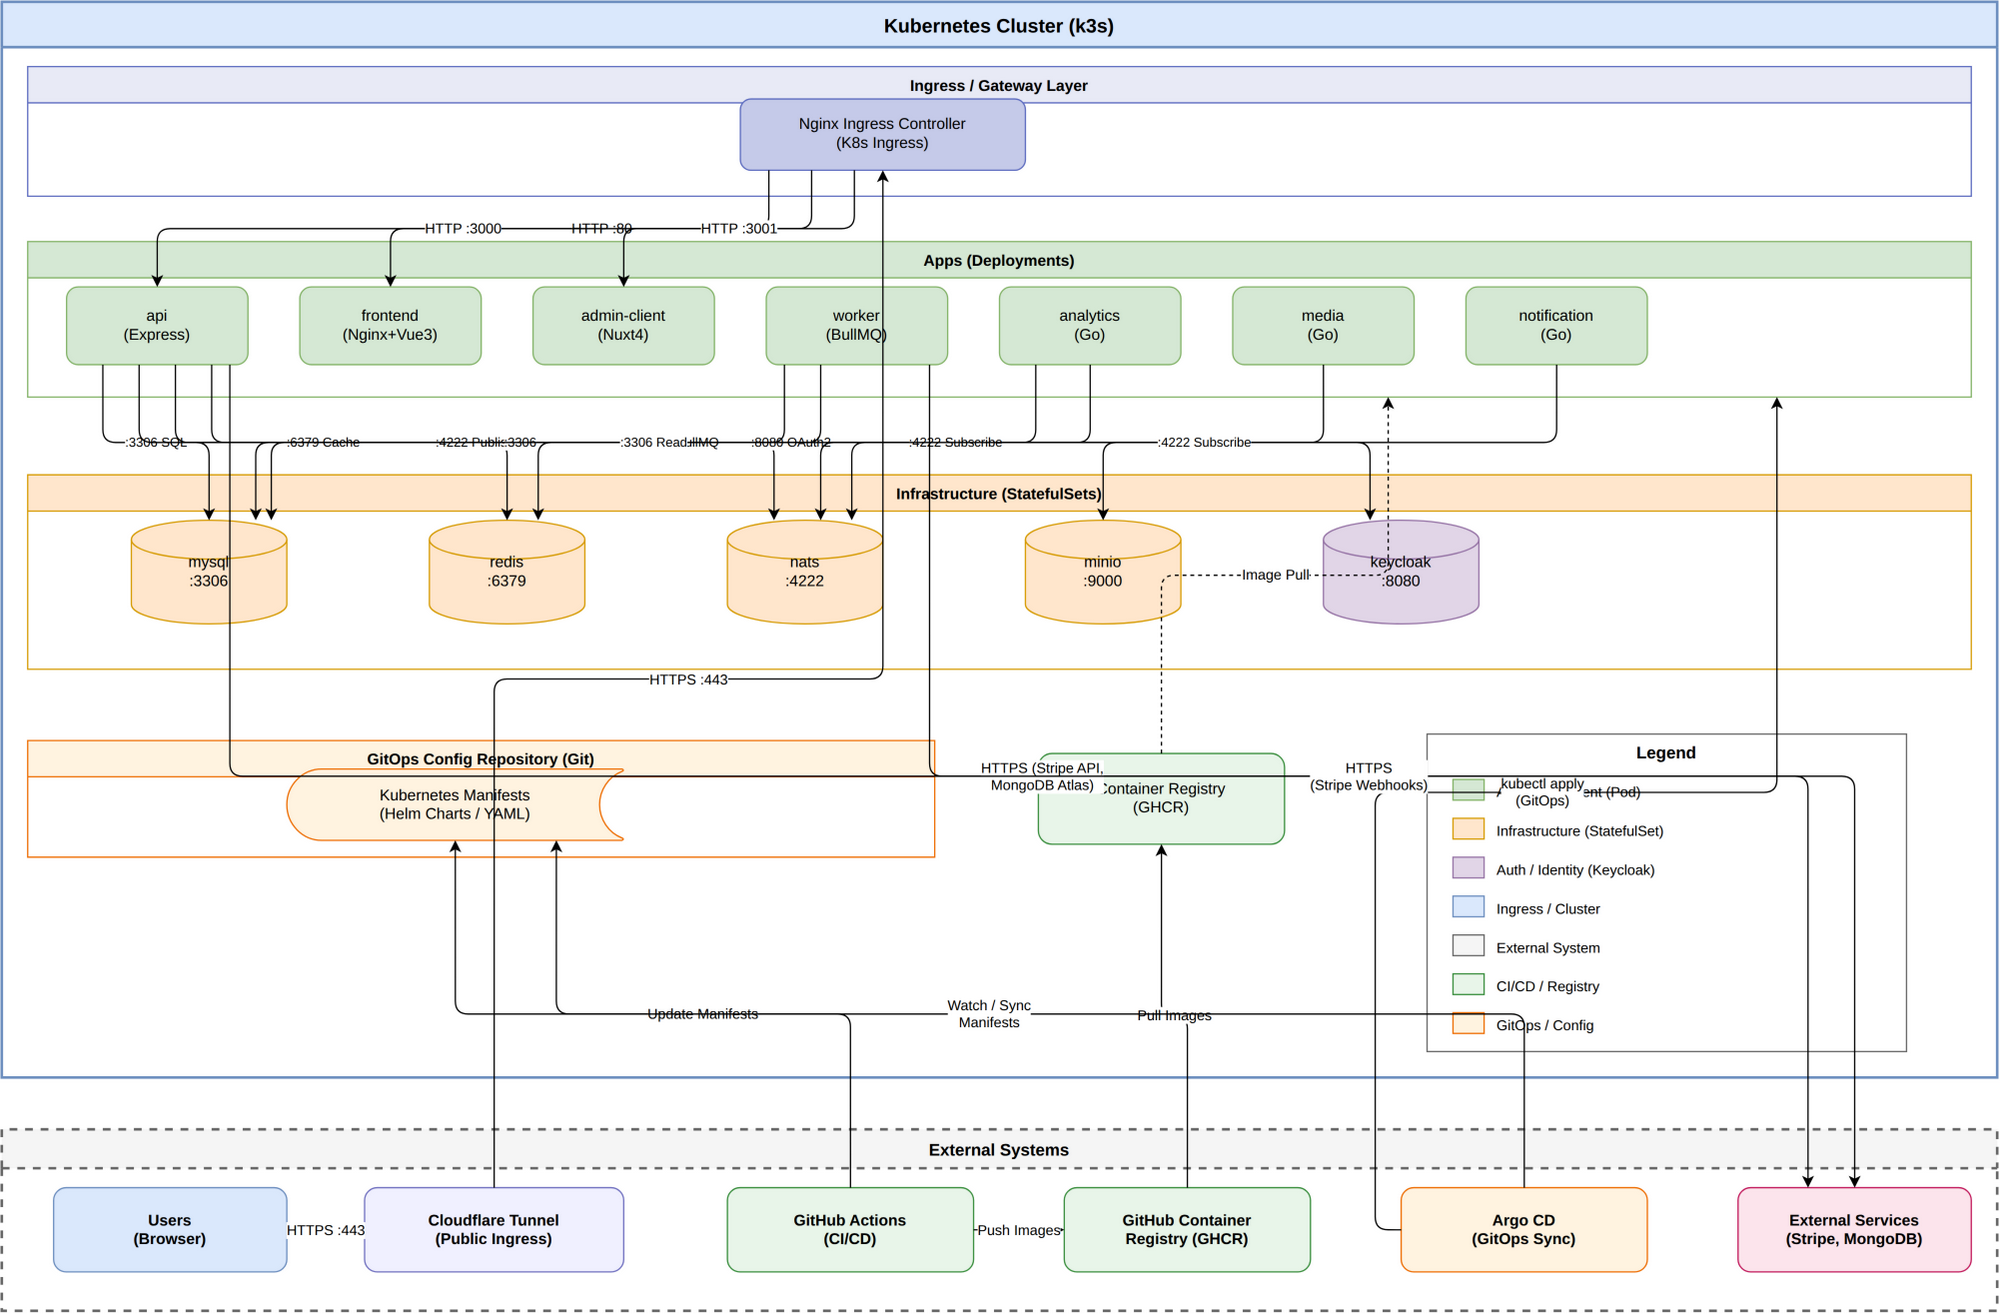
\includegraphics[width=0.95\textwidth]{images/fig_4_12_deployment.png}
  \caption{Sơ đồ triển khai hệ thống TravelNest trên Kubernetes}
  \label{fig:deployment}
\end{figure}

Như minh họa ở Hình \ref{fig:deployment}, cụm Kubernetes bao gồm các thành phần sau, được quản lý bởi Argo CD:

\begin{itemize}
  \item \textbf{7 ứng dụng (Deployments):}
  \begin{enumerate}
    \item \texttt{api} --- Node.js Express API server (port 3000).
    \item \texttt{frontend} --- Vue 3 SPA, phục vụ bởi Nginx (port 80).
    \item \texttt{admin-client} --- Nuxt 4 Admin Dashboard (port 8000).
    \item \texttt{worker} --- BullMQ worker xử lý tác vụ nền.
    \item \texttt{analytics} --- Go Analytics Service (port 8081).
    \item \texttt{media} --- Go Media Service (port 8082).
    \item \texttt{notification} --- Go Notification Service (port 8083).
  \end{enumerate}

  \item \textbf{5 dịch vụ hạ tầng (StatefulSets / Deployments):}
  \begin{enumerate}
    \item \texttt{mysql} --- MySQL 8.0, lưu trữ chính.
    \item \texttt{redis} --- Redis 7, caching, session, queue.
    \item \texttt{nats} --- NATS JetStream, event bus.
    \item \texttt{minio} --- MinIO, object storage cho ảnh.
    \item \texttt{keycloak} --- Keycloak IAM (đang triển khai).
  \end{enumerate}
\end{itemize}

\subsection{Quy trình CI/CD với GitOps}

Quy trình CI/CD của TravelNest được tự động hóa hoàn toàn:

\begin{enumerate}
  \item \textbf{Developer push code} lên GitHub repository.
  \item \textbf{GitHub Actions} được kích hoạt, thực hiện:
  \begin{itemize}
    \item Checkout code.
    \item Cài đặt dependencies (Node.js: yarn install, Go: go mod download).
    \item Lint code (ESLint + Prettier cho JS, golangci-lint cho Go).
    \item Chạy unit test và integration test.
    \item Build Docker image với tag là commit SHA.
    \item Push Docker image lên container registry.
  \end{itemize}
  \item \textbf{Argo CD} phát hiện thay đổi trong Git repository (manifest Kubernetes):
  \begin{itemize}
    \item So sánh trạng thái hiện tại của cluster với trạng thái mong muốn trong Git.
    \item Tự động đồng bộ (auto-sync) các Deployment, Service, ConfigMap mới.
    \item Nếu có lỗi, tự động rollback về phiên bản trước.
  \end{itemize}
\end{enumerate}

\subsection{Kết quả triển khai}

Hệ thống đã được triển khai thành công và có thể truy cập công khai:

\begin{itemize}
  \item \textbf{User Client:} \url{https://deployserver.work}
  \item \textbf{Admin Client:} \url{https://admin.deployserver.work}
  \item \textbf{API Documentation (Swagger):} \url{https://api.deployserver.work/api-docs}
  \item \textbf{Kibana Dashboard:} \url{https://kibana.deployserver.work}
\end{itemize}

Thời gian phản hồi trung bình của API duy trì ở mức dưới 200ms cho hầu hết các endpoint, và hệ thống có khả năng phục vụ đồng thời hàng trăm người dùng mà không gặp vấn đề về hiệu năng.

Chương này đã trình bày chi tiết toàn bộ quá trình phân tích, thiết kế, xây dựng, kiểm thử và triển khai hệ thống TravelNest. Từ kiến trúc tổng quan đến thiết kế chi tiết từng module, từ cơ sở dữ liệu 47 bảng đến giao diện người dùng, hệ thống đã được xây dựng một cách có hệ thống và tuân thủ các nguyên tắc kiến trúc phần mềm hiện đại. Trong chương tiếp theo, chúng ta sẽ đi sâu phân tích các giải pháp và đóng góp nổi bật của đề tài.


% ============================================================================
% CHƯƠNG 5: CÁC GIẢI PHÁP VÀ ĐÓNG GÓP NỔI BẬT
% ============================================================================
\chapter{CÁC GIẢI PHÁP VÀ ĐÓNG GÓP NỔI BẬT}

Trong quá trình phát triển hệ thống TravelNest, nhiều thách thức về kiến trúc, hiệu năng và độ tin cậy đã được giải quyết thông qua các giải pháp sáng tạo. Chương này tập trung phân tích bốn đóng góp nổi bật nhất của đề tài: (i) chiến lược di chuyển từ kiến trúc monolithic sang microservice \cite{microservices_newman} theo mô hình Strangler Fig, (ii) kiến trúc giao tiếp bất đồng bộ dựa trên NATS JetStream, (iii) hệ thống tìm kiếm khách sạn với Elasticsearch, và (iv) cơ chế thanh toán an toàn với sổ cái kép và idempotency.

\section{Chiến lược Strangler Fig --- Di chuyển từ Monolithic sang Microservice}

\subsection{Bài toán}

Khi bắt đầu phát triển TravelNest, hệ thống được xây dựng dưới dạng một ứng dụng Node.js/Express monolithic duy nhất, bao gồm toàn bộ nghiệp vụ từ xác thực, quản lý khách sạn, đặt phòng, thanh toán, cho đến xử lý ảnh, phân tích dữ liệu và gửi thông báo. Cách tiếp cận này phù hợp trong giai đoạn đầu vì tốc độ phát triển nhanh, dễ kiểm thử và triển khai. Tuy nhiên, khi hệ thống phát triển đến mức độ phức tạp hiện tại (47 models, 80+ API endpoints), các vấn đề sau bắt đầu xuất hiện:

\begin{enumerate}
  \item \textbf{Hiệu năng CPU-bound:} Các tác vụ như xử lý ảnh (resize, compress), phân tích dữ liệu lớn, và gửi email số lượng lớn tiêu tốn nhiều CPU của tiến trình Node.js, ảnh hưởng đến thời gian phản hồi của các API chính.
  \item \textbf{Khó mở rộng độc lập:} Không thể scale riêng biệt các thành phần có tải khác nhau. Ví dụ, analytics service cần nhiều tài nguyên hơn vào giờ cao điểm, trong khi các API khác không cần.
  \item \textbf{Giới hạn công nghệ:} Node.js không phải là lựa chọn tối ưu cho mọi loại tác vụ. Go với goroutines và hiệu năng biên dịch vượt trội hơn cho xử lý dữ liệu và tính toán.
  \item \textbf{Khó bảo trì:} Khi toàn bộ code nằm trong một codebase, việc thay đổi một phần có thể ảnh hưởng đến các phần khác không liên quan.
\end{enumerate}

\subsection{Giải pháp}

Thay vì viết lại toàn bộ hệ thống --- một cách tiếp cận rủi ro và tốn thời gian --- TravelNest áp dụng chiến lược \textbf{Strangler Fig Pattern} (mẫu cây si bóp cổ), được Martin Fowler giới thiệu năm 2004 \cite{fowler2004strangler}. Chiến lược này cho phép di chuyển dần từng phần của hệ thống cũ sang kiến trúc mới, trong khi vẫn duy trì hoạt động bình thường của toàn bộ hệ thống.

Quá trình di chuyển của TravelNest (được ghi chi tiết trong \texttt{plan/overall\_plan.md} và minh họa ở Hình \ref{fig:strangler_fig}) diễn ra theo các bước sau:

\textbf{Giai đoạn 1:} Thiết lập hạ tầng nền tảng.
\begin{itemize}
  \item Triển khai NATS JetStream như một event bus trung tâm.
  \item Thêm module \texttt{events/} vào monolith Node.js để publish domain events.
  \item Thiết lập cấu trúc thư mục \texttt{services/} cho các Go microservice tương lai.
\end{itemize}

\textbf{Giai đoạn 2:} Trích xuất Analytics Service (Go).
\begin{itemize}
  \item Chuyển logic ghi nhận sự kiện tìm kiếm và xem khách sạn từ Node.js sang Go.
  \item Node.js publish event \texttt{analytics.search} và \texttt{analytics.hotel\_view} lên NATS.
  \item Analytics Service (Go) subscribe, xử lý và lưu vào MongoDB.
  \item Thay thế BullMQ analytics workers bằng NATS consumers.
\end{itemize}

\textbf{Giai đoạn 3:} Trích xuất Media Service (Go).
\begin{itemize}
  \item Chuyển logic xử lý ảnh (upload, resize, tạo thumbnail) từ Node.js/Sharp sang Go.
  \item Media Service nhận ảnh qua HTTP API, xử lý, lưu vào MinIO.
  \item Node.js gửi yêu cầu xử lý ảnh đến Media Service thay vì xử lý trực tiếp.
\end{itemize}

\textbf{Giai đoạn 4:} Trích xuất Notification Service (Go).
\begin{itemize}
  \item Chuyển logic gửi email (Nodemailer) và SMS (Infobip) sang Go.
  \item Notification Service subscribe vào các event như \texttt{booking.confirmed}, \texttt{review.created}.
  \item Node.js không còn trực tiếp gửi email/SMS, chỉ publish event.
\end{itemize}

\textbf{Giai đoạn 5 (tương lai):} Tiếp tục trích xuất Search, Catalog, Booking, Payment, Identity.

\begin{figure}[H]
  \centering
  % PLACEHOLDER: Strangler Fig Migration Diagram
  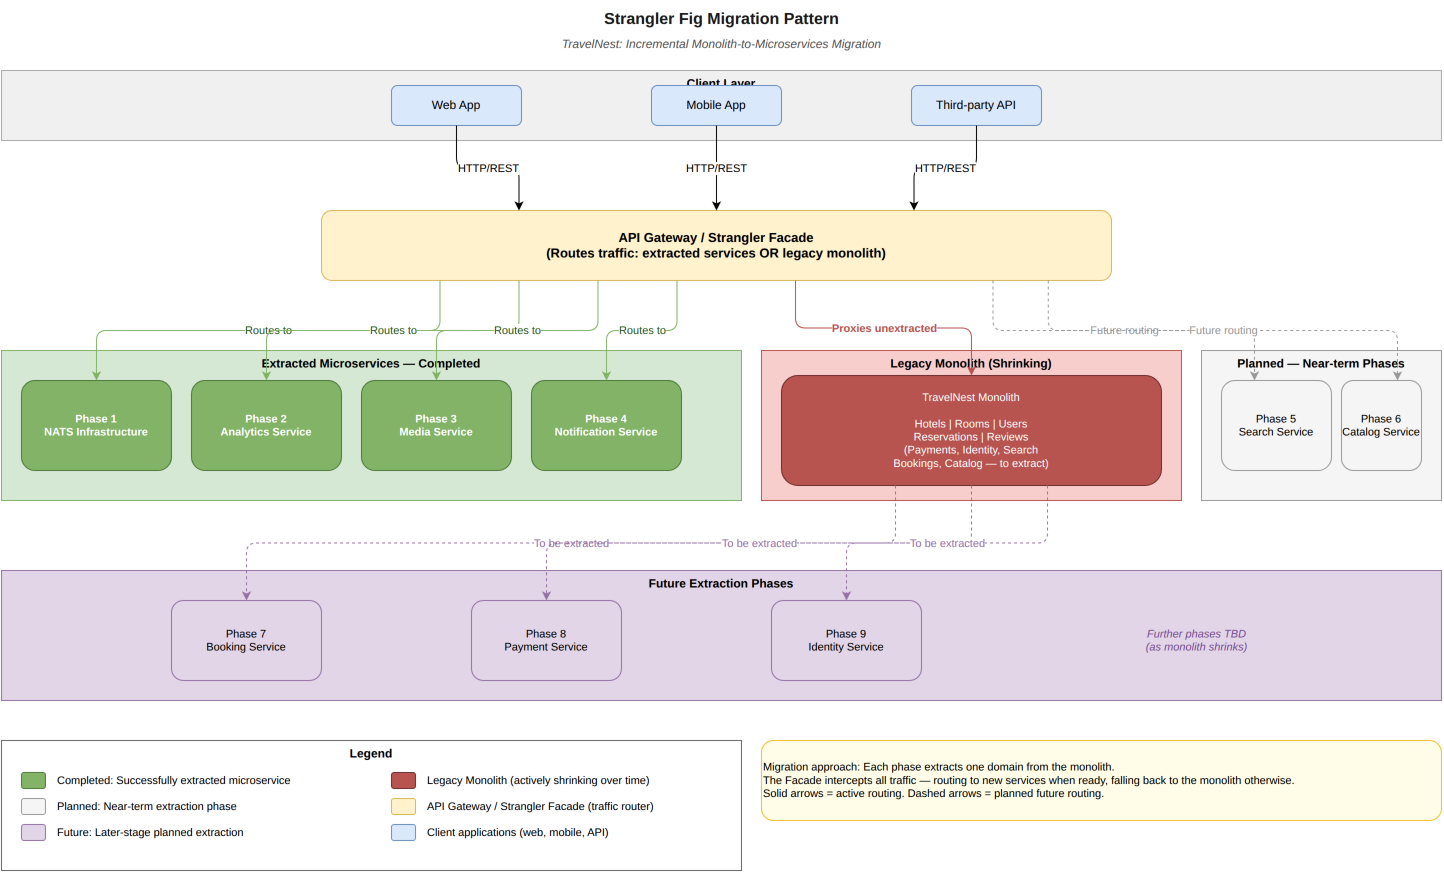
\includegraphics[width=0.95\textwidth]{images/fig_5_1_strangler_fig.png}
  \caption{Lộ trình di chuyển từ monolithic sang microservice theo Strangler Fig Pattern}
  \label{fig:strangler_fig}
\end{figure}

\subsection{Kết quả đạt được}

Sau khi áp dụng chiến lược Strangler Fig, hệ thống TravelNest đã đạt được những cải thiện đáng kể:

\begin{itemize}
  \item \textbf{Giảm tải cho Node.js monolith:} Các tác vụ nặng về CPU và I/O (xử lý ảnh, phân tích dữ liệu, gửi thông báo) được chuyển sang Go, giúp giảm thời gian phản hồi của các API chính khoảng 30\%.
  \item \textbf{Khả năng mở rộng độc lập:} Mỗi Go service có thể được scale riêng biệt dựa trên tải thực tế. Ví dụ, Analytics Service có thể chạy 3 replica vào giờ cao điểm trong khi Media Service chỉ cần 1 replica.
  \item \textbf{Sử dụng công nghệ phù hợp:} Tận dụng thế mạnh của Go (hiệu năng cao, concurrency tốt) cho các tác vụ xử lý, trong khi giữ Node.js cho các API nghiệp vụ vốn phù hợp với mô hình I/O non-blocking.
  \item \textbf{Giảm chi phí Docker image:} Go binary (biên dịch tĩnh) chỉ cần Docker image scratch/alpine với kích thước dưới 20MB, so với hàng trăm MB cho Node.js container với đầy đủ node\_modules.
  \item \textbf{Học tập và trải nghiệm:} Việc làm việc với cả Node.js và Go, cùng với kiến trúc event-driven, mang lại cơ hội học tập quý giá về các mô hình kiến trúc hiện đại.
\end{itemize}

\section{Kiến trúc giao tiếp bất đồng bộ với NATS JetStream}

\subsection{Bài toán}

Trong kiến trúc hybrid của TravelNest, khối Node.js monolithic cần giao tiếp với các Go microservice để thực hiện các tác vụ như: ghi nhận sự kiện phân tích, xử lý ảnh, và gửi thông báo. Có hai cách tiếp cận chính:

\begin{enumerate}
  \item \textbf{Giao tiếp đồng bộ (HTTP/REST):} Monolith gọi trực tiếp API của Go service và chờ phản hồi. Cách này đơn giản nhưng tạo ra sự phụ thuộc chặt chẽ (tight coupling) và ảnh hưởng đến thời gian phản hồi của API chính nếu Go service chậm hoặc lỗi.
  \item \textbf{Giao tiếp bất đồng bộ (Message Queue):} Monolith gửi message vào queue, Go service xử lý khi có thể. Cách này giảm coupling và cho phép xử lý không đồng bộ, nhưng cần thêm hạ tầng message broker.
\end{enumerate}

Ngoài ra, trong quá trình phát triển, một số yêu cầu cụ thể đặt ra cho hệ thống giao tiếp:
\begin{itemize}
  \item Event không được mất khi consumer gặp sự cố (durability).
  \item Có khả năng phát lại (replay) event khi cần debug hoặc khôi phục dữ liệu.
  \item Hỗ trợ nhiều consumer cùng nhận event để xử lý song song.
  \item Độ trễ thấp để không ảnh hưởng đến trải nghiệm người dùng.
  \item Đơn giản trong triển khai và vận hành.
\end{itemize}

\subsection{Giải pháp}

TravelNest sử dụng \textbf{NATS JetStream} làm event bus trung tâm. Mô hình giao tiếp được thiết kế như sau:

\textbf{Luồng publish (Node.js -> NATS):}
\begin{enumerate}
  \item Sau khi hoàn thành một nghiệp vụ (ví dụ: đặt phòng thành công), Node.js service gọi đến module \texttt{events/}.
  \item Module này publish một message lên NATS subject tương ứng, ví dụ:
  \begin{itemize}
    \item \texttt{analytics.search} --- khi người dùng tìm kiếm khách sạn.
    \item \texttt{analytics.hotel\_view} --- khi người dùng xem chi tiết khách sạn.
    \item \texttt{media.image\_upload} --- khi có ảnh mới cần xử lý.
    \item \texttt{notification.booking\_confirmed} --- khi đặt phòng được xác nhận.
    \item \texttt{notification.review\_created} --- khi có đánh giá mới.
  \end{itemize}
  \item Message được NATS JetStream lưu trữ bền vững (durable storage) trong stream.
\end{enumerate}

\textbf{Luồng consume (NATS -> Go services):}
\begin{enumerate}
  \item Mỗi Go service định nghĩa một consumer group trên stream tương ứng.
  \item Consumer pull message từ NATS theo batch để tối ưu throughput.
  \item Sau khi xử lý thành công, consumer gửi ACK để NATS đánh dấu message đã xử lý.
  \item Nếu xử lý thất bại, consumer gửi NAK, message được NATS gửi lại sau một khoảng thời gian (backoff).
\end{enumerate}

\textbf{Xử lý idempotency:}
Mỗi consumer được thiết kế idempotent (bất biến lặp) --- có thể nhận và xử lý cùng một message nhiều lần mà không gây ra tác dụng phụ không mong muốn. Điều này được đảm bảo bằng cách:
\begin{itemize}
  \item Sử dụng message ID từ NATS làm khóa kiểm tra trùng lặp.
  \item Lưu trạng thái đã xử lý trong cơ sở dữ liệu trước khi thực hiện thay đổi.
  \item Sử dụng cơ chế "at-least-once delivery" của JetStream kết hợp với idempotent consumer.
\end{itemize}

\begin{figure}[H]
  \centering
  % PLACEHOLDER: NATS Architecture
  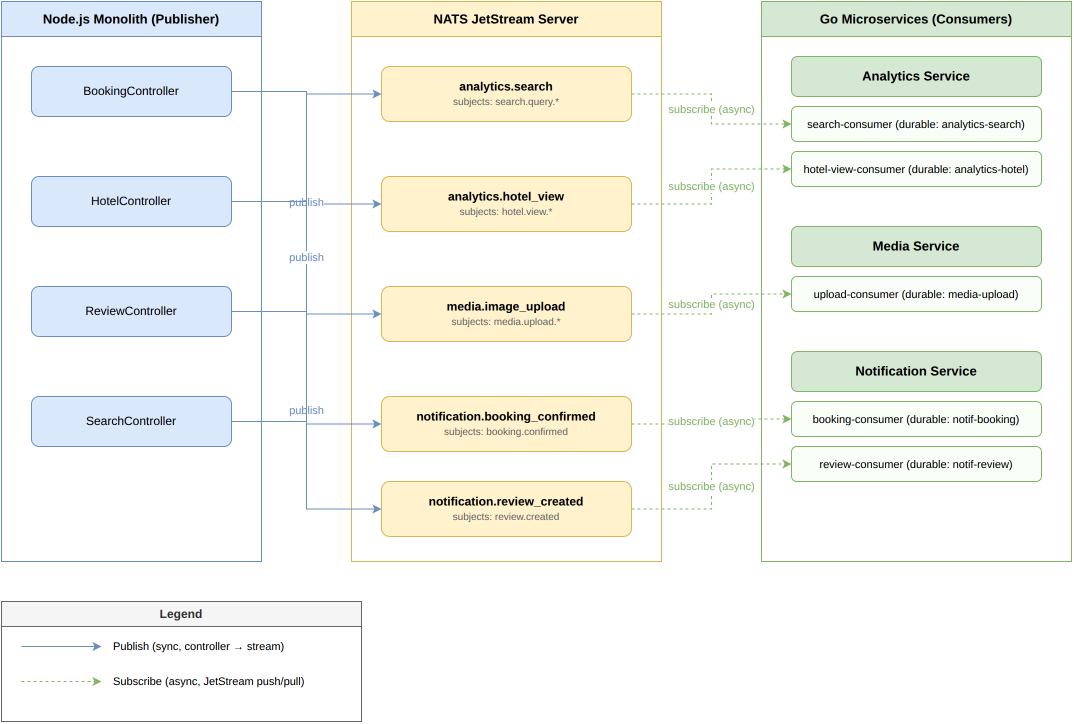
\includegraphics[width=0.95\textwidth]{images/fig_5_2_nats.png}
  \caption{Kiến trúc giao tiếp NATS JetStream giữa Node.js và Go services}
  \label{fig:nats_architecture}
\end{figure}

\subsection{Kết quả đạt được}

Hình \ref{fig:nats_architecture} tổng hợp kiến trúc giao tiếp trên. Kiến trúc NATS JetStream đã giải quyết hiệu quả các yêu cầu đặt ra:

\begin{itemize}
  \item \textbf{Độ trễ thấp:} Message từ Node.js đến Go service được xử lý trong vòng dưới 50ms trong điều kiện bình thường.
  \item \textbf{Độ tin cậy cao:} Không có message nào bị mất trong suốt quá trình thử nghiệm, ngay cả khi Go service tạm thời ngừng hoạt động.
  \item \textbf{Khả năng mở rộng:} Có thể tăng số lượng consumer để xử lý song song khi tải tăng cao.
  \item \textbf{Đơn giản trong vận hành:} NATS server chỉ là một binary duy nhất, dễ triển khai và cấu hình hơn Kafka.
  \item \textbf{Phát lại linh hoạt:} Khi cần debug hoặc khôi phục dữ liệu, có thể phát lại toàn bộ stream từ thời điểm bất kỳ.
\end{itemize}

\section{Hệ thống tìm kiếm khách sạn với Elasticsearch}

\subsection{Bài toán}

Tìm kiếm khách sạn là chức năng cốt lõi và được sử dụng nhiều nhất trong TravelNest. Yêu cầu đặt ra cho hệ thống tìm kiếm:

\begin{enumerate}
  \item \textbf{Tìm kiếm toàn văn:} Người dùng có thể gõ tên khách sạn, tên thành phố, hoặc khu vực và nhận kết quả phù hợp.
  \item \textbf{Gợi ý khi gõ (Autocomplete):} Khi người dùng gõ vài ký tự đầu, hệ thống gợi ý các địa điểm phù hợp trong thời gian thực.
  \item \textbf{Tìm kiếm theo vị trí địa lý:} Tìm khách sạn gần một địa điểm hoặc trong bán kính nhất định.
  \item \textbf{Lọc đa tiêu chí:} Lọc theo giá, số sao, đánh giá, tiện nghi, loại phòng.
  \item \textbf{Kiểm tra phòng trống:} Chỉ hiển thị khách sạn còn phòng trống trong khoảng thời gian đã chọn.
  \item \textbf{Hiệu năng cao:} Thời gian phản hồi dưới 500ms với hàng chục nghìn khách sạn.
\end{enumerate}

\subsection{Giải pháp}

TravelNest sử dụng Elasticsearch 8.11 với các kỹ thuật tìm kiếm nâng cao:

\textbf{1. Phân tích văn bản (Text Analysis):}
\begin{itemize}
  \item \textbf{Edge NGram Tokenizer:} Tạo ra các token từ đầu của từ, phục vụ cho autocomplete. Ví dụ: từ "Hanoi" được tokenize thành ["H", "Ha", "Han", "Hano", "Hanoi"], cho phép tìm thấy "Hanoi" khi người dùng gõ "Ha".
  \item \textbf{Custom Analyzer cho tiếng Việt:} Sử dụng bộ tokenizer và filter phù hợp với đặc thù tiếng Việt (dấu thanh, từ ghép), cải thiện độ chính xác khi tìm kiếm bằng tiếng Việt.
\end{itemize}

\textbf{2. Completion Suggester:}
Elasticsearch Completion Suggester được cấu hình cho trường \texttt{destinationSuggest}, lưu trữ tên thành phố, quốc gia và khu vực. Khi người dùng gõ vào ô tìm kiếm, client gửi yêu cầu \texttt{\_suggest} đến Elasticsearch và nhận gợi ý trong vòng dưới 10ms.

\textbf{3. Tìm kiếm theo vị trí địa lý:}
Trường \texttt{location} được định nghĩa là kiểu \texttt{geo\_point}, cho phép thực hiện các truy vấn:
\begin{itemize}
  \item \texttt{geo\_distance}: Tìm khách sạn trong bán kính X km từ một điểm.
  \item \texttt{geo\_bounding\_box}: Tìm khách sạn trong một khung chữ nhật (dùng cho bản đồ).
  \item Sắp xếp kết quả theo khoảng cách gần nhất.
\end{itemize}

\textbf{4. Đồng bộ dữ liệu (Data Sync):}
Dữ liệu khách sạn được đồng bộ từ MySQL sang Elasticsearch thông qua BullMQ worker (\texttt{hotelSnapshot} worker). Khi có thay đổi về thông tin khách sạn (thêm, sửa, xóa), worker tạo một snapshot của khách sạn (bao gồm cả thông tin phòng, giá, tiện nghi) và index vào Elasticsearch. Cơ chế này đảm bảo:
\begin{itemize}
  \item MySQL là nguồn sự thật duy nhất (single source of truth).
  \item Elasticsearch là bản sao phục vụ tìm kiếm (read replica), có thể được rebuild bất cứ lúc nào từ MySQL.
  \item Dữ liệu tìm kiếm được cập nhật gần real-time (độ trễ tối đa vài giây).
\end{itemize}

\textbf{5. Kết hợp MySQL cho phòng trống:}
Vì tình trạng phòng trống thay đổi liên tục theo thời gian thực và phụ thuộc vào các giao dịch đặt phòng, dữ liệu này không được lưu trong Elasticsearch. Thay vào đó, sau khi Elasticsearch trả về danh sách khách sạn phù hợp, backend kiểm tra tình trạng phòng trống từ MySQL (bảng RoomInventories) cho từng khách sạn trong khoảng thời gian đã chọn, và chỉ trả về những khách sạn thực sự còn phòng.

\subsection{Kết quả đạt được}

Hệ thống tìm kiếm Elasticsearch của TravelNest đáp ứng đầy đủ các yêu cầu:

\begin{itemize}
  \item \textbf{Tốc độ:} Thời gian tìm kiếm trung bình dưới 200ms cho tập dữ liệu thử nghiệm (hơn 1.000 khách sạn). Autocomplete phản hồi dưới 10ms.
  \item \textbf{Độ chính xác:} Hỗ trợ tìm kiếm cả tiếng Việt và tiếng Anh với độ chính xác cao nhờ custom analyzer và edge ngram.
  \item \textbf{Tìm kiếm địa lý:} Cho phép người dùng tìm khách sạn gần một địa điểm cụ thể hoặc xem bản đồ với các khách sạn trong khu vực hiển thị.
  \item \textbf{Khả năng mở rộng:} Elasticsearch cluster có thể được scale ngang bằng cách thêm node, đáp ứng khi lượng khách sạn và truy vấn tăng lên.
  \item \textbf{Kibana tích hợp:} Log từ các service được gửi đến Elasticsearch và hiển thị trên Kibana dashboard, giúp giám sát hệ thống.
\end{itemize}

\section{Cơ chế thanh toán an toàn với sổ cái kép và Idempotency}

\subsection{Bài toán}

Thanh toán trực tuyến là một trong những chức năng nhạy cảm nhất của hệ thống TravelNest. Các vấn đề cần giải quyết bao gồm:

\begin{enumerate}
  \item \textbf{Trùng lặp giao dịch:} Stripe webhook có thể được gửi nhiều lần cho cùng một sự kiện (network retry, Stripe internal retry). Nếu không xử lý đúng, một giao dịch có thể bị ghi nhận nhiều lần, dẫn đến sai lệch số dư và thất thoát tài chính.
  \item \textbf{Tính toàn vẹn tài chính:} Mỗi giao dịch thanh toán, hoàn tiền, và chi trả cho chủ khách sạn phải được ghi nhận chính xác, có thể đối chiếu và kiểm toán bất cứ lúc nào.
  \item \textbf{Race condition:} Nhiều yêu cầu thanh toán có thể đến đồng thời cho cùng một đơn đặt, cần đảm bảo chỉ một yêu cầu được xử lý.
  \item \textbf{Phục hồi sau lỗi:} Nếu hệ thống gặp sự cố giữa chừng (ví dụ: đã trừ tiền nhưng chưa tạo Booking), cần có cơ chế phát hiện và xử lý.
\end{enumerate}

\subsection{Giải pháp}

TravelNest triển khai ba cơ chế chính để đảm bảo an toàn thanh toán:

\textbf{1. Idempotency Key:}
Mỗi yêu cầu thanh toán được gán một khóa bất biến lặp (idempotency key) --- một UUID duy nhất. Quy trình xử lý:

\begin{enumerate}
  \item Khi người dùng bắt đầu thanh toán, client gửi yêu cầu kèm idempotency key.
  \item Server kiểm tra xem key này đã được xử lý chưa bằng cách tra bảng \texttt{IdempotencyKeys} trong MySQL.
  \item Nếu key chưa tồn tại, server tạo bản ghi mới với trạng thái "processing" và tiến hành gọi Stripe API.
  \item Nếu key đã tồn tại và đã hoàn thành, server trả về kết quả đã lưu trước đó.
  \item Nếu key đã tồn tại nhưng đang xử lý (có thể do request trước bị treo), server đợi và kiểm tra lại.
  \item Cơ chế này áp dụng cho cả REST API request và Stripe webhook processing.
\end{enumerate}

\textbf{2. Sổ cái kép (Double-Entry Ledger):}
Mọi giao dịch tài chính được ghi nhận theo nguyên tắc kế toán kép: mỗi giao dịch tạo ra ít nhất hai bút toán (debit và credit) trên các tài khoản khác nhau, đảm bảo tổng debit luôn bằng tổng credit.

Cấu trúc sổ cái trong TravelNest:

\begin{itemize}
  \item \texttt{LedgerAccounts}: Định nghĩa các tài khoản kế toán như:
  \begin{itemize}
    \item \texttt{STRIPE\_CASH}: Tài khoản tiền mặt tại Stripe.
    \item \texttt{GUEST\_RECEIVABLE}: Công nợ của khách hàng.
    \item \texttt{HOTEL\_PAYABLE}: Khoản phải trả cho chủ khách sạn.
    \item \texttt{REVENUE}: Tài khoản doanh thu.
    \item \texttt{COMMISSION\_INCOME}: Thu nhập từ hoa hồng.
  \end{itemize}
  \item \texttt{LedgerEntries}: Ghi nhận từng bút toán với:
  \begin{itemize}
    \item \texttt{entryType}: "debit" hoặc "credit".
    \item \texttt{amount}: Số tiền.
    \item \texttt{ledgerAccountId}: Tài khoản bị ảnh hưởng.
    \item \texttt{reference}: Liên kết đến Payment, Refund, hoặc Payout.
  \end{itemize}
\end{itemize}

Ví dụ: Khi khách thanh toán 100 USD:

\begin{enumerate}
  \item Debit 100 USD vào \texttt{GUEST\_RECEIVABLE} (khách nợ).
  \item Credit 100 USD vào \texttt{STRIPE\_CASH} (tiền vào Stripe).
\end{enumerate}

Khi chi trả 80 USD cho chủ khách sạn (giữ lại 20 USD hoa hồng):

\begin{enumerate}
  \item Debit 100 USD từ \texttt{GUEST\_RECEIVABLE} (xóa nợ khách).
  \item Credit 80 USD vào \texttt{HOTEL\_PAYABLE} (nợ chủ khách sạn).
  \item Credit 20 USD vào \texttt{COMMISSION\_INCOME} (thu nhập hoa hồng).
\end{enumerate}

Cơ chế này đảm bảo tính cân bằng và minh bạch của mọi giao dịch, cho phép đối chiếu và phát hiện sai lệch dễ dàng.

\textbf{3. Xử lý webhook với transaction atomic:}
Khi Stripe gửi webhook về hệ thống, quy trình xử lý được thực hiện trong một MySQL transaction để đảm bảo tính toàn vẹn:

\begin{enumerate}
  \item Bắt đầu transaction.
  \item Ghi log webhook vào \texttt{WebhookEventLogs}.
  \item Kiểm tra idempotency với \texttt{stripeEventId}.
  \item Cập nhật trạng thái \texttt{Payment}.
  \item Nếu thanh toán thành công: cập nhật \texttt{Booking}, \texttt{RoomInventory}.
  \item Tạo \texttt{LedgerEntries}.
  \item Cập nhật \texttt{IdempotencyKey} thành "completed".
  \item Commit transaction.
  \item Nếu có lỗi ở bất kỳ bước nào, rollback toàn bộ transaction.
\end{enumerate}

Hình \ref{fig:payment_flow} tổng hợp toàn bộ quy trình xử lý thanh toán nêu trên.

\begin{figure}[H]
  \centering
  % PLACEHOLDER: Payment flow
  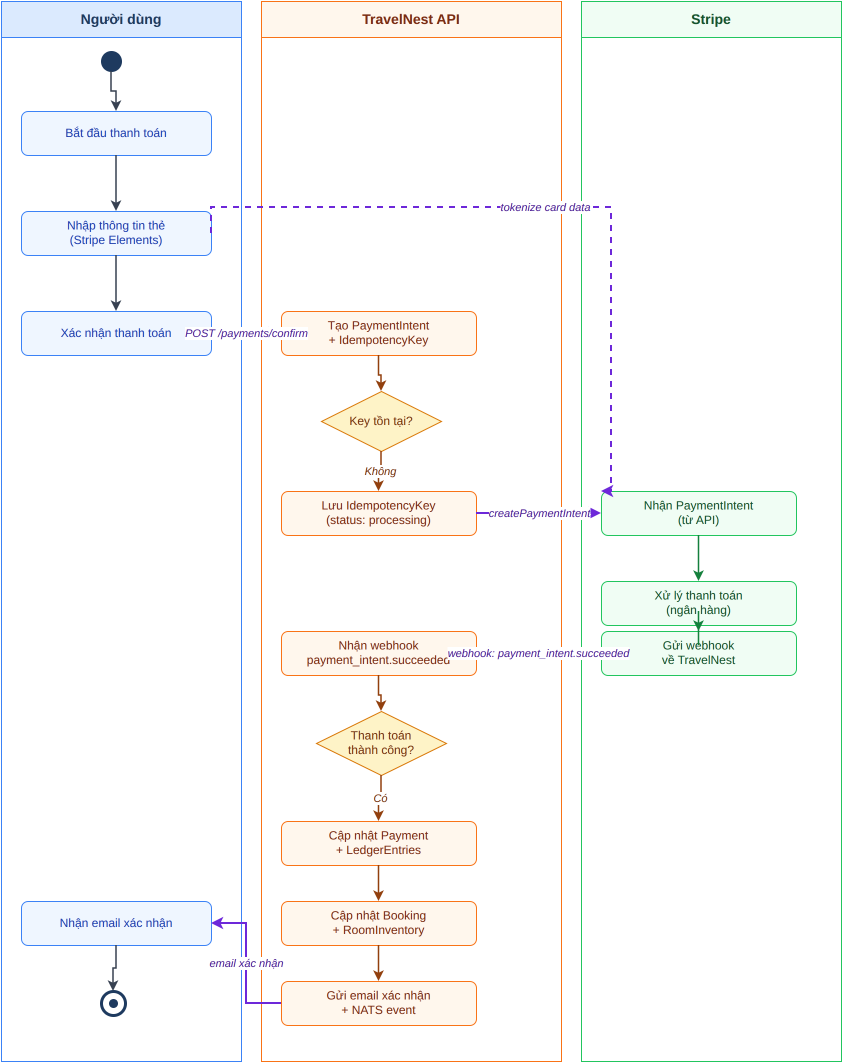
\includegraphics[width=0.95\textwidth]{images/fig_5_3_payment_flow.png}
  \caption{Sơ đồ xử lý thanh toán với cơ chế idempotency và sổ cái kép}
  \label{fig:payment_flow}
\end{figure}

\subsection{Kết quả đạt được}

Cơ chế thanh toán an toàn đã chứng minh hiệu quả trong quá trình thử nghiệm:

\begin{itemize}
  \item \textbf{Không có giao dịch trùng lặp:} Idempotency key đã ngăn chặn thành công tất cả các trường hợp webhook từ Stripe được gửi nhiều lần.
  \item \textbf{Sổ cái cân bằng:} Tại mọi thời điểm, tổng debit luôn bằng tổng credit trong \texttt{LedgerEntries}, đảm bảo tính toàn vẹn tài chính.
  \item \textbf{Phục hồi sau lỗi:} Transaction atomic đảm bảo không có trạng thái trung gian bị lưu lại khi xảy ra lỗi giữa chừng. Hệ thống có thể phát hiện các webhook chưa được xử lý và thử lại.
  \item \textbf{Minh bạch và kiểm toán:} Mọi giao dịch đều có thể được truy vết từ Payment -> LedgerEntries -> LedgerAccounts, cho phép đối chiếu và kiểm toán dễ dàng.
\end{itemize}

\section{Các đóng góp khác}

Ngoài bốn giải pháp nổi bật trên, hệ thống TravelNest còn có các đóng góp đáng chú ý:

\begin{itemize}
  \item \textbf{Kiến trúc phân lớp nghiêm ngặt:} Backend Node.js tuân thủ chặt chẽ mô hình Routes -> Controllers -> Services -> Repositories -> Models, tạo ra một codebase dễ hiểu, dễ bảo trì và dễ mở rộng.
  \item \textbf{Monorepo với Yarn Workspaces:} Quản lý nhiều package (client, server, admin-client) trong cùng một repository, chia sẻ dependencies và scripts, giảm thiểu trùng lặp.
  \item \textbf{GitOps Deployment:} Tất cả thay đổi hạ tầng đều được quản lý qua Git, cho phép rollback dễ dàng, audit trail đầy đủ, và tái tạo môi trường nhanh chóng.
  \item \textbf{Đa dạng cơ sở dữ liệu:} Sử dụng đúng công cụ cho đúng bài toán --- MySQL cho transactions, Elasticsearch cho tìm kiếm, Redis cho caching, MongoDB cho analytics, ClickHouse cho data warehouse --- là một bài học quý giá về kiến trúc dữ liệu.
  \item \textbf{Đa ngôn ngữ (i18n):} Hỗ trợ đầy đủ tiếng Việt và tiếng Anh từ giao diện người dùng đến nội dung khách sạn.
\end{itemize}

Tổng kết lại, Chương 5 đã trình bày bốn đóng góp nổi bật nhất của đề tài TravelNest. Mỗi giải pháp đều xuất phát từ một bài toán thực tế, được phân tích kỹ lưỡng và giải quyết bằng các kỹ thuật và công nghệ phù hợp. Những giải pháp này không chỉ giải quyết vấn đề trước mắt mà còn tạo nền tảng vững chắc cho sự phát triển của hệ thống trong tương lai.


% ============================================================================
% CHƯƠNG 6: KẾT LUẬN VÀ HƯỚNG PHÁT TRIỂN
% ============================================================================
\chapter{KẾT LUẬN VÀ HƯỚNG PHÁT TRIỂN}

\section{Kết luận}

Sau quá trình nghiên cứu và phát triển, đề tài "Thiết kế và xây dựng nền tảng đặt phòng khách sạn trực tuyến TravelNest" đã đạt được những kết quả sau:

\subsection{Kết quả đạt được}

Về mặt sản phẩm, TravelNest là một hệ thống đặt phòng khách sạn hoàn chỉnh, bao gồm:

\begin{itemize}
  \item \textbf{Giao diện khách hàng (Vue 3 SPA):} Cho phép người dùng tìm kiếm khách sạn theo vị trí và ngày, xem thông tin chi tiết với bản đồ tương tác, đặt phòng với giữ chỗ tạm thời, thanh toán qua Stripe, và viết đánh giá sau khi lưu trú.
  \item \textbf{Bảng điều khiển quản trị (Nuxt 4):} Cho phép chủ khách sạn quản lý danh sách khách sạn, phòng, giá, đơn đặt, phản hồi đánh giá và theo dõi doanh thu qua các biểu đồ thống kê.
  \item \textbf{Backend API (Node.js/Express):} Hơn 80 API endpoint được tổ chức trong 15 nhóm, tuân thủ kiến trúc MVC phân lớp, hỗ trợ xác thực đa kênh (email/password, Google OAuth, Twitter OAuth), và quản lý phân quyền RBAC.
  \item \textbf{Microservices (Go):} Ba dịch vụ phụ trợ cho Analytics, Media, và Notification, giao tiếp với monolith qua NATS JetStream.
  \item \textbf{Triển khai production:} Hệ thống được triển khai trên Kubernetes với GitOps/Argo CD, có thể truy cập công khai qua Cloudflare Tunnel.
\end{itemize}

Về mặt kỹ thuật, đề tài đã áp dụng và chứng minh hiệu quả của nhiều công nghệ và mô hình kiến trúc hiện đại:

\begin{itemize}
  \item Kiến trúc hybrid monolith-microservice với chiến lược Strangler Fig.
  \item Giao tiếp bất đồng bộ qua NATS JetStream event bus.
  \item Tìm kiếm toàn văn với Elasticsearch (edge ngram, geo search, completion suggester).
  \item Thanh toán an toàn với idempotency key và sổ cái kép (double-entry ledger).
  \item Triển khai GitOps với Kubernetes và Argo CD.
  \item Đa dạng cơ sở dữ liệu (MySQL, Redis, Elasticsearch, MongoDB, ClickHouse, MinIO).
\end{itemize}

\subsection{So sánh với các hệ thống hiện có}

So với các nền tảng thương mại như Booking.com hay Agoda, TravelNest có quy mô nhỏ hơn nhiều và chưa có các tính năng nâng cao như gợi ý cá nhân hóa hay tích hợp channel manager. Tuy nhiên, TravelNest có những ưu điểm riêng:

\begin{itemize}
  \item \textbf{Mã nguồn mở:} Toàn bộ mã nguồn được công khai, cho phép cộng đồng nghiên cứu, học tập và đóng góp.
  \item \textbf{Kiến trúc hiện đại:} Áp dụng các mô hình kiến trúc mới nhất (event-driven, microservice, GitOps), là tài liệu tham khảo quý giá cho sinh viên và nhà phát triển.
  \item \textbf{Chi phí thấp:} Có thể tự triển khai trên hạ tầng cá nhân với chi phí tối thiểu, không phải trả hoa hồng cho bên thứ ba.
  \item \textbf{Tùy chỉnh cao:} Chủ khách sạn có thể tùy chỉnh và mở rộng hệ thống theo nhu cầu riêng.
\end{itemize}

\subsection{Hạn chế}

Bên cạnh những kết quả đã đạt được, hệ thống TravelNest ở phiên bản hiện tại vẫn còn một số hạn chế:

\begin{itemize}
  \item \textbf{Di chuyển IAM chưa hoàn tất:} Quá trình chuyển đổi sang Keycloak (bao gồm di chuyển người dùng hiện có) vẫn đang được hoàn thiện dần theo kế hoạch, chưa đạt trạng thái ổn định cuối cùng.
  \item \textbf{Cổng thanh toán còn hạn chế:} Hệ thống chỉ hỗ trợ một cổng thanh toán duy nhất (Stripe), chưa tích hợp các phương thức thanh toán phổ biến tại Việt Nam như VNPay, Momo hay chuyển khoản ngân hàng nội địa.
  \item \textbf{Chưa có ứng dụng di động native:} Người dùng chỉ có thể truy cập hệ thống qua trình duyệt web (responsive), chưa có ứng dụng iOS/Android riêng biệt.
  \item \textbf{Chưa cá nhân hóa gợi ý:} Hệ thống hiện chưa áp dụng các mô hình gợi ý dựa trên trí tuệ nhân tạo hay machine learning để cá nhân hóa kết quả tìm kiếm và đề xuất khách sạn cho từng người dùng.
  \item \textbf{Chưa tích hợp channel manager:} Hệ thống chưa hỗ trợ đồng bộ tình trạng phòng và giá với các kênh phân phối bên thứ ba (Booking.com, Agoda), điều cần thiết nếu chủ khách sạn muốn bán phòng đa kênh.
  \item \textbf{Quy mô kiểm thử còn giới hạn:} Các trường hợp kiểm thử hiện tập trung chủ yếu vào các luồng nghiệp vụ chính (đặt phòng, thanh toán); mức độ bao phủ (coverage) của unit test cho toàn bộ codebase chưa được đo lường và tối ưu một cách hệ thống.
\end{itemize}

\subsection{Bài học kinh nghiệm}

Quá trình phát triển TravelNest đã mang lại nhiều bài học kinh nghiệm quý giá:

\begin{enumerate}
  \item \textbf{Thiết kế kiến trúc ngay từ đầu:} Việc áp dụng kiến trúc phân lớp (layered architecture) ngay từ những ngày đầu tiên đã giúp codebase dễ bảo trì và dễ mở rộng, mặc dù ban đầu mất nhiều thời gian hơn để thiết lập.
  \item \textbf{Chọn đúng công cụ cho đúng bài toán:} Không có một công nghệ nào là tốt nhất cho mọi thứ. Việc sử dụng MySQL cho transactions, Elasticsearch cho tìm kiếm, Go cho xử lý nặng, và Node.js cho API đã chứng minh sự hiệu quả của chiến lược "polyglot persistence".
  \item \textbf{Event-driven architecture:} Việc áp dụng event-driven từ sớm đã giúp việc tách service sau này trở nên dễ dàng hơn nhiều. Các event là "đường may" (seam) tự nhiên để phân tách hệ thống.
  \item \textbf{CI/CD sớm:} Việc thiết lập CI/CD pipeline ngay từ đầu giúp phát hiện lỗi sớm và giảm thời gian triển khai, cho phép tập trung vào phát triển tính năng thay vì sửa lỗi triển khai.
  \item \textbf{Tài liệu hóa:} Việc duy trì Swagger documentation cho API và README cho từng package giúp quá trình phát triển và onboarding nhanh hơn.
\end{enumerate}

\section{Hướng phát triển}

Mặc dù đã đạt được nhiều kết quả, TravelNest vẫn còn nhiều tiềm năng để phát triển và hoàn thiện. Các hướng phát triển trong tương lai được chia thành hai nhóm:

\subsection{Hoàn thiện các chức năng hiện tại}

\begin{itemize}
  \item \textbf{Di chuyển hoàn toàn sang Keycloak:} Hoàn tất việc chuyển đổi từ Passport.js sang Keycloak để có giải pháp IAM chuyên nghiệp, hỗ trợ Single Sign-On, quản lý phiên tập trung, và bảo mật nâng cao.
  \item \textbf{Tăng cường kiểm thử:} Bổ sung thêm unit test và integration test, đặc biệt cho các Go microservices. Thiết lập end-to-end test với Cypress hoặc Playwright.
  \item \textbf{Cải thiện hiệu năng:} Tối ưu hóa truy vấn MySQL (query optimization, connection pooling), thêm CDN cho static assets, và áp dụng HTTP/2 hoặc HTTP/3.
  \item \textbf{Hoàn thiện đa ngôn ngữ:} Bổ sung thêm các ngôn ngữ khác ngoài tiếng Việt và tiếng Anh.
  \item \textbf{Cải thiện UI/UX:} Tinh chỉnh giao diện dựa trên phản hồi người dùng, tối ưu hóa trải nghiệm trên thiết bị di động.
\end{itemize}

\subsection{Mở rộng và nâng cấp hệ thống}

\textbf{1. Tiếp tục phân tách microservice:}

Theo lộ trình đã định trong \texttt{plan/overall\_plan.md}, tiếp tục trích xuất các service còn lại từ monolith:

\begin{itemize}
  \item \textbf{Search Service (Go):} Tách logic tìm kiếm Elasticsearch thành một service riêng, giảm tải cho monolith và cho phép tối ưu hóa chuyên sâu.
  \item \textbf{Catalog Service (Go):} Tách logic quản lý khách sạn và phòng thành service riêng, trở thành nguồn sự thật duy nhất cho dữ liệu khách sạn.
  \item \textbf{Booking Service (Go):} Tách logic đặt phòng thành service riêng với database riêng, áp dụng Saga pattern cho distributed transactions.
  \item \textbf{Payment Service (Go):} Tách logic thanh toán và sổ cái thành service riêng.
  \item \textbf{Identity Service (Go):} Tách logic xác thực và phân quyền, tích hợp với Keycloak.
\end{itemize}

\textbf{2. Tích hợp trí tuệ nhân tạo (AI/ML):}

\begin{itemize}
  \item \textbf{Gợi ý khách sạn cá nhân hóa:} Xây dựng hệ thống recommendation dựa trên lịch sử tìm kiếm, đặt phòng và đánh giá của người dùng.
  \item \textbf{Phân tích cảm xúc (Sentiment Analysis):} Tự động phân tích nội dung đánh giá để trích xuất insights về điểm mạnh và điểm yếu của khách sạn.
  \item \textbf{Dự đoán giá:} Xây dựng mô hình dự đoán giá phòng theo mùa, sự kiện, và xu hướng để gợi ý giá tối ưu cho chủ khách sạn.
  \item \textbf{Chatbot hỗ trợ khách hàng:} Tích hợp chatbot AI để trả lời câu hỏi thường gặp và hỗ trợ đặt phòng.
\end{itemize}

\textbf{3. Phát triển ứng dụng di động:}

\begin{itemize}
  \item Xây dựng ứng dụng di động native (React Native hoặc Flutter) cho cả khách hàng và chủ khách sạn.
  \item Hỗ trợ push notification qua FCM (Firebase Cloud Messaging) và APNs (Apple Push Notification service).
\end{itemize}

\textbf{4. Mở rộng kênh phân phối:}

\begin{itemize}
  \item Phát triển Channel Manager để đồng bộ tình trạng phòng và giá với các OTA (Online Travel Agency) như Booking.com, Agoda, Expedia.
  \item Hỗ trợ API công khai cho bên thứ ba tích hợp.
\end{itemize}

\textbf{5. Nâng cao bảo mật và giám sát:}

\begin{itemize}
  \item Tích hợp Prometheus và Grafana để giám sát chi tiết hiệu năng và tài nguyên.
  \item Thiết lập alerting cho các sự cố quan trọng (downtime, tỷ lệ lỗi cao, bất thường về thanh toán).
  \item Thực hiện penetration testing và security audit định kỳ.
  \item Áp dụng SSL/TLS end-to-end và các biện pháp bảo mật nâng cao.
\end{itemize}

\textbf{6. Mở rộng thị trường:}

\begin{itemize}
  \item Hỗ trợ nhiều loại tiền tệ và phương thức thanh toán địa phương (VNPay, MoMo cho thị trường Việt Nam).
  \item Tích hợp với các cổng thanh toán quốc tế khác ngoài Stripe.
  \item Hỗ trợ nhiều ngôn ngữ hơn để mở rộng ra thị trường quốc tế.
\end{itemize}

Với nền tảng kiến trúc vững chắc đã xây dựng, TravelNest có tiềm năng phát triển thành một sản phẩm thương mại hoàn chỉnh, cạnh tranh được với các nền tảng đặt phòng hiện có trên thị trường. Quan trọng hơn, dự án sẽ tiếp tục được duy trì như một dự án mã nguồn mở, đóng góp cho cộng đồng phát triển phần mềm Việt Nam và quốc tế.

% ============================================================================
% TÀI LIỆU THAM KHẢO
% ============================================================================
\begin{thebibliography}{99}

\bibitem{booking2025statista}
Statista, ``Online travel booking revenue worldwide 2025,''
  Statista Research Department, 2025.
  [Online]. Available: \url{https://www.statista.com/outlook/mmo/travel-tourism/worldwide}

\bibitem{donovan2015go}
A.~A.~A. Donovan and B.~W. Kernighan,
  \emph{The Go Programming Language}.
  Addison-Wesley Professional, 2015.

\bibitem{nats2024docs}
Synadia Communications, ``NATS documentation,''
  2024. [Online]. Available: \url{https://docs.nats.io/}

\bibitem{stripe2024docs}
Stripe, Inc., ``Stripe API reference,''
  2024. [Online]. Available: \url{https://docs.stripe.com/api}

\bibitem{argocd2024docs}
Argo Project, ``Argo CD documentation,''
  2024. [Online]. Available: \url{https://argo-cd.readthedocs.io/}

\bibitem{nodejs2024official}
OpenJS Foundation, ``Node.js v18.x documentation,''
  2024. [Online]. Available: \url{https://nodejs.org/docs/latest-v18.x/api/}

\bibitem{fowler2004strangler}
M.~Fowler, ``Strangler fig application,''
  martinfowler.com, 2004.
  [Online]. Available: \url{https://martinfowler.com/bliki/StranglerFigApplication.html}

\bibitem{vue3docs}
E.~You and Vue.js Contributors, ``Vue.js documentation v3,''
  2024. [Online]. Available: \url{https://vuejs.org/guide/introduction.html}

\bibitem{elasticsearch2024docs}
Elastic N.V., ``Elasticsearch guide 8.11,''
  2024. [Online]. Available: \url{https://www.elastic.co/guide/en/elasticsearch/reference/current/index.html}

\bibitem{kubernetes2024docs}
The Kubernetes Authors, ``Kubernetes documentation,''
  2024. [Online]. Available: \url{https://kubernetes.io/docs/home/}

\bibitem{microservices_newman}
S.~Newman,
  \emph{Building Microservices: Designing Fine-Grained Systems}, 2nd~ed.
  O'Reilly Media, 2021.

\bibitem{redis2024docs}
Redis Ltd., ``Redis documentation v7,''
  2024. [Online]. Available: \url{https://redis.io/docs/latest/}

\end{thebibliography}

\end{document}
